	%\documentclass[a4paper]{article}
	%\usepackage[a4paper, left=2cm, right=2cm, top=2cm, bottom=2cm]{geometry} % Este pacote altera a margem do documento
  
	\documentclass[a4paper,12pt]{book}
	%\usepackage[inner=2cm,outer=2cm,bindingoffset=2cm]{geometry}
    \usepackage[inner=2.5cm,outer=2cm,top=2cm,bottom=2cm,
    bindingoffset=5mm]{geometry}
	\usepackage[utf8]{inputenc} % Este pacote serve para acentuação
	\usepackage[brazil]{babel} % Este pacote coloca os nomes em pt-br
	\usepackage{indentfirst} % Este pacote aplica indentação
	\usepackage[svgnames, usenames, dvipsnames]{xcolor} % Modifica as cores
	\usepackage{amsmath}
	\usepackage{color}
	\usepackage{soul} % usei para realce em amarelo
	\usepackage{amsfonts}
	\usepackage{mathtools}
	\usepackage{tasks}
	\usepackage{multicol}
	\usepackage{multirow}
	\usepackage{graphicx} % Este pacote permite adicionar figuras
	\usepackage{float} % Força o posicionamento da figura
	%\usepackage{subcaption}   
	\usepackage{indentfirst}
	\usepackage{booktabs}
	\usepackage{hyperref}
\hypersetup{colorlinks,citecolor=black,filecolor=black,linkcolor=black,urlcolor=black} %
         
	\usepackage{fancyhdr}% estrutura o cabeçalho, rodapé, capa
	\usepackage{booktabs,multirow,bigstrut} % unir tabela gerada no excel
	\usepackage[T1]{fontenc}
	\usepackage{colortbl}
	\usepackage{booktabs}
	\usepackage{scalefnt}
    \usepackage{fontawesome5}%para fazer o simbolo do youtube
    \usepackage{yhmath}
	\usepackage{makecell}
    \usepackage{caption}
    \usepackage{bm}
    \usepackage{setspace}
    \usepackage{siunitx}
    \usepackage{amssymb}
    \usepackage{gensymb}
    \usepackage{tabularx}
    \usepackage{extarrows}
    \usepackage{booktabs}
    \usepackage{changepage} %function adjustwidth
    \usepackage{courier}
    \usepackage{scalefnt}
    \usepackage{epstopdf}
    \usepackage{gensymb}%para escrever 30° com \degree
	\usepackage{array}
	\usepackage{stackengine}[2013-09-11]% zero cortado
	   \newcommand\slashzero{\stackinset{c}{}{c}{}{/}{0}}
	\usepackage{icomma} %no space after commma
	\usepackage[skip=10pt plus1pt, indent=30pt]{parskip}
    \usepackage{lmodern}
    \usepackage[svgnames]{xcolor}
    \usepackage[most]{tcolorbox}%fundo dos exemplos coloridos
    \usetikzlibrary{shadows}%fundo dos exemplos coloridos
    \newcounter{exa}
        \tcbset{
        myexample/.style={
        enhanced,
        colback=white,
        colframe=minha_cor,
        fonttitle=\scshape,
        title={\refstepcounter{exa}exemplo~\theexa},
        title style={fill=minha_cor},
        coltitle=black,
        every box/.style={highlight math style={colback=minha_cor,colframe=minha_cor}}
        }}
        \newtcolorbox{texample}{myexample}
        %cor anterior = LightBlue!50!white
	   \definecolor{minha_cor}{HTML}{e5fcba}
        %cor anterior = E5FAEC
	\usepackage{tikz}     
	   \tikzset{every picture/.style={line width=0.75pt}} %set default line width to 0.75pt  
    \usepackage{pgfplots}
    \pgfplotsset{width=7cm,compat=1.18}

    \usetikzlibrary{intersections}
	\usepackage{multicol}
	   \setlength{\columnsep}{2cm}
	\usepackage[Bjornstrup]{fncychap}
	    \newcommand{\df}{\displaystyle\frac}
	
	   \newtcolorbox{mytextbox}[1][]{%
	   	sharp corners,
	   	enhanced,
	   	colback=white,
	   	height=10cm,
	   	attach title to upper,
	   	#1
	}

        % Código para funções trigonométricas

        \DeclareMathOperator{\sen}{sen}
        \DeclareMathOperator{\tg}{tg}
        \DeclareMathOperator{\cotg}{cotg}
        \DeclareMathOperator{\cossec}{cossec}
        \DeclareMathOperator{\arcsen}{arcsen}
        \DeclareMathOperator{\arctg}{arctg}

        %----------------------------

        
        % Define cores para a ilustração de frações
        
        \definecolor{fraccolor}{rgb}{0.72, 0.83, 0.51}
        
        %----------------------------
        
        
	
	%%%%%%%%%%%%%%% início do documento %%%%%%%%%%%%%%%
	\begin{document}
		\newgeometry{left=2cm,bottom=2cm}% retira a margem intercalada de livro
        
        \thispagestyle{empty}
		\vspace{2cm}
\begin{center}
	\bfseries \LARGE Universidade de São Paulo\\
	\vspace{1cm}
	\bfseries \Large Escola Superior de Agricultura ``Luiz de Queiroz''\\
	\vspace{1cm}
	\bfseries \Large Departamento de Ciências Exatas\\
	\vspace{5cm}
	\bfseries {\fontsize{32}{32}\selectfont Curso Pré-Cálculo}\\[0.5cm]
	\bfseries  \huge{\textbf{6$^a$ Edição}}\\
	\vspace{3cm}
	\normalsize{Última atualização em 24/02/2023}\\
	\vspace{5.5cm}
	\begin{minipage}[t]{.45\textwidth}
	    \raggedleft
        
\includegraphics[width=0.3\linewidth]{Figuras/brasao_esalq1.jpg}\hspace{0.5cm}
    \end{minipage}
    \begin{minipage}[t]{.45\textwidth}
        \raggedright
        \hspace{0.5cm}
\includegraphics[width=0.35\linewidth]{Figuras/usp_logo.jpg}
    \end{minipage}
\end{center}
		\newpage
  
		\restoregeometry  % volta a gerar margem intercalada como um livro	
		\thispagestyle{empty} %para não aparecer o número na 1°pag em branco
        
        \pagenumbering{roman}
        \cleardoublepage
        \setcounter{page}{0}
		\tableofcontents % índice
		%\thispagestyle{empty} %para não aparecer o número zero no índice.
		
		%\setcounter{page}{0} %para começar a contagem das páginas
        %----------------------------
		\pagestyle{fancy} % define o cabeçalho e rodapé das páginas
        %\thispagestyle{empty}
		\fancyhead[R]{
\includegraphics[width=0.08 \textwidth]{Figuras/usp_logo.jpg}}
		\fancyhead[C]{}
		\fancyhead[L]{
\includegraphics[width=0.15\textwidth]{Figuras/esalq.png}}
		\fancyfoot[L]{}
		\fancyfoot[C]{\thepage}
		\fancyfoot[R]{}
		\renewcommand{\headrulewidth}{0.4pt}
		\renewcommand{\footrulewidth}{0.4pt}  
        %----------------------------
        
        
        
		%\chapter{Introdução}

		%	Colocar a introdução\\
		
	\textbf{Pra lembrar a ordem dos módulos:}\\
	1.Operações básicas de frações\\
	2.Potenciação e radiciação\\
	3.Produtos Notáveis e Fatoração\\
	4.Logaritmo e Exponencial\\
	5.Equações e Inequações de 1º grau\\
	6.Equações e Inequações de 2º grau\\
	7.Equações modulares\\
	8.Trigonometria\\
	
	\textbf{As ordem dos conteúdos são !?}\\
	1-definição\\
	2-tipos de ocorrências em exemplos com exercícios resolvidos\\
	3-exercícios propostos\\
	4-respostas dos exercícios propostos\\



 
		
		\chapter{Operações básicas com frações}

		\pagenumbering{arabic} % And moving back to arabic numbering (1,2,3,4) for the body.
        \patchcmd{\chapter}
        {\clearpage}
        {\cleardoublepage}
        {}
        {}
  
		    \section{Fração}

    \noindent
	\textbf{Definição:} Uma FRAÇÃO é um número racional que representa uma ou mais partes de um todo, ou seja, é a forma de dividir alguma coisa por meio da razão de dois números, em que o \textbf{dividendo }é chamado de numerador (indica quantas partes do todo foram tomadas) e o \textbf{divisor} é conhecido como denominador (indica o total de partes iguais que o inteiro fora dividido).
        \begin{tcolorbox}[colback=white,colframe=minha_cor,coltitle=black,title=Definição] 
            \[
            \df{a}{b}
            \]
            \end{tcolorbox}	
            \hspace{-1.2cm} em que: ``$a$'' é o dividendo (numerador) e ``$b$'' é o divisor (denominador).
            
    Ao dividir uma pizza, por exemplo, a pizza é fracionada. Cada fatia representa uma parte da pizza, ou seja, uma FRAÇÃO. Geralmente ela é dividida em 8 pedaços, então cada pedaço de uma pizza representa $\frac{1}{8}$ (um oitavo) dela.
	
	\section{Tipos de Frações}
	
	\subsection{Frações Próprias}
	As frações são ditas próprias quando o valor numérico do numerador é menor que o valor do denominador, isto é, para uma fração $\frac{a}{b}$, tem-se que a < b. Essas frações representam um número menor que um inteiro ($\frac{a}{b} < 1$).
	\begin{texample}
        \centering
        \tcbhighmath{\frac{1}{5}=0,5 ;\;\; \frac{3}{4}=0,75 ;\;\; \frac{10}{100}=0,10 ;\;\; \frac{5}{23}=0,217 }
        \end{texample}
        	
	\subsection{Frações Impróprias} \label{ssec:fracimpropria}
	As frações são ditas impróprias quando o valor numérico do numerador é maior que o valor do denominador, isto é, para uma fração $\frac{a}{b}$, tem-se que a > b. As frações impróprias representam um número maior que um inteiro ($\frac{a}{b} > 1$).

        \begin{texample}
        \centering
        \tcbhighmath{\frac{5}{2}=2,5 ; \;\;\; \frac{30}{4}=7,5 ;\;\;\;  \frac{100}{10}=10,0 ; \;\;\; \frac{50}{23}=2,174}
        \end{texample}
        
	\subsection{Frações Mistas}
	As frações mistas, também conhecidas como \textbf{números mistos}, são uma segunda maneira de representar as frações impróprias. Nota-se no item \ref{ssec:fracimpropria}, que  as frações impróprias sempre representam um número maior que um inteiro. Isso acontece porque elas são formadas pela soma entre uma parte inteira e uma fração própria.

        \begin{texample}
        \centering
        \tcbhighmath{1\frac{2}{5}=1,4 ;\;\;\;  5\frac{3}{4}=5,75  ;\;\;\; 6\frac{4}{10}=6,4  }
        \end{texample}
        	
	Portanto, sempre que existir um número inteiro ao lado de uma fração, tal como mostram os exemplos  anteriores, sem qualquer sinal de soma, subtração, multiplicação ou divisão entre os mesmos, trata-se de um \textbf{número misto}. Para reescrevê-lo na forma de fração imprópria, deve-se \textbf{somar a parte inteira com a parte fracionária}.

        \begin{texample}
        \centering
        \tcbhighmath{1\frac{2}{5}=5 \;\;\;\text{representa}\;\;\; 1 + \frac{2}{5} = \frac{5+2}{5} = \frac{7}{5} =1,4}
        \end{texample}
	
	\subsection{Frações Aparentes}
	As frações aparentes são frações impróprias que \textbf{representam um número} inteiro, ou seja, o numerador é múltiplo do denominador.
        \begin{texample}
        \centering
        \tcbhighmath{\frac{5}{1}=5 ;\;\;\; \frac{12}{4}=3 ; \;\;\; \frac{100}{10}=10 ; \;\;\; \frac{8}{8}=1}
        \end{texample}
	
    %% Antes de aprender as operações com frações vamos verificar como obter frações equivalentes, isso será muito importante na operação de adição de frações com denominadores diferentes.

    \subsection{Frações equivalentes}
    
	As frações equivalentes são frações que representam uma mesma quantidade. Por exemplo, ao dividir-se uma pizza em 4 partes iguais e pegar apenas um pedaço, obtém-se $\frac{1}{4}$ da pizza. No entanto, se a mesma pizza for dividida em 8 partes iguais e pegar dois pedaços, resultará em $\frac{2}{8}$ da pizza. É possível perceber que, em ambas as situações, a quantidade de pizza consumida é a mesma. Nesse caso, significa que $\frac{2}{8}$ é uma fração equivalente de $\frac{1}{4}$.
	
	Uma das formas de encontrar frações equivalentes é multiplicar os numeradores e denominadores por algum número natural que seja diferente de zero. Mas, lembre-se, tudo que for feito no numerador deve ser igualmente feito no denominador. Veja alguns exemplos:

        \begin{texample}
        \centering
        \tcbhighmath{\frac{5}{1}=5 ;\;\;\; \frac{12}{4}=3 ; \;\;\; \frac{100}{10}=10 ; \;\;\; \frac{8}{8}=1}
        \end{texample}        
    
        \begin{tcolorbox}[colback=white,colframe=minha_cor,coltitle=black,title=Formas Equivalentes] 
            \begin{minipage}{0.45\textwidth}
			\begin{equation}
				\frac{1(\times 2)}{5(\times 2)} = \frac{2}{10} 
				\nonumber
		      \end{equation}
		      A fração $\frac{2}{10}$ é uma fração equivalente de $\frac{1}{5}$.
		\end{minipage}
            \hspace{1cm}
		\begin{minipage}{0.45\textwidth}
					\begin{equation}
						\frac{1(\times 10)}{5(\times 10)} = \frac{10}{50}   \nonumber
					\end{equation}
					A fração $\frac{10}{50}$ é uma fração equivalente de $\frac{1}{5}$.
				\end{minipage}
            \end{tcolorbox}
	Outra forma de ilustrar as frações equivalentes é subdividir uma forma inteira em duas, três, quatro, cinco e seis vezes. Veja uma ilustração de frações equivalentes.
        
\begin{tikzpicture}[x=0.75pt,y=0.75pt,yscale=-1,xscale=0.8]
    %1/6
    \draw[fill=fraccolor, fill opacity=0.5] (40,160) -- (140,160) -- (140,190) -- (40,190) -- cycle;
    \draw[fill=fraccolor, fill opacity=0.5] (140,160) -- (240,160) -- (240,190) -- (140,190) -- cycle;
    \draw[fill=fraccolor, fill opacity=0.5] (240,160) -- (340,160) -- (340,190) -- (240,190) -- cycle;
    \draw[fill=fraccolor, fill opacity=0.5] (340,160) -- (440,160) -- (440,190) -- (340,190) -- cycle;
    \draw[fill=fraccolor, fill opacity=0.5] (440,160) -- (540,160) -- (540,190) -- (440,190) -- cycle;
    \draw[fill=fraccolor, fill opacity=0.5] (540,160) -- (640,160) -- (640,190) -- (540,190) -- cycle;
    %1/5
    \draw[fill=fraccolor, fill opacity=0.6] (40,130.47) -- (160,130.47) -- (160,160) -- (40,160) -- cycle;
    \draw[fill=fraccolor, fill opacity=0.6] (160,130.47) -- (280,130.47) -- (280,160) -- (160,160) -- cycle;
    \draw[fill=fraccolor, fill opacity=0.6] (280,130.47) -- (400,130.47) -- (400,160) -- (280,160) -- cycle;
    \draw[fill=fraccolor, fill opacity=0.6] (400,130.47) -- (520,130.47) -- (520,160) -- (400,160) -- cycle;
    \draw[fill=fraccolor, fill opacity=0.6] (520,130.47) -- (640,130.47) -- (640,160) -- (520,160) -- cycle;
    %1/4
    \draw[fill=fraccolor, fill opacity=0.7] (40,100.47) -- (190,100.47) -- (190,130) -- (40,130) -- cycle;
    \draw[fill=fraccolor, fill opacity=0.7] (190,100.47) -- (340,100.47) -- (340,130) -- (190,130) -- cycle;
    \draw[fill=fraccolor, fill opacity=0.7] (340,100.47) -- (490,100.47) -- (490,130) -- (340,130) -- cycle;
    \draw[fill=fraccolor, fill opacity=0.7] (490,100.47) -- (640,100.47) -- (640,130) -- (490,130) -- cycle;
    %1/3
    \draw[fill=fraccolor, fill opacity=0.8] (40,70.47) -- (240,70.47) -- (240,100) -- (40,100) -- cycle;
    \draw[fill=fraccolor, fill opacity=0.8] (240,70.47) -- (440,70.47) -- (440,100) -- (240,100) -- cycle;
    \draw[fill=fraccolor, fill opacity=0.8] (440,70.47) -- (640,70.47) -- (640,100) -- (440,100) -- cycle;
    %1/2
    \draw[fill=fraccolor, fill opacity=0.9] (40,40.47) -- (340,40.47) -- (340,70) -- (40,70) -- cycle;
    \draw[fill=fraccolor, fill opacity=0.9] (340,40.47) -- (640,40.47) -- (640,70) -- (340,70) -- cycle;
    %1
    \draw[fill=fraccolor, fill opacity=1] (40,10.47) -- (640,10.47) -- (640,40.47) -- (40,40.47) -- cycle;
    %Parte escrita
    \draw (330,16) node [anchor=north west][inner sep=0.75pt] [align=left] {$1$ Inteiro};
    \draw (185,46) node [anchor=north west][inner sep=0.75pt] [align=left] { $\frac{1}{2}$};
    \draw (485,46) node [anchor=north west][inner sep=0.75pt] [align=left] {$\frac{1}{2}$};
    \draw (535,76) node [anchor=north west][inner sep=0.75pt] [align=left] {$\frac{1}{3}$};
    \draw (335,76) node [anchor=north west][inner sep=0.75pt] [align=left] {$\frac{1}{3}$};
    \draw (135,76) node [anchor=north west][inner sep=0.75pt] [align=left] {$\frac{1}{3}$};
    \draw (110,106) node [anchor=north west][inner sep=0.75pt] [align=left] {$\frac{1}{4}$};
    \draw (259,106) node [anchor=north west][inner sep=0.75pt] [align=left] {$\frac{1}{4}$};
    \draw (410,106) node [anchor=north west][inner sep=0.75pt] [align=left] {$\frac{1}{4}$};
    \draw (559,106) node [anchor=north west][inner sep=0.75pt] [align=left] {$\frac{1}{4}$};
    \draw (575,136) node [anchor=north west][inner sep=0.75pt] [align=left] {$\frac{1}{5}$};
    \draw (455,136) node [anchor=north west][inner sep=0.75pt] [align=left] {$\frac{1}{5}$};
    \draw (335,136) node [anchor=north west][inner sep=0.75pt] [align=left] {$\frac{1}{5}$};
    \draw (215,136) node [anchor=north west][inner sep=0.75pt] [align=left] {$\frac{1}{5}$};
    \draw (95,136) node [anchor=north west][inner sep=0.75pt] [align=left] {$\frac{1}{5}$};
    \draw (85,166) node [anchor=north west][inner sep=0.75pt] [align=left] {$\frac{1}{6}$};
    \draw (185,166) node [anchor=north west][inner sep=0.75pt] [align=left] {$\frac{1}{6}$};
    \draw (285,166) node [anchor=north west][inner sep=0.75pt] [align=left] {$\frac{1}{6}$};
    \draw (385,166) node [anchor=north west][inner sep=0.75pt] [align=left] {$\frac{1}{6}$};
    \draw (485,166) node [anchor=north west][inner sep=0.75pt] [align=left] {$\frac{1}{6}$};
    \draw (585,166) node [anchor=north west][inner sep=0.75pt] [align=left] {$\frac{1}{6}$};
\end{tikzpicture}
	
	\section{Operações com frações}
	
	Nessa seção são apresentadas as operações básicas: adição (ou soma), subtração, multiplicação e divisão.
	
	\subsection{Adição}
	
	Para somar frações é necessário identificar se os denominadores são iguais ou diferentes. Se forem iguais, basta repetir o denominador e somar os numeradores. Contudo, se os denominadores são diferentes, antes de somar deve-se transformar as frações em \textbf{frações equivalentes} de mesmo denominador.\\[0.25cm]
	\textbf{Primeiro caso}: Frações com denominadores iguais.
 
	Quando for necessário somar frações com denominadores iguais, deve-se somar apenas os numeradores e manter o mesmo denominador.
	
	Observe o exemplo a seguir:
 
        \begin{texample}
        \centering
        \tcbhighmath{\frac{6}{3} + \frac{4}{3} = \frac{6+3}{3} = \frac{10}{3}}
        \end{texample}     
	
	\hspace{-1.2cm} \textbf{Segundo caso}: Frações com denominadores diferentes\\
	Quando as frações possuem denominadores diferentes, é necessário encontrar outras frações equivalentes a essas que possuam denominadores iguais e para isso usa-se o mínimo múltiplo comum (MMC) entre os denominadores.
	
	Suponha que deseja-se somar as três frações a seguir:
 
	\begin{texample}
        \centering
        \tcbhighmath{\frac{10}{4} + \frac{12}{5} + \frac{3}{6}}
        \end{texample}

    \noindent
	\textbf{Passo 1}: Calcular o mínimo múltiplo comum entre os denominadores. O valor encontrado será o denominador comum que possibilitará substituir as frações dadas por outras (frações equivalentes) com denominadores iguais. No exemplo, temos os denominadores 4, 5 e 6. Desta forma, o MMC é dado por:
	\begin{center}
	\begin{tikzpicture}[x=0.75pt,y=0.75pt,yscale=-0.6,xscale=0.6]		
		\draw    (86,100) -- (220,100) ;
		\draw    (220,70) -- (220,259) ;
		\draw    (220,231) -- (266,231) ;
		\draw    (305,76) .. controls (364,76) and (305,146) .. (364,146) ;
		\draw    (304,214.75) .. controls (364,214.75) and (305,146) .. (364,146) ;
		\draw (235,76) node [anchor=north west][inner sep=0.75pt]   [align=left] {$\div 2$};
		\draw (185,76) node [anchor=north west][inner sep=0.75pt]   [align=left] {6};
		\draw (145,76) node [anchor=north west][inner sep=0.75pt]   [align=left] {5};
		\draw (105,76) node [anchor=north west][inner sep=0.75pt]   [align=left] {4};
		\draw (235,116) node [anchor=north west][inner sep=0.75pt]   [align=left] {$\div 2$};
		\draw (235,156) node [anchor=north west][inner sep=0.75pt]   [align=left] {$\div 3$};
		\draw (235,196) node [anchor=north west][inner sep=0.75pt]   [align=left] {$\div 5$};
		\draw (231,236) node [anchor=north west][inner sep=0.75pt]   [align=left] {60};
		\draw (186,116) node [anchor=north west][inner sep=0.75pt]   [align=left] {3};
		\draw (146,116) node [anchor=north west][inner sep=0.75pt]   [align=left] {5};
		\draw (106,116) node [anchor=north west][inner sep=0.75pt]   [align=left] {2};
		\draw (185,154) node [anchor=north west][inner sep=0.75pt]   [align=left] {3};
		\draw (145,154) node [anchor=north west][inner sep=0.75pt]   [align=left] {5};
		\draw (105,154) node [anchor=north west][inner sep=0.75pt]   [align=left] {1};
		\draw (185,196) node [anchor=north west][inner sep=0.75pt]   [align=left] {1};
		\draw (145,196) node [anchor=north west][inner sep=0.75pt]   [align=left] {5};
		\draw (105,196) node [anchor=north west][inner sep=0.75pt]   [align=left] {1};
		\draw (185,236) node [anchor=north west][inner sep=0.75pt]   [align=left] {1};
		\draw (145,236) node [anchor=north west][inner sep=0.75pt]   [align=left] {1};
		\draw (105,236) node [anchor=north west][inner sep=0.75pt]   [align=left] {1};
		\draw (367,128) node [anchor=north west][inner sep=0.75pt]   [align=left] {Multiplique os coeficientes para \\obter o Mínimo Múltiplo Comum};
	\end{tikzpicture}
	\end{center}

    \noindent
	\textbf{Passo 2}: Reescrever as frações com o novo denominador, deixando o espaço do numerador para os números que serão encontrados no passo seguinte.

        \begin{texample}
        \centering
        \tcbhighmath{\frac{10}{4} + \frac{12}{5} + \frac{3}{6} =  \frac{}{60} + \frac{}{60} + \frac{}{60}}
        \end{texample}

    \noindent
	\textbf{Passo 3}: Encontre os numeradores de cada nova fração. Para isso, o seguinte cálculo deverá ser feito:

    Para encontrar o numerador da primeira fração, é necessário dividir o MMC (60) pelo denominador da primeira fração (4) e multiplicar o resultado pelo seu numerador (10). O resultado obtido por esse cálculo (150) será o numerador da primeira fração que tem denominador igual ao MMC (60). O mesmo procedimento deve ser repetido para todas as frações presentes na soma, ou seja,

        \begin{texample}
        \centering
        \tcbhighmath{\frac{10}{4} + \frac{12}{5} + \frac{3}{6} =  \frac{150}{60} + \frac{144}{60} + \frac{30}{60}}
        \end{texample}
	
	\begin{table}[htbp]
		\centering
		\caption{Passo a passo do MMC}
		\begin{tabular}{cc}
			\hline
			Memória de cálculo &  (MMC ÷ denominador) × numerador \bigstrut\\
			\hline
			Primeira fração  & (60 ÷ 4) × 10 = 150 \bigstrut[t]\\
			Segunda fração  & (60 ÷ 5) × 12 = 144 \\
			Terceira fração &  (60 ÷ 6) × 3 = 30 \\
            \hline
		\end{tabular}%
		\label{tab:addlabel}%
	\end{table}%

    \noindent
	\textbf{Passo 4}: Somar as novas frações utilizando o caso anterior (de denominadores iguais), ou seja, some os numeradores e mantenha o mesmo denominador.

        \begin{texample}
        \centering
        \tcbhighmath{\frac{10}{4} + \frac{12}{5} + \frac{3}{6} = \frac{150}{60} + \frac{144}{60} + \frac{30}{60} = \frac{150 + 144 + 30}{60} = \frac{324}{60}}
        \end{texample}
	
	\subsection{Subtração}
	Para subtrair frações deve-se ter o mesmo cuidado que tivemos na soma, ou seja, verificar se os denominadores são iguais. Se forem, deve-se repetir o denominador e subtraímos os numeradores. Se forem diferentes, faz-se os mesmos procedimentos da soma, para obter frações equivalentes de mesmo denominador. Em seguida, deve-se  efetuar a subtração. Veja o exemplo:

        \begin{texample}
        \centering
        \tcbhighmath{\frac{3}{4} - \frac{1}{5} - \frac{1}{2} = \frac{15}{20} - \frac{4}{20} - \frac{10}{20} = \frac{15 - 4 - 10}{20} = \frac{1}{20}}
        \end{texample}
	
	Efetue as seguintes operações (de soma ou subtração) com frações.
	
	\begin{tasks}
		\task $\df{3}{4} + \df{1}{1} $
		\task $ 2 - \df{3}{4} $
		\task $\df{1}{6} - \df{1}{9} + \df{1}{3} $
		\task $\df{1}{5} - \df{3}{5} + \df{2}{5} $
	\end{tasks}
	
	\subsection{Multiplicação}
	
	A multiplicação de frações é muito simples, basta multiplicar os numeradores entre si, bem como seus denominadores. Observe:

        \begin{texample}
        \centering
        \tcbhighmath{\frac{2}{3} \times \frac{5}{7} =  \frac{2 \times 5}{3 \times 7} = \frac{10}{21}}
        \tcbhighmath{\frac{6}{11} \times \frac{9}{5} =  \frac{6 \times 9}{11 \times 5} = \frac{54}{55}}
        \end{texample}
	
	\subsection{Divisão}
 
    A divisão deve ser efetuada aplicando uma regra prática e de fácil assimilação. Deve-se repetir a primeira fração e multiplicá-la pelo inverso da segunda fração (invertendo o numerador e denominador da segunda fração). Os exemplos a seguir ilustram o procedimento:

        \begin{texample}
        \centering
        \tcbhighmath{\frac{9}{2} \div \frac{7}{3} = \frac{9}{2} \times \frac{3}{7} =  \frac{9 \times 3}{2 \times 7} = \frac{27}{14}}
        \tcbhighmath{\frac{8}{3} \div \frac{5}{9} = \frac{8}{3} \times \frac{9}{5} =  \frac{8 \times 9}{3 \times 5} = \frac{72}{15}}
        \end{texample}
	
	\section{Propriedades das operações}
 
	É importante lembrar que existe uma regra de prioridade das operações. Essa regra define a ordem correta para resolver as diferentes partes de uma expressão. Usar uma regra de ordem para realizar as operações garante que uma expressão tenha solução única. Sem uma ordem definida para as operações, as expressões usadas em áreas científicas ou financeiras, por exemplo, não seriam muito úteis, e seria impossível saber se uma resposta está correta numa prova de matemática.
	
	Em qualquer operação matemática deve-se começar resolvendo os parênteses. Na verdade os sinais gráficos: 1º parênteses - \text{( )}, 2º colchetes - \text{[ ]} e 3º Chaves - \text{\{ \}}, depois os expoentes, em seguida as multiplicações e divisões e, por último, a adição e a subtração. Quando as operações são do mesmo nível (mesmo expoente), elas devem ser resolvidas da esquerda para a direita. Por exemplo, se o cálculo tiver mais de um expoente, primeiro você deve solucionar o da esquerda e continuar para a direita. A ordem padrão é a seguinte: parêntesis, expoentes, multiplicação e divisão, e finalmente, adição e subtração.
	
	Vejamos a seguinte expressão:

        \begin{texample}
        \centering
        \tcbhighmath{\dfrac{4}{2} \times 3 + (4 + 6 \times 2) + \dfrac{18}{9} - 8}
        \end{texample}
	
	\begin{enumerate}
		\item Sempre deve-se começar resolvendo as operações que estão dentro dos parênteses que servem para agrupar partes de uma expressão matemática.
            \begin{tcolorbox}[colback=white,colframe=minha_cor,coltitle=black,title=Passo 1] 
            \[
            \dfrac{4}{2} \times 3+ (4 + 6 \times 2) + \dfrac{18}{9} - 8
            \]
            \end{tcolorbox}		
		\item Dentro dos parênteses, é necessário seguir a ordem das operações como seria feito em uma expressão sem eles. No exemplo, existem duas operações: uma adição e uma multiplicação. Como a multiplicação sempre deve ser realizada primeiro, deve-se começar multiplicando $6 \times 2=12$ e, em seguida, realizar a adição $12+4=16$.
  
            \begin{tcolorbox}[colback=white,colframe=minha_cor,coltitle=black,title=Passo 2] 
            \[
            \dfrac{4}{2} \times 3+ (4 + 12) + \dfrac{18}{9} - 8
            \]
            \[
            \dfrac{4}{2} \times 3+ (16) + \dfrac{18}{9} - 8
            \]
            \end{tcolorbox}
        
		\item Agora realiza-se as operações de multiplicação ou divisão. É importante lembrar que a multiplicação não precisa ser feita necessariamente antes da divisão. Neste caso, as operações são resolvidas da esquerda para a direita. Começando pela esquerda primeiramente é necessário resolver $\frac{4}{2} = 2$
  
             \begin{tcolorbox}[colback=white,colframe=minha_cor,coltitle=black,title=Passo 3.1] 
            \[
            2 \times 3 + 16 + \frac{18}{9} - 8
            \]
            \end{tcolorbox}	
		
		a próxima operação é $2 \times 3 = 6$ 

            \begin{tcolorbox}[colback=white,colframe=minha_cor,coltitle=black,title=Passo 3.2] 
             \[
            6 + 16 + \frac{18}{9} - 8
            \]
            \end{tcolorbox}	
            		
		a última operação de divisão ou multiplicação é $\frac{18}{9} = 2$

            \begin{tcolorbox}[colback=white,colframe=minha_cor,coltitle=black,title=Passo 3.3] 
             \[
            6 + 16 + 2 - 8
            \]
            \end{tcolorbox}	
            		
		\item Não há mais nada para multiplicar ou dividir, então é possível avançar para a última 
		parte na ordem de operações: a adição e a subtração. Assim, como fizemos com as 
		multiplicações e com as divisões, adicionaremos e subtrairemos da esquerda para a 
		direita.
            \begin{tcolorbox}[colback=white,colframe=minha_cor,coltitle=black,title=Passo 4.1] 
             \[
            6 + 16 + 2 - 8
            \]
            \[
            24 - 8
            \]
            \[
            16
            \]
            \end{tcolorbox}	
		
		Em outras palavras:
            \begin{tcolorbox}[colback=white,colframe=minha_cor,coltitle=black,title=Passo 4.2] 
             \[
            \frac{4}{2} \times 3 + (4 + 6 \times 2) + \frac{18}{9} - 8 = 16
            \]
            \end{tcolorbox}				
	\end{enumerate}
	
	De forma análoga ao exemplo anterior, calcule as seguintes expressões:
	
	\begin{tasks}(2)
		\task $\df{\df{2}{5}}{3} $ \\[-0.25cm]
		\task $ \df{5}{2} + \left[2 - \left(\df{8}{3} + \df{4}{3}\right) \right] $ \\[-0.25cm]
		\task $ \left[ \df{7}{2} - \left(\df{5}{6} + \df{1}{2} \times \df{1}{3}\right) \right] $ \\[-0.25cm]
		\task $ \df{17}{3} \div \left[5 + \df{7}{5} \times \left(\df{7}{2} - \df{1}{6}\right) \right] $ \\[-0.25cm]
		\task $ [9 - (-6)] \times \left[\df{2(-3) - 4(5)}{-8(6) - 4}\right] $
	\end{tasks}
	
	\section{Exercícios}
	\begin{enumerate}
		\item Calcule as expressões a seguir e simplifique o resultado (quando possível)
		\begin{tasks}(2)
			\task $\df{3}{4} + 1 $ \\[-0.25cm]
			\task $2 - \df{2}{3} $ \\[-0.25cm]
			\task $\df{1}{3} + \df{2}{5} + \df{3}{13} $ \\[-0.25cm]
			\task $\df{7}{3} \times 2 $ \\[-0.25cm]
			\task $\df{1}{7} \div \df{2}{3} \times \df{5}{3} $ \\[-0.25cm]
			\task $\df{1}{9} \times \df{12}{7} $ \\[-0.25cm]
			\task $\df{1}{11} \div \df{4}{5} + 9 $ \\[-0.25cm]
			\task $\df{3}{7} - \df{8}{4} + 4 $ \\[-0.25cm]
			\task $\df{1}{5} - \df{2}{3} \times \df{9}{2} $ \\[-0.25cm]
			\task $\df{1}{30} \div \df{2}{15} - \df{1}{3} $
		\end{tasks}
		
		\item Calcule as expressões a seguir e simplifique o resultado (quando possível)
		\begin{tasks}(2)
			\task $\df{\,\df{2}{5}\,}{3} $ \\[-0.25cm]
			\task $\df{5}{6} - \left(\df{2+3}{7}\right) $ \\[-0.25cm]
			\task $\left(\df{1}{4} + \df{1}{2}\right) \div \left(\df{3}{2} + 3\right) $ \\[-0.25cm]
			\task $9 - 3 \div \df{1}{3} + 1 $\\[-0.25cm]
			\task $\df{5}{2} + \left[2 - \left(\df{8}{3} + \df{4}{3}\right)\right] $ \\[-0.25cm]
			\task $\df{\df{6}{9} \div \df{1}{3} + 6}{\df{4}{3} \div \df{1}{6} + \df{6}{5} \times \df{2}{30}} $ \\[-0.25cm]
			\task $\df{\df{4}{3} \times \df{1}{2} - 2}{\df{2}{3} \div \df{1}{3} + \df{6}{5} \times \df{2}{3}} $ \\[-0.25cm]
			\task $3 \times \df{9}{4} - {\left[\left(\df{2}{3}\right)^2 + 2\right] \div \sqrt{\df{4}{9}}} $ \\[-0.25cm]
			\task $\left[ \left(\df{2}{3} \div \left(\df{1}{10}\right)^2 - 10^3\right)\right] $ \\[-0.25cm]
			\task $\df{\df{4}{3} \times \df{1}{8}}{\df{3}{7} + \df{16}{9} \times \df{7}{2}} $
		\end{tasks}
		
		\item A expressão  $\df{1 + \df{1}{1 -\df{1}{5}}}{-1 + \df{3}{1 +\df{1}{5}}}$ é equivalente a:
		\begin{enumerate}
			\item $\df{2}{3}$
			\item $\df{3}{2}$
			\item $\df{1}{3}$
			\item $\df{1}{4}$
			\item $0$
		\end{enumerate}
		
		\item O valor da expressão  $ \left[9 \times \left(\df{\df{2}{3} + \df{3}{2}- \df{5}{6} - \df{2}{12}}{\df{8}{5} \times \df{3}{8} \div 2 + 1 + \df{1}{2}}\right) + \df{1}{3} \times \df{1}{2}\right]$ é:
		\begin{enumerate}
			\item $\df{2}{3}$
			\item $\df{3}{2}$
			\item $\df{1}{3}$
			\item $\df{1}{4}$
			\item $0$
		\end{enumerate}
		
		\item A expressão  $\df{5 + \left(\df{2}{4}\right)^2}{1 + \df{8}{8 + \sqrt{\df{9}{100}}}}$ equivale a:
		\begin{enumerate}
			\item $\df{11}{4}$
			\item $\df{230}{82}$
			\item $\df{77}{29}$
			\item $\df{2770}{1012}$
			\item $\df{13}{5}$
		\end{enumerate}
	\end{enumerate}
	
	\newpage
	
	\section{Respostas dos exercícios}
 
	\begin{enumerate}
		\item 
		\begin{tasks}(3)
			\task $\df{7}{4}$ \\[-0.25cm]
			\task $\df{4}{3}$ \\[-0.25cm]
			\task $\df{188}{195}$ \\[-0.25cm]
			\task $\df{14}{3} $ \\[-0.25cm]
			\task $\df{5}{14}$ \\[-0.25cm]
			\task $\df{4}{21}$ \\[-0.25cm]
			\task $\df{401}{44}$ \\[-0.25cm]
			\task $\df{17}{7}$ \\[-0.25cm]
			\task $-\df{14}{5}$ \\[-0.25cm]
			\task $-\df{1}{12}$ \\[-0.25cm]
		\end{tasks}
  
		\item 
		\begin{tasks}(3)
			\task $\df{2}{15}$ \\[-0.25cm]
			\task $\df{5}{42}$ \\[-0.25cm]
			\task $\df{1}{6}$ \\[-0.25cm]
			\task $1$ \\[-0.25cm]
			\task $\df{1}{2}$ \\[-0.25cm]
			\task $\df{216}{181}$ \\[-0.25cm]
			\task $-\df{10}{21}$ \\[-0.25cm]
			\task $\df{37}{12}$ \\[-0.25cm]
			\task $0$ \\[-0.25cm]
			\task $-\df{735}{3352}$
		\end{tasks}
		\item Alternativa (b) $ = \df{3}{2}$
		\item Alternativa (d) $ = 1$
		\item Alternativa (a) $ = \df{11}{4}$
	\end{enumerate}
	
	\newpage
	
	\section*{Anexo A}
 
	Para saber mais sobre frações, separamos alguns vídeos interessantes que servirão de base para o estudo.\\

 
	\begin{enumerate}
		\item O que é fração? 
		Ideias das Frações e o que são frações \\[-0.5cm]
  
		{\color{red} \;\Large \faIcon{youtube}} \;Link: \url{https://youtu.be/55sqKNqgK8s}
		\item Tipos de frações
		\begin{enumerate}
			\item Própria, Aparente, Mista e Imprópria \\[-0.5cm]
   
		      {\color{red} \;\Large \faIcon{youtube}} Link: \url{https://youtu.be/C6D62Or8HcA}
			\item O que são Frações Equivalentes e Frações Irredutíveis \\[-0.5cm]
   
		      {\color{red} \;\Large \faIcon{youtube}} Link: \url{https://youtu.be/AMjr5IgaAS4}
		\end{enumerate}
		\item Operações com frações
		\begin{enumerate}
			\item MMC | Mínimo Múltiplo Comum \\[-0.5cm]
   
			{\color{red} \;\Large \faIcon{youtube}} Link: \url{https://youtu.be/02NUuEKseEg}
			\item Adição e Subtração de Frações | Denominadores iguais e diferentes \\[-0.5cm]
   
			{\color{red} \;\Large \faIcon{youtube}} Link: \url{https://youtu.be/HmtEOJ-CXds} 
			\item Como fazer Multiplicação de Frações | Significado Geométrico \\[-0.5cm]
   
			{\color{red} \;\Large \faIcon{youtube}} Link: \url{https://youtu.be/oc-oHcItwJE}
			\item Divisão de Frações | Interpretação Geométrica e Aritmética \\[-0.5cm]
   
			{\color{red} \;\Large \faIcon{youtube}} Link: \url{https://youtu.be/bbw9kwj3g7U}
		\end{enumerate}
	\end{enumerate} %%%% insere o módulo 1 %%%%%
		
		\chapter{Potenciação e Radiciação}
			\section{Potenciação}

    \noindent
	\textbf{Definição:} Sejam $a$ um número real e $n$ um número natural, tal que $ n \geq 2 $. Chama-se potência de base $a$ e expoente $n$ o número $n^a$, em que 
 
	\begin{tcolorbox}[colback=white,colframe=minha_cor,coltitle=black,title=Definição] 
        \[
        a^n = \underbrace{a \times a \times \cdots \times
			a}_{n \; vezes} \quad a \in\mathbb{R}, n \in\mathbb{N}, \geq 2.
        \]
        \end{tcolorbox}
	
	Dessa definição decorre que:
	\begin{equation}
		a^2 = a \cdot a, \;\; a^3 = a \cdot a \cdot a, \;\; a^4 = a \cdot a \cdot a \cdot a, \;\; etc.
		\nonumber
	\end{equation}

    \noindent
	\textbf{Definições Especiais}
	\begin{itemize}
		\item Para $n = 0$ e $a \neq 0$, $a^0 = 1$;
		\item Para $n = 1$, $a^1 = a$;
        \item Note a condição de existência $a \neq 0$, pois $0^0$ é indeterminado.
	\end{itemize}

        \begin{texample}
        \centering
        \tcbhighmath{2^4 = 2 \cdot 2 \cdot 2 \cdot 2 = 16}
        \tcbhighmath{\left(\dfrac{2}{3}\right)^3 = \dfrac{2}{3} \cdot \dfrac{2}{3} \cdot \df{2}{3} = \df{8}{27}}
        \end{texample}
 
	Quando o número base é negativo, o resultado será positivo para expoente par e negativo para expoente ímpar.Veja alguns exemplos:

        \begin{texample}
        \centering
        \tcbhighmath{(-2)^3 = (-2) \cdot (-2) \cdot (-2) = -8}
        \tcbhighmath{(-2)^4 = (-2) \cdot (-2) \cdot (-2) \cdot (-2) = 16}
        \tcbhighmath{\left(-\dfrac{2}{3}\right)^3 = \left(-\dfrac{2}{3}\right) \cdot \left(-\dfrac{2}{3}\right) \cdot \left(-\df{2}{3}\right) = -\df{8}{27}}
        \tcbhighmath{\left(-\dfrac{2}{3}\right)^4 = \left(-\dfrac{2}{3}\right) \cdot \left(-\dfrac{2}{3}\right) \cdot \left(-\df{2}{3}\right) \cdot \left(-\df{2}{3}\right)= -\df{16}{81}}
        \end{texample}
	
	\subsection{Propriedades}
	
	Sejam $a$ um número real e $m$ e $n$ números naturais.
	\begin{itemize}
		\item Multiplicação de potência de mesma base
		\begin{center}
			$(a)^m \cdot (a)^n = a^{m+n}$
		\end{center}
		\item Multiplicação de potência de bases diferentes e mesmo expoente
		\begin{center}
			$(a)^n \cdot (b)^n = (ab)^n$
		\end{center}
		\item Divisão de potências de mesma base
		\begin{center}
			$\dfrac{(a)^m}{(a)^n} = a^{m-n} ,\;\; a \neq 0$
		\end{center}
		\item Divisão de potências de bases diferentes e mesmo expoente
		\begin{center}
			$\dfrac{(a)^n}{(b)^n} = \left( \dfrac{a}{b} \right) ^{n} ,\;\; b \neq 0$
		\end{center}
		\item Potência de potência
		\begin{center}
			$ (a^m)^n = a^{mn}$
		\end{center}
	\end{itemize}    
	
	\subsection{Consequências}
	\begin{itemize}
		\item Potência de expoente negativo
		\begin{center}
			$ a^{-n} = \dfrac{1}{a^n}, \;\; a \neq 0$
		\end{center}
		pois, 
		\begin{center}   
			$a^{-n} = a^{0-n} = \dfrac{a^0}{a^n} = \dfrac{1}{a^n}$ 
		\end{center}
	\end{itemize}   
	
	     
    \begin{texample}
        \centering
        \tcbhighmath{2^{-3} = \dfrac{1}{2^3} = \dfrac{1}{8}}
        \tcbhighmath{2^{-4} = \dfrac{1}{2^4} = \dfrac{1}{16}}
        \tcbhighmath{\left(\dfrac{2}{3}\right)^{-2} = \left(\dfrac{3}{2}\right)^2 = \dfrac{9}{4}}
    \end{texample}

	\section{Radiciação}

    \noindent
	\textbf{Definição:} Dados um número real não negativo $a$ e um número natural $n$, $n \geq 1$, chama-se raiz enésima aritmética de um número $a$ o número real $b$ e não negativo tal que $b^n = a$.
	
	A radiciação é a operação inversa da potenciação. De modo geral, tem-se:
	\begin{tcolorbox}[colback=white,colframe=minha_cor,coltitle=black,title=Definição] 
        \begin{center}
            \begin{minipage}{0.8\textwidth}
            \begin{tikzpicture}[x=0.75pt,y=0.75pt,yscale=-1,xscale=1]
            \draw    (87,162) -- (87,191) -- (104,191) ;
            \draw [shift={(106,191)}, rotate = 180] [color={rgb, 255:red, 0; green, 0; blue, 0 }  ][line width=0.75]    (10.93,-3.29) .. controls (6.95,-1.4) and (3.31,-0.3) .. (0,0) .. controls (3.31,0.3) and (6.95,1.4) .. (10.93,3.29)   ;
            \draw    (73,165) -- (72.97,183.35) -- (59,183.04) ;
            \draw [shift={(57,183)}, rotate = 1.26] [color={rgb, 255:red, 0; green, 0; blue, 0 }  ][line width=0.75]    (10.93,-3.29) .. controls (6.95,-1.4) and (3.31,-0.3) .. (0,0) .. controls (3.31,0.3) and (6.95,1.4) .. (10.93,3.29)   ;
            \draw    (73,140) -- (72.97,123.35) -- (88,123.04) ;
            \draw [shift={(90,123)}, rotate = 178.81] [color={rgb, 255:red, 0; green, 0; blue, 0 }  ][line width=0.75]    (10.93,-3.29) .. controls (6.95,-1.4) and (3.31,-0.3) .. (0,0) .. controls (3.31,0.3) and (6.95,1.4) .. (10.93,3.29)   ;
            \draw (64,137.4) node [anchor=north west][inner sep=0.75pt]    {$\sqrt[n]{a}$};
            \draw (94,112) node [anchor=north west][inner sep=0.75pt]   [align=left] {índice};
            \draw (110,181) node [anchor=north west][inner sep=0.75pt]   [align=left] {radicando};
            \draw (7,173) node [anchor=north west][inner sep=0.75pt]   [align=left] {radical};
            \draw (92,139) node [anchor=north west][inner sep=0.75pt]    {$ = b \iff  b^n = a, \;\; b \in\mathbb{{R_+}}, n \in\mathbb{N} \;e \;n \geq 1.$};
            \end{tikzpicture}
            \end{minipage}
        \end{center}
    \end{tcolorbox}

    \noindent   
	isto é, o resultado $b$ da raiz enésima de um número $a$ corresponde à expressão deste número $b$ elevado a $n$ com resultado $a$.
    
	Todo radical pode ser escrito na forma de uma potência fracionária
	
	\[
		\sqrt[n]{a} = a^{\frac{1}{n}}
	\]
	
	Note que para $n = 2$, a notação reduz-se a
	
	\[
		\sqrt{a}
	\]
	
	Isto é, quando o índice da raiz é igual a 2, é possível omiti-lo. Além disso, note que
	
	\[
		\sqrt{x^2} = | x |
	\]
	
	Usando a definição:

        \begin{texample}
        \centering
        \tcbhighmath{\sqrt[2]{9} = 3 \iff 3^2 = 9}
        \tcbhighmath{\sqrt[3]{8} = 2 \iff 2^3 = 8}
        \tcbhighmath{\sqrt[3]{0} = 0 \iff 0^3 = 0}
        \tcbhighmath{\sqrt[4]{625} = 5 \iff 5^4 = 625}
        \end{texample}
	
	Usando expoente fracionário e propriedades de potência
	\begin{texample}
        \centering
        \tcbhighmath{\sqrt[2]{9} = 9^{\frac{1}{2}} = (3^2)^{\frac{1}{2}} = 3^{2 \cdot \frac{1}{2}}  = 3}
        \tcbhighmath{\sqrt[3]{8}= (2^3)^{\frac{1}{3}} = 2^{3 \cdot \frac{1}{3}}  = 2}
        \tcbhighmath{\sqrt[3]{0} = 0^{\frac{1}{3}} = 0}
        \tcbhighmath{\sqrt[4]{625} = (5^4)^{\frac{1}{4}} = 5^{4 \cdot \frac{1}{4}}  = 5}
        \end{texample}
	
	\subsection{Propriedades}
	\begin{itemize}
		\item Potência de uma raiz de índice e expoente iguais
		\begin{equation}
			(\sqrt[n]{a}) ^ {n} = \left(a^{\frac{1}{n}}\right)^n = a^{\frac{n}{n}} = a
			\nonumber    
		\end{equation}
		\item Potência de uma raiz de índice e expoente diferentes
		\begin{equation}
			\left(\sqrt[n]{a}\right)^m = \left(a^{\frac{1}{n}}\right)^m = a^{\frac{m}{n}} = \sqrt[n]{a^m}
			\nonumber    
		\end{equation}
		\item Raiz de uma raiz
		\begin{equation}
			\sqrt[m]{\sqrt[n]{a}} = \left(a^{\frac{1}{n}}\right)^{\frac{1}{m}} = a^{\frac{1}{nm}} = \sqrt[nm]{a}
			\nonumber    
		\end{equation}
		\item Multiplicação de raízes com mesmo índice
		\begin{equation}
			\sqrt[n]{a} \cdot \sqrt[n]{b} \cdot \sqrt[n]{c} = \sqrt[n]{abc}
			\nonumber    
		\end{equation}
		\item Divisão de raízes com mesmo índice
		\begin{equation}
			\dfrac{\sqrt[n]{a}}{\sqrt[n]{b}} = \sqrt[n]{\df{a}{b}}
			\nonumber    
		\end{equation}
	\end{itemize}
	
	\section{Exercícios}
 
    \begin{enumerate}
	 %  \item Fatore e simplifique as expressões, usando propriedades de potências e radicais
	%\begin{itemize}
	%	\item $\dfrac{\sqrt[6]{a^2 b^3}}{(a^2)^3 \sqrt[2]{b^7}}$
	%	\item $\dfrac{\sqrt{27} \cdot \sqrt[3]{24}}{54 \cdot 14}$
	%\end{itemize}

		\item Obtenha o valor da expressão $\dfrac{3^{x+2} + 3^{x+1}}{3^{x+1}}$
		
		\item A fração $\dfrac{2^{98}+4^{50}-8^{34}}{2^{99}-32^{20}+2^{101}}$ é equivalente a 
		\begin{enumerate}
			\item $-1$
			\item $\dfrac{-11}{6}$
			\item $2$
			\item $\dfrac{-5}{2}$
			\item $\dfrac{7}{4}$
		\end{enumerate}
		
		\item Simplifique as expressões abaixo:
		\begin{enumerate}
			\item $\dfrac{2^3}{2^{-2}}$
			\item $-\sqrt[3]{-8}$
			\item $(3^5)(9^2)$
		\end{enumerate}
		
		\item Marque as sentença como verdadeiras ou falsas.
		\begin{enumerate}
			\item \text{[ \;\;]} $x^{-4} > x^{-3}$
			\item \text{[ \;\;]} $y^{-b} = \dfrac{1}{y^{ab}}$
			\item \text{[ \;\;]} $\sqrt{x^4} = x^2$
			\item \text{[ \;\;]} $\sqrt{16} = \pm 2$
		\end{enumerate}
		
		\item Calcule o valor da expressão $\dfrac{\sqrt[3]{3^n-9^n}}{\sqrt[3]{\sqrt[4]{9^n} \sqrt{3^n}}}$
		
		\item Simplifique as expressões abaixo 
		\begin{enumerate}
			\item $\sqrt{8} + \sqrt{18}$
			\item $\sqrt{x} \sqrt{32 y^{4} x}$
			\item $\dfrac{x}{\sqrt{9}}(\sqrt[3]{-8} + 5 \sqrt[5]{-32})$
			\item $ (a^{-1})^2 + (b^2)^{-1} +2(ab)^{-1}$
		\end{enumerate}
	\end{enumerate}
	
	
	\section{Respostas dos exercícios}
 
	\begin{enumerate}
		\item $4$
		\item $\dfrac{-11}{6}$    
		\item Simplifique as expressões abaixo:
		\begin{enumerate}
			\item $2^5$
			\item $2$
			\item $3^9$
		\end{enumerate}
		
		\item Marque as sentença como verdadeiras ou falsas.
		\begin{enumerate}
			\item \text{[ F ]}
			\item \text{[ V ]}
			\item \text{[ V ]}
			\item \text{[ F ]}
		\end{enumerate}
		
		\item  $\sqrt[3]{1-3^n}$
		
		\item Simplifique as expressões abaixo 
		\begin{enumerate}
			\item $5\sqrt{2}$
			\item $4xy^2\sqrt{2}$
			\item $-4x$
			\item $ \left(\dfrac{a+b}{ab}\right)^{2}$
		\end{enumerate}
	\end{enumerate}

 
		
		\chapter{Produtos Notáveis e Fatoração}
			\section{Produtos notáveis}
	
	Produtos notáveis são multiplicações em que os fatores (que estão sendo multiplicados) são polinômios. Existem cinco produtos notáveis mais relevantes e que serão utilizados com mais frequência: quadrado da soma de dois termos, quadrado da diferença de dois termos, produto da soma pela diferença de dois termos, cubo da soma de dois termos e cubo da diferença de dois termos. Cada um deles serão vistos em detalhe.\\
	\subsection{Principais produtos notáveis}

    \noindent
	\textbf{Quadrado da soma de dois termos}
	
	Para obter a expressão que representa o quadrado da soma de dois termos, basta representar de forma algébrica a frase que nomeia o produto notável.    

        \begin{tcolorbox}[colback=white,colframe=minha_cor,coltitle=black,title=Quadrado da soma de dois termos] 
        \centering
        \text{O quadrado:} $( \;\;\;)^2$ \\[0.25cm]
        \text{Da soma:} $(\;\;\;+\;\;\;)^2$ \\[0.25cm]
        \text{De dois termos:} $( a + b )^2$ 
        \end{tcolorbox}
	
	\[
	( a + b )^2 = a^2 + 2ab + b^2
	\]
	
	\textit{“O quadrado da soma de dois termos é igual ao quadrado do primeiro termo, mais duas vezes o produto do primeiro pelo segundo termo, mais o quadrado do segundo termo.''}
	
	Desenvolvendo algebricamente a expressão $( a + b )^2$, tem-se:
	
	\[
	( a + b )^2 = ( a + b )( a + b ) = a \cdot a + a \cdot b + b \cdot a + b \cdot b = a^2 + a \cdot b + a \cdot b + b^2 = a^2 + 2ab + b^2
	\]


        \begin{texample}
        \centering
        \tcbhighmath{( x + 3y )^2 = x^2 + 2 \cdot x \cdot 3y +(3y)^2 = x^2 + 6xy + 9y^2}
        \tcbhighmath{( 7x + 1 )^2 = (7x)^2 + 2 \cdot 7x \cdot 1 +1^2 = 49x^2 + 14x + 1}
        \tcbhighmath{( a^2 + 2bc )^2 = (a^2)^2 + 2 \cdot a^2 \cdot 2bc +(2bc)^2 = a^4 + 4a^2bc + 4b^2c^2}
        \tcbhighmath{\left( 2m + \dfrac{3}{4} \right)^2 = (2m)^2 + 2 \cdot 2m \cdot \left(\dfrac{3}{4}\right) +\left(\dfrac{3}{4}\right)^2 = 4m^2 + 3m + \left(\dfrac{9}{16}\right) }
        \end{texample}

    \noindent
	\textbf{Quadrado da diferença de dois termos}
 
	Para obter a expressão que representa o quadrado da diferença de dois termos, deve-se transcrever esse produto em linguagem algébrica.

        \begin{tcolorbox}[colback=white,colframe=minha_cor,coltitle=black,title=O quadrado da diferença de dois termos] 
        \centering
        \text{O quadrado:} $( \;\;\;)^2$ \\[0.25cm]
        \text{Da diferença:} $(\;\;\;-\;\;\;)^2$ \\[0.25cm]
        \text{De dois termos:} $( a - b )^2$ 
        \end{tcolorbox}
	
	\[
	( a - b )^2 = a^2 - 2ab + b^2
	\]
	
	\textit{“O quadrado da diferença de dois termos é igual ao quadrado do primeiro termo, \textbf{menos} duas vezes o produto do primeiro termo pelo segundo termo mais o quadrado do segundo termo.''}
	
	Desenvolvendo algebricamente essa expressão, tem-se:
 
	\[
	( a - b )^2 = ( a - b )( a - b ) = a \cdot a - a \cdot b - b \cdot a + b \cdot b = a^2 - a \cdot b - a \cdot b + b^2 = a^2 - 2ab + b^2
	\]

        \begin{texample}
        \centering
        \tcbhighmath{( 7x - 4 )^2 = (7x)^2 - 2 \cdot 7x \cdot 4 +4^2 = 49x^2 - 56x + 16}
        \tcbhighmath{( x^3 - xy )^2 = (x^3)^2 - 2 \cdot x^3 \cdot xy + (xy)^2 = x^6 - 2x^4y + x^2y^2}
        \tcbhighmath{( a^2 - 2bc )^2 = (a^2)^2 - 2 \cdot a^2 \cdot 2bc +(2bc)^2 = a^4 - 4a^2bc + 4b^2c^2}
        \tcbhighmath{\left(\dfrac{1}{5}p - 2q\right)^2 = \left(\dfrac{1}{5}p \right)^2 - 2 \cdot \dfrac{1}{5}p \cdot 2q + (2q)^2 = \dfrac{1}{25}p^2 - \left(\dfrac{4}{5}pq\right) + 4q^2 }
        \end{texample} 

    \noindent
	\textbf{Produto da Soma pela Diferença de Dois Termos}
	
	Em termos algébrico, tem-se:
	\begin{tcolorbox}[colback=white,colframe=minha_cor,coltitle=black,title=Produto da Soma pela Diferença de Dois Termos] 
        \centering
        \text{O produto:} $( \;\;\;) \times ( \;\;\;) $ \\[0.25cm]
        \text{Da soma:} $(\;\;\;+\;\;\;) \times ( \;\;\;)$ \\[0.25cm]
        \text{Pela diferença:} $(\;\;\;+\;\;\;) \times (\;\;\;-\;\;\;)$ \\[0.25cm]
        \text{De dois termos:} $( a + b ) \times ( a - b )$
        \end{tcolorbox}
	
	\[
	( a + b ) ( a - b ) = a^2 - b^2
	\]
	
	\textit{“O produto da soma pela diferença de dois termos é igual ao quadrado do primeiro termo menos o quadrado do segundo termo''}
	
	Desenvolvendo algebricamente, tem-se:
	
	\[
	( a + b ) \times ( a - b ) = a \cdot a - a \cdot b + b \cdot a - b \cdot b = a^2 - b^2
	\]

        \begin{texample}
        \centering
        \tcbhighmath{( 3a + x ) \times ( 3a - x ) = (3a)^2 - x^2 = 9a^2 - x^2}
        \tcbhighmath{( x^2 + 5p ) \times ( x^2 - 5p ) = (x^2)^2 - (5p)^2 = x^4 - 25p^2}
        \tcbhighmath{( 10 + ab^3 ) \times ( 10 - ab^3 ) = 10^2 - (ab^3)^2 = 100 - a^2b^6}
        \tcbhighmath{\left( b^3 + \dfrac{3}{5}c \right) \times \left( b^3 - \dfrac{3}{5}c \right) = (b^3)^2 - \left(\dfrac{3}{5}c \right)^2 = b^6 - \dfrac{9}{25}c^2 }
        \end{texample}

    \noindent
	\textbf{O Cubo da Soma de Dois Termos}
	
	A notação algébrica desse produto notável é:

        \begin{tcolorbox}[colback=white,colframe=minha_cor,coltitle=black,title=O Cubo da Soma de Dois Termos] 
        \centering
        \text{O cubo:} $( \;\;\;)^3$ \\[0.25cm]
        \text{Da diferença:} $(\;\;\;+\;\;\;)^3$ \\[0.25cm]
        \text{De dois termos:} $( a + b )^3$
        \end{tcolorbox}
	
	\[
	( a + b )^3 = a^3 + 3 a^2 b + 3 a b^2 + b^3 
	\]
	
	\textit{“O cubo da soma de dois termos é igual ao cubo do primeiro termo mais três vezes o produto do primeiro termo ao quadrado pelo segundo termo mais três vezes o produto do primeiro termos pelo quadrado do segundo termo mais o cubo do segundo termo''}
	
	O desenvolvimento algébrico será omitido neste item.

        \begin{texample}
        \centering
        \tcbhighmath{( 2x + 1 )^3 = (2x)^3 + 3(2x)^2 \cdot 1 + 3 \cdot 2x(1)^2 + (1)^3  = 8x^3 + 12x^2 + 6x + 1 }
        \tcbhighmath{\left( \dfrac{1}{2} + \dfrac{2}{x} \right)^3 = \left( \dfrac{1}{2} \right)^3 + 3 \cdot \left( \dfrac{1}{2} \right)^2 \cdot \dfrac{2}{x}  + 3 \cdot \dfrac{1}{2} \cdot \left(\dfrac{2}{x} \right)^2 + \left(\dfrac{2}{x} \right)^3 = \dfrac{1}{8} + \dfrac{6}{4x} + \dfrac{12}{2x^2} + \dfrac{8}{x^3}}
        \end{texample}

    \noindent
	\textbf{O Cubo da Diferença de Dois Termos}
	
	A notação algébrica desse produto notável é:

        \begin{tcolorbox}[colback=white,colframe=minha_cor,coltitle=black,title=O Cubo da Diferença de Dois Termos] 
        \centering
        \text{O cubo:} $( \;\;\;)^3$ \\[0.25cm]
        \text{Da diferença:} $(\;\;\;-\;\;\;)^3$ \\[0.25cm]
        \text{De dois termos:} $( a - b )^3$
        \end{tcolorbox}
	
	\[
	( a - b )^3 = a^3 - 3 a^2 b + 3 a b^2 - b^3 
	\]
	
	\textit{"O cubo da diferença de dois termos é igual ao cubo do primeiro termo \textbf{menos} três vezes o produto do primeiro termo ao quadrado pelo segundo termo \textbf{mais} três vezes o produto do primeiro termos pelo quadrado do segundo termo \textbf{menos} o cubo do segundo termo''}
	
	O desenvolvimento algébrico será omitido neste item.

        \begin{texample}
        \centering
        \tcbhighmath{( 1 - 2z )^3 = (1)^3 - 3(1)^2 \times 2z + 3 \times 1(2z)^2 - (2z)^3  = 1 - 6z + 12z^2 - 8z^3 }
        \tcbhighmath{\left( 2 - \dfrac{x}{3} \right)^3 = (2)^3 - 3(2)^2 \times \dfrac{x}{3}  + 3 \times 2\left(\dfrac{x}{3} \right)^2 - \left(\dfrac{x}{3} \right)^3 = 8 - 4x + \dfrac{2x^2}{3} - \dfrac{x^3}{27}}
        \end{texample}
        
	\section{Fatoração}

    \noindent
	\textbf{Técnicas de fatoração}
	
	Fatoração é um processo utilizado na matemática que consiste em representar um número ou uma expressão como produto de fatores. Ao escrever um polinômio como a multiplicação de outros polinômios, frequentemente é possível simplificar a expressão. As principais técnicas de fatoração serão exemplificadas a seguir.\\

    \noindent
	\textbf{Fator comum em evidência}
	
	Esse tipo de fatoração é usado quando existe um fator que se repete em todos os termos do polinômio. Esse fator, que pode conter número e letras, será colocado na frente dos parênteses. Dentro dos parênteses ficará o resultado da divisão de cada termo do polinômio pelo fator comum. Isto é,
	
	\[
	ax + bx = x(a+b)
	\]

        \begin{texample}
        \centering
        \tcbhighmath{y^5 - 2y^4 + y^3 = y^3(y^2 -2y + 1)}
        \tcbhighmath{x(m + n) - y(m + n) = (m + n)(x - y)}
        \tcbhighmath{10ax + 15bx = x(10a + 15b) = 5x(2a + 3b)}
        \tcbhighmath{8a^4b^2 - 20a^3b^5 = a^3(8ab^2 - 20b^5) = a^3b^2(8a -20b^3) = 4a^3b^2(2a - 5b^3)}
        \end{texample}

    \noindent
	\textbf{Agrupamento}
	
	No polinômio que não exista um fator que se repita em todos os termos, é possível usar a fatoração por agrupamento. Para isso, deve-se identificar os termos que podem ser agrupados por fatores comuns. Nesse tipo de fatoração, os fatores comuns dos agrupamentos são colocados em evidência. Isto é,
	
	\[
	ax + bx + ay + by = (a + b)(x +y)
	\]
 
	Primeiramente, deve-se agrupar os temos que tem um fator comum:
	\[
	ax + bx + ay + by = (ax + bx) + (ay + by)
	\]
 
	Depois o fator comum é colocado em evidência em cada agrupamento:
	\[
	ax + bx + ay + by = (ax + bx) + (ay + by) = x(a + b) + y(a + b)
	\]
 
	E por fim, novamente, o fator comum é colocado em evidência:
	\[
	ax + bx + ay + by = (ax + bx) + (ay + by) = x(a + b) + y(a + b) = (a + b)(x +y)
	\]
	
	Alguns exemplos são apresentados a seguir.

        \begin{texample}
        \centering
         \tcbhighmath{y^3 + y^2 + y +1 = y^2 (y + 1 ) + (y +1)= (y +1)(y^2 +1)}
        \tcbhighmath{ax - 2x + 5a - 10 = x(a-2) + 5(a-2) = (a - 2)(x + 5)}
        \tcbhighmath{2bc + 5c^2 -10b -25c = 2b(c - 5) + 5c(c - 5) = (c - 5)(2b + 5c)}
        \end{texample}

    \noindent
	\textbf{Trinômio Quadrado Perfeito}
	
	Trinômios são polinômios com três termos. Note que os trinômios quadrados perfeitos são os resultados dos produtos notáveis apresentados anteriormente
	\[
	x^2 + 2xy + y^2 = (x + y)^2
	\]
	\[
	x^2 - 2xy + y^2 = (x - y)^2
	\]
	É necessário reconhecer se um trinômio é ou não um quadrado perfeito. Seja o trinômio:
	\[
	a^2 +10ab + 25b^2
	\]
	A raiz dos termos ao quadrado é extraída, ou seja,
	\[
	\sqrt{a^2} = a \;\;\; e \;\;\; \sqrt{25 \cdot b^2} = 5b
	\]
	esses dois resultados são multiplicados por dois,
	\[
	2 \cdot a \cdot 5b = 10ab,
	\]
	que é exatamente o termo do meio do trinômio. Portanto, ele é um quadrado perfeito e a sua fatoração é dada por
	\[
	(a + 5b)^2
	\]

        \begin{texample}
        \centering
        \tcbhighmath{y^2 - 14y + 49 = (y - 7)^2}
        \tcbhighmath{25p^2 + 30px +9x^2 = (5p + 3x)^2}
        \tcbhighmath{a^6 + 22a^3 + 121 = (a^3 + 11)^2}
        \end{texample}

    \noindent
	\textbf{Diferença de Dois Quadrados}
	
	Para fatorar polinômios do tipo $a^2 - b^2$ o produto notável da soma pela diferença é usado. Assim, a fatoração de polinômios desse tipo será:
	
	\[
	x^2 - y^2 = (x + y)\cdot(x - y)
	\]
	
	Para fatorar, calcula-se a raiz quadrada dos dois termos. Depois, escrever o produto da soma dos valores encontrados pela diferença desses valores.
	
	Alguns exemplos são apresentados a seguir.

        \begin{texample}
        \centering
        \tcbhighmath{x^2 - 25 = x^2 - 5^2 = (x + 5)(x - 5)}
        \tcbhighmath{\left(\frac{1}{4}a^2 - x^2y^2\right) = \left( \frac{1}{2}a^2\right) - (xy)^2 - (xy)^2 = \left(\frac{1}{2}a + xy\right) \left(\frac{1}{2}a - xy\right)}
        \tcbhighmath{(a + 7)^2 - 36 = (a + 7)^2 - 6^2 = [(a +7) + 6][(a +7) - 6] = (a + 13)(a + 1)}
        \end{texample}
        
	\section{Exercícios}

    \noindent
	\textbf{Produtos Notáveis}
	
	\begin{enumerate}
		\item Utilizando as regras dos produtos notáveis, calcule:\\
		\begin{tasks}(2)
			\task $( x + 3 )^2 $ \\[-0.25cm]
			\task $( a + b )^2 $ \\[-0.25cm]
			\task $( 5y - 1 )^2 $ \\[-0.25cm]
			\task $( x^2 - 6 )^2 $ \\[-0.25cm]
			\task $( 2x + 7 )^2 $ \\[-0.25cm]
			\task $( 9x + 1 )(9x - 1) $ \\[-0.25cm]
			\task $( a^2 -xy )^2 $ \\[-0.25cm]
			\task $( 3x - \frac{1}{6}y )^2 $ \\[-0.25cm]
			\task $( 2x^2 + 3xy )^2 $ \\[-0.25cm]
			\task $ (x^3y - xy^3)^2 $ \\[-0.25cm]
			\task $ (3y - 5)^2 $ \\[-0.25cm]
			\task $ (5 + 8b)^2 $ \\[-0.25cm]
			\task $ (a^4x^2 + a^2x^4) (a^4x^2 - a^2x^4)$ \\[-0.25cm]
			\task $\left( 2x^2 - \dfrac{3}{5} \right) \left( 2x^2 + \dfrac{3}{5} \right) $ \\[-0.25cm]
			\task $( 2x^3 + 3y^2 ) ( 2x^3 - 3y^2 )$
		\end{tasks}
	
	\hspace{-1.2cm} \textbf{Fatoração}
	
	\item Fatore as seguintes expressões:
	
	\begin{tasks}(2)
		\task $x^2 - 4$ \\[-0.25cm]
		\task $y^2 - 36$ \\[-0.25cm]
		\task $9x^2 - 16$ \\[-0.25cm]
		\task $81x^2 - 64$ \\[-0.25cm]
		\task $y^2 - 25x^2$ \\[-0.25cm]
		\task $4x^2 - 25a^2$ \\[-0.25cm]
		\task $4x^2 - 20x - 25$ \\[-0.25cm]
		\task $16y^2 - x^4$ \\[-0.25cm]
		\task $25m^2 + 20m + 4$ \\[-0.25cm]
		\task $25x^2 - \dfrac{10}{3}x + \dfrac{1}{9}$
	\end{tasks}
	
	\item Observe a fatoração seguinte:
	\[
	a^4 - 1 = (a^2 + 1)(a^2 - 1) = (a^2 + 1)(a + 1)(a - 1)
	\]
	Agora, decomponha num produto de três fatores.
	\begin{tasks}
		\task $x^4 - 1$
		\task $81a^4 - 1$
	\end{tasks}
	
	\item Efetue as divisões seguintes, fatorando o dividendo:
	\begin{tasks}
		\task $\dfrac{x^2-14x+49}{x-7}$
		\task $\dfrac{x^2 - 16}{x + 4}$
	\end{tasks}
\end{enumerate}
	
	\section{Respostas dos exercícios}
    \noindent
	\textbf{Produtos Notáveis}

    \begin{enumerate}
        \item \begin{tasks}(2)
		\task $ x^2 + 6x + 9 $ \\[-0.25cm]
		\task $ a^2 + 2ab + b^2 $ \\[-0.25cm]
		\task $ 25y^2 - 10y + 1$ \\[-0.25cm]
		\task $ x^4 - 12x^2 + 36 $ \\[-0.25cm]
		\task $ 4x^2 + 28x + 49 $ \\[-0.25cm]
		\task $ 81x^2 - 1 $ \\[-0.25cm]
		\task $ a^4 - 2a^2xy + x^2y^2 $ \\[-0.25cm]
		\task $ 9x^2 - xy + \frac{y^2}{36} $ \\[-0.25cm]
		\task $ 4x^4 +12x^3y + 9x^2y^2 $ \\[-0.25cm]
		\task $ x^6y^2 - 2x^4y^4 + x^2y^6 $ \\[-0.25cm]
		\task $ 9y^2 - 30y + 25 $ \\[-0.25cm]
		\task $ 25 + 80b + 64b^2 $ \\[-0.25cm]
		\task $ a^8x^4 - a^4x^8 $ \\[-0.25cm]
		\task $ 4x^4 - \frac{9}{25} $ \\[-0.25cm]
		\task $ 4x^6 - 9y^4 $ \\
	\end{tasks}
    \noindent
	\hspace{-1.1cm} \textbf{Fatoração}
		\item 
        \begin{tasks}(2)
			\task $ (x+2)(x-2)$ \\[-0.25cm]
			\task $ (y+6)(y-6)$ \\[-0.25cm]
			\task $ (3x+4)(3x-4)$ \\[-0.25cm]
			\task $ (9x+8)(9x-8)$ \\[-0.25cm]
			\task $ (y+5x)(y-5x)$ \\[-0.25cm]
			\task $ (2x+5a)(2x-5a)$ \\[-0.25cm]
			\task $ (x+4)^2$ \\[-0.25cm]
			\task $ (4y + x^2)(4y - x^2)$ \\[-0.25cm]
			\task $ (5m + 2)^2$ \\[-0.25cm]
			\task $ (5x - \frac{1}{3})^2$
		\end{tasks}
  
		\item
		\begin{tasks}
			\task $ (x^2 + 1)(x + 1)(x - 1)$ \\[-0.25cm]
			\task $ (9a^2 + 1)(3a + 1)(3a - 1)$
		\end{tasks}
  
		\item
		\begin{tasks}
			\task $ (x - 7)$ \\[-0.25cm]
			\task $ (x - 4)$
		\end{tasks}
\end{enumerate}
		
		\chapter{Exponencial e Logaritmo}
		\section{Entendendo a exponencial}

\noindent
\textbf{Ilustração:} Alguns técnicos estão trabalhando numa pesquisa num laboratório de PISCICULTURA e estão verificando que os peixes do aquário estão morrendo. 
\begin{itemize}
    \item Na semana da pesquisa, apareceram 3 peixes mortos na  segunda-feira.
    \item Na terça-feira morreram 9 peixes. 
    \item Na quarta-feira morreram 27 outros.
\end{itemize}

A seguir, é apresentada uma maneira de trabalhar dom esse tipo de problema

\noindent
\textbf{Resolvendo equações exponenciais}
	
Uma equação é caracterizada por uma igualdade e pela presença de uma ou mais incógnitas. Por exemplo, $2x + 5 = 9 $ é uma equação do primeiro grau cuja solução é $x=2$, pois 2 é o único valor que $x$ pode assumir que torna a igualdade verdadeira. Na equação exponencial, a incógnita encontra-se no expoente.

\begin{texample}
    \centering
    \tcbhighmath{2^x = 32}
\end{texample}
	
Para resolver uma equação exponencial, a estratégia é tentar igualar as bases. Após isso, os expoentes podem ser igualados.

Sabendo que $2^{5} = 32$, as bases do exemplo acima podem ser igualadas.

\begin{texample}
    \centering
    \tcbhighmath{2^x = 2^5 \Longleftrightarrow x=5}
\end{texample}

\noindent
\textbf{Exercício resolvido}\\
Resolver os exemplos a seguir.
\begin{itemize}
    \item $2^{x} = 64$
    \item $10^{3x} = 1000$
    \item $3^{2x} = 27$
    \item $8^{2x} = 128$
\end{itemize}


\section{Entendendo o logaritmo}

Logaritmo é a operação inversa da exponencial utilizada para o cálculo de equações exponenciais que não possuem soluções imediatas. Neste sentido, o logaritmo simplifica os cálculos mais complicados. Além disso, o uso do logaritmo permite diminuir o grau de dificuldade das operações, transformando: multiplicação em adição, divisão em subtração, potenciação em multiplicação e radiciação em divisão.

Para estudar logaritmo é necessário ter conhecimento sobre potenciação e as suas propriedades, pois para encontrar o valor numérico de um logaritmo é necessário desenvolver uma equação. Por exemplo, dada a equação exponencial $2^x = 4$, essa pode ser transformada em logaritmo.

\begin{texample}
    \centering
    \tcbhighmath{2^x=4 \iff \log_{2}(4)=x}
\end{texample}
	
A base 2 (cujo expoente é $x$) continua sendo base do logaritmo, o resultado 4 passa a ser o \textbf{logaritmando} e o $x$ é o resultado denominado \textbf{logaritmo}.
	
$\log_{2}(4) = x$ é o mesmo que perguntar a qual número 2 deve ser elevado para obtermos 4?
	
Sabe-se que 2 ao quadrado (ou seja, à potência 2) é igual a 4. Assim, conclui-se que o logaritmo de 4 na base 2 é igual a 2 (ou seja, $x = 2$).
	
Escrevendo em forma de logaritmo e calculando o resultado, obtém-se:
\[
3^x = 9 \implies \log_3(9) = x \implies x = 2
\]
	
\(\log_{3}(9)= 2\) Lê-se: ``o logaritmo de 9 na base 3 é igual a 2''
	
\noindent
\textbf{Definição de logaritmo}
	
Logaritmo é a operação inversa da exponencial e, com isso, a equivalência fundamental dos logaritmos pode ser enunciada:

        \begin{tcolorbox}[colback=white,colframe=minha_cor,coltitle=black,title=Definição] 
        \[
        {\log_{a}(b) = x \implies a^x = b}
        \]
        \end{tcolorbox}
        
	Na definição anterior, tem-se as duas maneiras de mostrar a pergunta feita no início do estudo de logaritmos.
	
	A qual expoente $x$ deve-se elevar a base $a$ para resultar $b$?
	
	O cálculo de logaritmo depende de algumas condições especiais. A próxima seção contém as condições para um logaritmo existir.
	
	\textbf{Condições de existência do logaritmo}
	\begin{itemize}
		\item  O logaritmando deve ser um número positivo, isto é, $b > 0$;
		\item  A base deve ser um número positivo diferente de 1, isto é, $ a >0 $ e $ a \neq 1$.
	\end{itemize}
	
	A primeira restrição já inclui o fato de que o logaritmando deve ser diferente de zero. Na segunda restrição é definido que a base deve ser um número positivo, ou seja, também não pode ser zero.
	
	Alguns exemplos são apresentados a seguir:
	   \begin{texample}
         \centering
         \tcbhighmath{\log_2(8) = x \implies 2^x = 8 \implies 2^x = 2^3 \implies x = 3}
        \tcbhighmath{\log (100) = x \implies 10^x = 10^2 \implies x = 2}
        \end{texample}
        
	Quando o logaritmo não apresenta base considera-se que a base tem valor igual a 10. Além disso, quando a base de um logaritmo é igual a $e$ ($e = 2,718 \dots $) ele é chamado de logaritmo Neperiano ou logaritmo Natural. 
        \[
        \ln(e)= \log_e(e)
        \]
        
        Nesse caso, o logaritmo é mais usado em assuntos técnicos.

    \noindent
	\textbf{Propriedades operatórias}
	
	\begin{itemize}
		\item Propriedade 1 (Logaritmo do produto)
		\[
        \log (A \times B) = \log A + \log B
        \]
		O logaritmo do produto é igual à soma dos logaritmos dos fatores. 

        \begin{texample}
        \centering
        \tcbhighmath{ \log_2 (8 \times 4) = \log_2 8 + \log_2 4 = 3 + 2 = 5}
        \end{texample}
       
		\item Propriedade 2 (Logaritmo do quociente)
		\[
        \log \left(\frac{A}{B}\right) = \log (A) - \log (B)
        \]
		
		O logaritmo do quociente é igual à diferença entre o logaritmo do dividendo e o logaritmo do divisor.
  
	  \begin{texample}
        \centering
            \tcbhighmath{\log_2 \left(\frac{32}{4}\right) = \log_2 (32) - \log_2 (4) = 5 - 2 = 3}
        \end{texample}
        
		\item Propriedade 3 (Logaritmo da potência)
		\[
        \log A^n = n \times \log A
        \]
		
		O logaritmo da potência é igual ao produto do expoente pelo logaritmo da base da potência.

        \begin{texample}
        \centering
        \tcbhighmath{\log 10^2 = 2 \times \log 10 = 2 \times 1 = 2}
        \end{texample}
        
	\end{itemize}
	Outro aspecto importante no estudo dos logaritmos é a transformação de base. Por exemplo, uma calculadora científica só calcula o logaritmo de base 10 ($\log$) ou o logaritmo neperiano ($\ln$). Então, por exemplo, quando deseja-se calcular o $\log_3(9)$ nessas calculadoras é necessário transformar a base 3 para a base 10 ou para a base $e$.

    \noindent
	\textbf{Mudança de base}
	
	Para mudar a base $\log_a(b)$ para base c, é necessário aplicar a seguinte igualdade:
	\[\log_a(b) = \frac{\log_c(b)}{\log_c(a)}.\]

        Aplicando a mudança de base em $\log_9(81)$, mudando da base 9 para a base 3, obtém-se:
        
        \begin{texample}
        \centering
        \tcbhighmath{\log_9(81) = \dfrac{\log_{3}(81)}{\log_{3}(9)} = \dfrac{4}{2} = 2}
        \end{texample}
	
	\section{Exercícios}

    \noindent
	\textbf{Exponencial}
	\begin{enumerate}
		\item Determine o conjunto solução para as seguintes equações exponenciais:
		\begin{tasks}
			\task $2^{x-3} + 2^{x-1} + 2^{x} = 52 $ \\[-0.25cm]
			\task $2^{x} + 2^{x+1} + 2^{x+2} + 2^{x+3} = \df{15}{2} $\\[-0.25cm]
			\task $ 2 \cdot 2^x = \sqrt[6]{8}  \cdot \sqrt[4]{2} \cdot \sqrt[6]{2}$ \\[-0.25cm]
			\task $\df{25^x+125}{6} = 5^{x+1}$ \\[-0.25cm]
		\end{tasks}
		
		\item Calcule o conjunto solução do seguinte sistema de equações exponenciais:
		
		\[ \left\{  
		\begin{array}{c}
			4^x \cdot 8^y = \frac{1}{4}\\
			9^x \cdot 27^{2y} = 3 \\
		\end{array} 
		\right.
		\]
		
		\item Considere uma máquina agrícola que tenha uma depreciação de 25\% ao ano. Se seu valor de compra foi de R\$ 80.000,00, quanto custar´a daqui a quatro anos?
		
		\noindent
		\hspace{-1.1cm}\textbf{Logaritmo}
		
		\item  Resolva as seguintes equações em t, utilizando $log$:
		
		\begin{tasks}(2)
			\task $2^t=5$
			\task $2,3=(1,1)^t$
			\task $a=b^t$
			\task $2,02(1,15)^t =3,18(2,01)^t$
			\task $Pa^t=Qb^t$
			\task $P=P_{0}b^t$
			\task $P=P_{0}a^{nt}$
			\task $Pb^{0,3k}=Pa^{nt}$
		\end{tasks}
		
		\item Simplifique as expressões, utilizando as propriedades dos logaritmos:
		
		\begin{tasks}(2)
			\task $\log(a^2) + \log(b) - \log(a) - \log(b^2)$
			\task $\log(10^{x+3})$
			\task $10^{\log(a^2)}$
			\task  $10^{2 \log(b)}$
			\task $10^{- \log(a)}t$
			\task $10^{- \frac{\log(t)}{10}}$
		\end{tasks}
		
		\item \textbf{Meia-vida} - Em geral, se uma substância tem uma meia-vida de humanidades de tempo (anos, horas, etc.), a quantidade $Q$ da substância depois de $t$ unidades de tempo ($a$ mesma de $h$), considerando $Q_0$ a quantidade inicial, é
		\[
		Q = Q_0\left(\frac{1}{2}\right)^{\dfrac{t}{h}}
		\]
		Em um método de marcação, utiliza-se como indicador o isótopo do potássio K42, cuja meia-vida é de $12,5 \;h$. Se houver $10,32 \;g$ inicialmente, em quantas horas essa substância atingirá $1 \;g$?
		\item A partir do exercício 3 sobre Exponencial, qual o tempo em anos, em que o valor da máquina agrícola irá atingir a metade do valor da compra?
	\end{enumerate}
	
	\section{Respostas dos exercícios}

    \noindent
	\textbf{Exponencial}
	\begin{enumerate}
		\item 
		\begin{tasks}
			\task A solução da equação é $x = \{ 5 \} $ \\[-0.25cm]
			\task A solução da equação é $x = \{ -1 \} $ \\[-0.25cm]
			\task A solução da equação é  $x =  \{\frac{1}{12}\} $  \\[-0.25cm]
			\task A solução da equação é  $x =  \{ 1,2 \} $ 
		\end{tasks}
		
		\item A solução da equação é o par $(x,y) =  \{ (-\frac{5}{2}, 1) \} $ 
		
		\item Após 4 anos, a máquina custará R\$ 25.312,50.
		
		\noindent
		\hspace{-1.1cm}\textbf{Logaritmo}
		
		\item 
	
		\begin{tasks}(2)
			\task $ t = 2,32 $ \\[-0.25cm]
			\task $ t = 8,74 $ \\[-0.25cm]
			\task $ t = \dfrac{\log (a)}{\log (b)}$ \\[-0.25cm]
			\task $ t = -0,81 $ \\[-0.25cm]
			\task $ t = \dfrac{\log \big( \frac{Q}{P} \big)}{\log \big(\frac{a}{b}\big)}$ \\[-0.25cm]
			\task $ t = \dfrac{\log \big( \frac{P}{P_0} \big)}{\log (b) }$ \\[-0.25cm]
			\task $ t = \dfrac{\log \big( \frac{P}{P_0} \big)}{n \log (a) }$ \\[-0.25cm]
			\task $ t = \dfrac{0,3k\log (b)}{n\log (a)}$ \\[-0.25cm]
		\end{tasks}
		
		\item 
		
		\begin{tasks}(2)
			\task $\log \left(\dfrac{a}{b}\right)$
			\task $ x+3 $
			\task $ a^2 $
			\task $ b^2 $
			\task $\dfrac{t}{a}$
			\task $ \dfrac{1}{\sqrt[10]{x}}$
		\end{tasks}
		
		\item  A substância atingirá 1g após 42,09 horas.
		
		\item A máquina custará R\$ 40000,00, ou seja, metade do seu valor original de compra, após 2,41 anos.
		
	\end{enumerate}

    \noindent
	\textbf{Referências}

    {\color{green!65!black} \;\Large \faIcon{book}} Link: \url{http://proedu.rnp.br/bitstream/handle/123456789/585/Aula_11.pdf?sequence=11&isAllowed=y}
		
		\chapter{Equações e Inequações do 1º Grau}
			\section{Equação do 1° grau}

    \noindent
	\textbf{Definição:} Uma equação linear em $x$ pode ser escrita da seguinte forma:
        \begin{tcolorbox}[colback=white,colframe=minha_cor,coltitle=black,title=Definição] 
        \[
        ax+b=0,
        \]
        \[
		\text{em que a, b}  \in \mathbb{R}\text{ e } a \neq 0
        \]
        \end{tcolorbox}
    O objetivo de uma equação do 1° grau é encontrar o valor que satisfaz a igualdade.

    \noindent
	\textbf{Exercícios Resolvidos}
	\begin{enumerate}
		\item Resolver a equação em $\mathbb{R}$.
		\begin{enumerate}
			\item $23x-16=14-17x$ \\
			Fazendo:\\
			$y=23x-16$\\
			$y=14-17x$\\ 
   \begin{center}
        \begin{tikzpicture}
            \begin{axis}[
            width=0.8\textwidth,
            xlabel=$x$,
            ylabel=$y$,
            axis lines=middle,
            xmin=-2,
            xmax=2,
            ymin=-20,
            ymax=20,
            xtick={-2,-1,...,2},
            ytick={-20,-15,...,20},
            enlargelimits,
            ticks=both,
            %tick label style={font=\small}, % para diminuir o tamanho de fonte
            tick label style={font=\footnotesize}, % outra opção de tamanho de fonte
            % tick label style={font=\tiny} % é a menor fonte q tem
            after end axis/.code={
            \draw (axis cs:0,\pgfkeysvalueof{/pgfplots/ymin}) -- (axis cs:0,\pgfkeysvalueof{/pgfplots/ymax});
            \draw (axis cs:\pgfkeysvalueof{/pgfplots/xmin},0) -- (axis cs:\pgfkeysvalueof{/pgfplots/xmax},0);
            \node[black, above right] at (axis cs:1,5) {$y =23x-16 $};
            \node[black, below right] at (axis cs:0.7,-15) {$y =14-17x$};
            }
            ]
            \addplot[domain=-2:4, blue, samples=100] {23*x-16};
            \addplot[domain=-2:4, Green, samples=100] {14-17*x};
            \end{axis}
        \end{tikzpicture}
    \end{center}
    
			Em seguida, faz-se:
			\[
			23x-16=14-17x
			\]
			Soma-se 17$x$ e 16 de ambos os lados da igualdade
			\[
			23x-16 +17x +16=14-17x+17x +16
			\]
			\[
			40x = 30
			\]
			Divide-se ambos os lados da igualdade por 40
			\[
			\dfrac{40x}{40} = \dfrac{30}{40}
			\]
			\[
			x=\dfrac{3}{4}
			\]
			Assim, o conjunto solução do problema é
			\[
			S=\left\{ \dfrac{3}{4} \right\}
			\]
			%%%%%%%%%%%%%%%%%%%%%%%%%%%%%%%%%%%%%%
			\item $10y-5(1+y)=3(2y-2)-20$\\
			Fazendo:\\
			$y=10x-5(1+x)$\\
			$y=3(2x-2)-20$\\   
   
			%%%%%%%%%%%%%% gráfico %%%%%%%%%%%%%%%
    \begin{center}
            \begin{tikzpicture}
            \begin{axis}[
            width=0.8\textwidth,
            xlabel=$x$,
            ylabel=$y$,
            axis lines=middle,
            xmin=-10,
            xmax=30,
            ymin=-100,
            ymax=150,
            xtick={-10,-5,...,30},
            ytick={-100,-50,...,150},
            enlargelimits,
            ticks=both,
            %tick label style={font=\small}, % para diminuir o tamanho de fonte
            tick label style={font=\footnotesize}, % outra opção de tamanho de fonte
            % tick label style={font=\tiny} % é a menor fonte q tem
            after end axis/.code={
            \draw (axis cs:0,\pgfkeysvalueof{/pgfplots/ymin}) -- (axis cs:0,\pgfkeysvalueof{/pgfplots/ymax});
            \draw (axis cs:\pgfkeysvalueof{/pgfplots/xmin},0) -- (axis cs:\pgfkeysvalueof{/pgfplots/xmax},0);
            \node[black, above right] at (axis cs:0.75,72) {$y=10x-5(1+x)$};
            \node[black, below right] at (axis cs:8,32) {$y=3(2x-2)-20$};
            }
            ]
            \addplot[domain=-10:30, blue, samples=100] {5*x - 5};
            \addplot[domain=-10:30, Green, samples=100] {6*x - 26};
            \end{axis}
        \end{tikzpicture}
    \end{center}
            %%%%%%%%%%%%%%%%%%%%%%%%%%%%%%%%%%%%%%
            
			Em seguida, faz-se:
			\[
			10y-5(1+y)=3(2y-2)-20
			\]
			Aplicando a distributiva
			\[
			10y-5-5y=6y-6-20
			\]
			Soma-se $-6y$ e 5 de ambos os lados da igualdade
			\[
			5y-5-6y+5=6y-26-6y+5
			\]
			\[
			-y = -21
			\]
			\[
			\cdot (-1) -y = \cdot (-1) -21
			\]
			\[
			y = 21
			\]
			\[
			S=\left\{ 21 \right\}
			\]
			%%%%%%%%%%%%%%%%%%%%%%%%%%%%%%%%%%%%%%
			\item $x(x+4)+x(x+2) = 2x^2+12$
			Fazendo a distributiva, obtém-se:\\
			\[
			2x^2 + 6x = 2x^2 + 12
			\]  
			Plotando os gráficos das equações do 2ºgrau, obtém-se:\\
   
            %%%%%%%%%%%%%%%%%%%%%%%%%%%%%%%%%%%%%%
    \begin{center}
            \begin{tikzpicture}
            \begin{axis}[
            width=0.8\textwidth,
            xlabel=$x$,
            ylabel=$y$,
            axis lines=middle,
            xmin=-10,
            xmax=10,
            ymin=0,
            ymax=250,
            xtick={-10,-5,...,10},
            ytick={0,50,...,250},
            enlargelimits,
            ticks=both,
            %tick label style={font=\small}, % para diminuir o tamanho de fonte
            tick label style={font=\footnotesize}, % outra opção de tamanho de fonte
            % tick label style={font=\tiny} % é a menor fonte q tem
            after end axis/.code={
            \draw (axis cs:0,\pgfkeysvalueof{/pgfplots/ymin}) -- (axis cs:0,\pgfkeysvalueof{/pgfplots/ymax});
            \draw (axis cs:\pgfkeysvalueof{/pgfplots/xmin},0) -- (axis cs:\pgfkeysvalueof{/pgfplots/xmax},0);
            \node[black, above left] at (axis cs:-6.2,24) {$x(x+4)+x(x+2)$};
            \node[black, below right] at (axis cs:5.5,80) {$2x^2+12$};
            }
            ]
            \addplot[domain=-10:10, blue, samples=100] {2*x^2 + 6*x};
            \addplot[domain=-10:10, Green, samples=100] {2*x^2 + 12};
            \end{axis}
        \end{tikzpicture}
    \end{center}
            %%%%%%%%%%%%%%%%%%%%%%%%%%%%%%%%%%%%%%
			
			Soma-se $2x^2$ de ambos os lados da igualdade
			\[
			2x^2 + 6x  -2x^2= 2x^2 + 12 -2x^2
			\]
			\[
			6x = 12
			\]
			Divide-se ambos os lados da igualdade por 6
			\[
			\dfrac{6x}{6} = \dfrac{12}{6}
			\]
			\[
			x=2
			\]
			Assim, o conjunto solução do problema é
			\[
			S=\left\{ 2 \right\}
			\]
			%%%%%%%%%%%%%%%%%%%%%%%%%%%%%%%%%%%%%%
			\item $\dfrac{x-5}{10} + \dfrac{1-2x}{5} = \dfrac{3-x}{4}$\\
			
			Encontrando o MMC dos denominadores(10, 5), obtém-se:\\
			\[
			\dfrac{1 \cdot (x-5) + 2 \cdot (1-2x)}{10} = \dfrac{3-x}{4}
			\]  
			Aplicando a distributiva, obtém-se:
			\[
			\dfrac{x-5+2-4x}{10} = \dfrac{3-x}{4} 
			\]
			\[
			\dfrac{-3x-3}{10} = \dfrac{3-x}{4} 
			\]
			Plotando o gráfico, obtém-se:\\

            %%%%%%%%%%%%%%%%%%%%%%%%%%%%%%%%%%%%%%
    \begin{center}
            \begin{tikzpicture}
            \begin{axis}[
            width=0.8\textwidth,
            xlabel=$x$,
            ylabel=$y$,
            axis lines=middle,
            xmin=-30,
            xmax=10,
            ymin=-4,
            ymax=8,
            xtick={-30,-20,...,10},
            ytick={-4,-2,...,8},
            enlargelimits,
            ticks=both,
            %tick label style={font=\small}, % para diminuir o tamanho de fonte
            tick label style={font=\footnotesize}, % outra opção de tamanho de fonte
            % tick label style={font=\tiny} % é a menor fonte q tem
            after end axis/.code={
            \draw (axis cs:0,\pgfkeysvalueof{/pgfplots/ymin}) -- (axis cs:0,\pgfkeysvalueof{/pgfplots/ymax});
            \draw (axis cs:\pgfkeysvalueof{/pgfplots/xmin},0) -- (axis cs:\pgfkeysvalueof{/pgfplots/xmax},0);
            \node[black, above left] at (axis cs:-10,1.8) {$y=(-3x-3)/10$};
            \node[black, below right] at (axis cs:-14,5.2) {$y=(3-x)/4$};
            }
            ]
            \addplot[domain=-30:10, blue, samples=100] {(-3*x-3)/10};
            \addplot[domain=-30:10, Green, samples=100] {(3-x)/4};
            \end{axis}
            \end{tikzpicture}

    \end{center}
            %%%%%%%%%%%%%%%%%%%%%%%%%%%%%%%%%%%%%%
            
			\[
			\dfrac{-3x-3}{10} \cdot (10) \cdot (4)= \dfrac{3-x}{4} \cdot (10) \cdot (4)
			\]
			\[
			4(-3x-3)=10(3-x)
			\]
			Aplicando a distributiva, obtém-se:
			\[
			-12x-12 = 30-10x
			\]
			Soma-se $10x$ e 12 de ambos os lados da igualdade
			\[
			-12x-12 +10x +12= 30-10x +10x +12
			\]
			\[
			-2x = 42
			\]
			Divide-se ambos os lados da igualdade por -2
			\[
			\dfrac{-2x}{-2} = \dfrac{42}{-2}
			\]
			\[
			x=-21
			\]
			Assim, o conjunto solução do problema é
			\[
			S=\left\{ -21 \right\}
			\]
			%%%%%%%%%%%%%%%%%%%%%%%%%%%%%%%%%%%%%%
			\item $\dfrac{5}{x}-2 = \dfrac{1}{4}$\\
			
			Observa-se que $x = 0$ não é possível\\
			Plotando o gráfico, temos:\\
   
			%%%%%%%%%%%%%%%%%%%%%%%%%%%%%%%%%%%%%%
   \begin{center}
            \begin{tikzpicture}
            \begin{axis}[
            width=0.8\textwidth,
            xlabel=$x$,
            ylabel=$y$,
            axis lines=middle,
            xmin=0,
            xmax=4,
            ymin=-3,
            ymax=6,
            xtick={-1,0,...,4},
            ytick={-3,-2,...,6},
            enlargelimits,
            ticks=both,
            %tick label style={font=\small}, % para diminuir o tamanho de fonte
            tick label style={font=\footnotesize}, % outra opção de tamanho de fonte
            % tick label style={font=\tiny} % é a menor fonte q tem
            after end axis/.code={
            \node[black, above right] at (axis cs:0.9,4) {$y=(5/x)-2$};
            \node[black, below right] at (axis cs:0.3,1.1) {$y=1/4$};
            }
            ]
            \addplot[domain=0:4, blue, samples=100] {5/x-2};
            \addplot[domain=-1:4, Green, samples=100] {1/4};
            \end{axis}
            \end{tikzpicture}
    \end{center}
            %%%%%%%%%%%%%%%%%%%%%%%%%%%%%%%%%%%%%%
			
			Soma-se $2$ de ambos os lados da igualdade
			\[
			\dfrac{5}{x}-2 {+2} = \dfrac{1}{4} {+2}
			\]
			\[
			\dfrac{5}{x} = \dfrac{9}{4}
			\]
			Desde que $x \neq 0$, multiplica-se ambos os lados da igualdade por $x$
			\[
			\dfrac{5}{x} \cdot (x)  = \dfrac{9}{4} \cdot (x)
			\]
			\[
			5= \dfrac{9}{4}\; x
			\]
			em seguida, multiplica-se os dois lados da igualdade pelo inverso de $\dfrac{9}{4}$, ou seja, por $\dfrac{4}{9}$
			\[
			5\; \cdot \left(\dfrac{4}{9}\right)= \dfrac{9}{4}\; x \;\cdot \left(\dfrac{4}{9}\right)
			\]
			\[
			x = \dfrac{20}{9}
			\]
			Assim, o conjunto solução do problema é
			\[
			S=\left\{ \dfrac{20}{9} \right\}
			\]
		\end{enumerate}

		\item Encontre $a_1$ e $a_2$ que satisfazem a equação.\\
		$\dfrac{2x-1}{x^2-5x+6} = \dfrac{a_1}{x-2}+\dfrac{a_2}{x-3}$\\
   
			Fazendo o MMC em os denominadores, $(x-2)(x-3)$, temos
			\[
			\dfrac{2x-1}{x^2-5x+6} = \dfrac{a_1(x-3)+a_2(x-2)}{(x-2)(x-3)}
			\]
			\[
			\dfrac{2x-1}{x^2-5x+6} = \dfrac{a_1 x-3a_1+a_2 x-2a_2}{x^2-5x+6}
			\]
			\[
			2x-1 = (a_1+a_2)x-(3a_1+2a_2)
			\]
   
			Assim, temos que resolver o sistema de equações
   
			\begin{equation*}
				\ \begin{cases}
					a_1+a_2 = 2 \;\; (i) \\
					3a_1+2a_2 = 1 \;\; (ii)
				\end{cases}
			\end{equation*}
			De  (i) temos $a_1 = 2 - a_2$, que substituindo em  (ii) fica:
			
			\[ 
            3(2-a_2)+2a_2 = 1 \Longrightarrow 6-3a_2+2a_2=1 
            \]
			\[ 
            \text{em (i)}\Longrightarrow 6-a_2=1 \Longrightarrow a_2 = 5
            \]
            
			Logo, voltando $a_1 = 2-a_2 = 2-5 \Longrightarrow a_1 = -3$ \\
			Portanto, a igualdade é satisfeita quando $a_1 = -3$ e $a_2 = 5$  \\
			\begin{center}
				\fbox{
					$\dfrac{2x-1}{x^2-5x+6} = \dfrac{-3}{x-2}+\dfrac{5}{x-3}$
				}
			\end{center}
	\end{enumerate}
	
	\section{Inequação do 1°grau}

    \noindent
	\textbf{Notação}
	\begin{itemize}
		\item {\Large <} :\;menor que;
		\item {\Large >} :\;maior que;
		\item {\Large $\le$} :\;menor que ou igual a;
		\item {\Large $\ge$} :\;maior que ou igual a.
	\end{itemize}

    \noindent
	\textbf{Definição}: Uma inequação linear em $x$ pode ser escrita das seguintes formas:

    \begin{tcolorbox}[colback=white,colframe=minha_cor,coltitle=black,title=Definição] 
        \begin{center}
        \begin{minipage}{0.6\textwidth}
        \[
        ax+b < 0, \;\; ax+b > 0, \;\; ax+b \le 0, \;\; ax+b \ge 0,
        \]
        $\text{em que }a, b \in \mathbb{R} \text{ e } a \neq 0.$
        \end{minipage}
        \end{center}
    \end{tcolorbox}
    
	

    \noindent
	\textbf{Propriedades}:
	Sejam $u$,$v$,$w$ e $z$ números reais, variáveis ou expressões algébricas, e $c$ uma constante real.
	\begin{itemize}
		\item \textbf{Transitiva}.\\
            Se  $u < v$ e $v < w$, então $u < w$.
		\item \textbf{Aditiva}. 
            \begin{description}
                \item[(i)]  Se  $u < v$, então $u + w < v +w$.
		      \item[(ii)] Se  $u < v$ e $w < z$, então $u + w < v +z$.
            \end{description}
		\item \textbf{Multiplicativa}. 
            \begin{description}
                \item[(i)]  Se  $u < v$ e $c > 0$, então $uc < vc$.
		      \item[(ii)] Se  $u < v$ e $c < 0$, então $uv > vc$.
            \end{description}
	\end{itemize}

    \noindent
	\textbf{Exercícios resolvidos}

%%% Aqui começa o exerc. 3 - Faltm os itens e), f), ..., i) %%%
	\begin{enumerate}
	   \item Resolva as inequações do primeiro grau:
            \begin{enumerate} 
			\item $2x - 8 > 0$\\
			Com o objetivo de isolar a variável $x$, soma-se $8$ nos dois lados da desigualdade
			\[ 
            2x - 8 +8 > 0 +8 
            \]
			\[ 
            2x > 8
            \]
			Em seguida, divide-se ambos lados por 2
			\[ 
            \dfrac{2x}{2}  > \dfrac{8}{2}  
            \]
			\[ 
            x > 4 
            \]
			Assim, o conjunto solução é
			\[
			S=\left\{ x \in \mathbb{R} \mid x >4 \right\} = (+4, +\infty) = \;]+4, +\infty[ 
			\]
			%%%%%%%%%%%%%%%%%%%%%%%%%%%%%%%%%%%%%%%%%%
			\item $3 + 7x < 8x + 9$\\
			Com o objetivo de isolar a variável $x$, subtrai-se $8x$ e $3$ nos dois lados da desigualdade
			\[ 
            3 + 7x-8x -3 < 8x + 9 -8x -3 
            \]
			\[ 
            -x < 6
            \]
			Em seguida, multiplica-se ambos lados por $-1$
			\[ 
            -x \;  \cdot (-1) \;  > \; 6 \;  \cdot (-1)
            \]
			\[ 
            x > -6
            \]
			Assim, o conjunto solução é
			\[
			S=\left\{ x \in \mathbb{R} \mid x > -6 \right\} = (-6, +\infty) = \; ]-6, +\infty[ 
			\]
			%%%%%%%%%%%%%%%%%%%%%%%%%%%%%%%%%%%%%%%%%%
			\item $\dfrac{x}{5} \le \dfrac{3}{4}$\\
			
			Com o objetivo de isolar a variável $x$, multiplica-se ambos lados da desigualdade por 5
			\[ 
            \dfrac{x}{5} \;  (\cdot \; 5) \le \dfrac{3}{4} \;  (\cdot \; 5)
            \]
			\[ 
            x \le \dfrac{15}{4}
            \]
			Assim, o conjunto solução é
			\[
			S=\left\{ x \in \mathbb{R} \mid x \le \dfrac{15}{4} \right\} = \left(-\infty,\dfrac{15}{4}\right] = \; \left]-\infty, \dfrac{15}{4}\right]
			\]
			%%%%%%%%%%%%%%%%%%%%%%%%%%%%%%%%%%%%%%%%%%
			\item $2x - 5 < \dfrac{1}{3}+\dfrac{3x}{4}+\dfrac{1-x}{3}$\\
			Com o objetivo de isolar a variável $x$, subtrai-se $\dfrac{1}{3}$ e soma-se $\dfrac{x}{3}$ e $5$ nos dois lados da desigualdade
			\[
			2x - \dfrac{3x}{4} < \dfrac{1}{3} + \dfrac{1}{3} - \dfrac{x}{3} + 5
			\]
			\[ 
            \dfrac{8x - 3x}{4} + \dfrac{x}{3} < \dfrac{2 + 15}{3}
            \]
			\[ 
            \dfrac{15x+4x}{12} < \dfrac{17}{3} 
            \]
			\[ 
            \dfrac{19x}{4}  < 17 
            \]
			\[ 
            x < \dfrac{4}{19} \cdot 17
            \]
			\[
			x < \dfrac{68}{19}
			\]
			Assim, o conjunto solução é
			\[
			S=\left\{ x \in \mathbb{R} \mid x < \dfrac{68}{19} \right\}
			\]
            
			%%%%%%%%%%%%%%%%%%%%%%%%%%%%%%%%%%%%%%%%%%
			\item $2x - 1 \; \le \; x+ 1 < 3x - 1$ \;\;(Desigualdade dupla)\\
   
   Resolução:\\
        Considerando $x \in \mathbb{R}$, os gráficos das três equações são:

        \begin{center}
		  \begin{tikzpicture}
            \begin{axis}[
            width=0.8\textwidth,
            xlabel=$x$,
            ylabel=$y$,
            axis lines=middle,
            xmin=-2,
            xmax=4,
            ymin=-2,
            ymax=4,
            xtick={-2,-1,...,4},
            ytick={-2,-1,...,4},
            enlargelimits,
            ticks=both,
            %tick label style={font=\small}, % para diminuir o tamanho de fonte
            tick label style={font=\footnotesize}, % outra opção de tamanho de fonte
            % tick label style={font=\tiny} % é a menor fonte q tem
            after end axis/.code={
            \draw (axis cs:0,\pgfkeysvalueof{/pgfplots/ymin}) -- (axis cs:0,\pgfkeysvalueof{/pgfplots/ymax});
            \draw (axis cs:\pgfkeysvalueof{/pgfplots/xmin},0) -- (axis cs:\pgfkeysvalueof{/pgfplots/xmax},0);
            \node[black, above right] at (axis cs:1.2,1.22) {$y=2x-1$};
            \node[black, above right] at (axis cs:-1.8,0.3) {$y=x+1$};
            \node[black, above right] at (axis cs:0.2,3.5) {$y=3x-1$};
            }
            ]
            \addplot[domain=-2:4, blue, samples=100] {2*x-1};
            \addplot[domain=-2:4, Orange, samples=100] {x+1};
            \addplot[domain=-2:4, OliveGreen, samples=100] {3*x-1};
            \end{axis}
        \end{tikzpicture}
    \end{center}

   
        Adotando duas desigualdade, obtém-se:\\
        $
		\	\begin{cases}
				2x - 1 \; \le \; x+ 1 \;\;\; \text{(i)}\\
				x+ 1 < 3x - 1 \;\;\;\;\; \text{(ii)}
			\end{cases}
        $

        De (i), tem-se:\\
        $2x - 1 \; \le \; x+ 1 \Longrightarrow x \le 2$

        De (ii), tem-se:\\
        $x+ 1 < 3x - 1 \Longrightarrow -2x < -2 \Longrightarrow x > 1$

    Analisando os intervalos das desigualdades, tem-se:\\
    
\begin{tikzpicture}[x=0.75pt,y=0.75pt,yscale=-1,xscale=1]

\draw [color={rgb, 255:red, 0; green, 0; blue, 0 }  ,draw opacity=1 ]   (101,111) -- (254,111) ;
%Straight Lines [id:da5989942174531802] 
\draw [color={rgb, 255:red, 0; green, 0; blue, 0 }  ,draw opacity=1 ]   (254,111) -- (526,111) ;
%Shape: Sine Wave Form [id:dp8605869549805791] 
\draw   (254,111) .. controls (257.46,101.08) and (259.09,101.03) .. (262.5,111) .. controls (265.91,120.97) and (267.51,121.03) .. (271,111) ;
%Shape: Sine Wave Form [id:dp8877130329379495] 
\draw   (271,111) .. controls (274.46,101.08) and (276.09,101.03) .. (279.5,111) .. controls (282.91,120.97) and (284.51,121.03) .. (288,111) ;
%Shape: Sine Wave Form [id:dp7112461966942252] 
\draw   (288,111) .. controls (291.46,101.08) and (293.09,101.03) .. (296.5,111) .. controls (299.91,120.97) and (301.51,121.03) .. (305,111) ;
%Shape: Sine Wave Form [id:dp12133983255825087] 
\draw   (305,111) .. controls (308.46,101.08) and (310.09,101.03) .. (313.5,111) .. controls (316.91,120.97) and (318.51,121.03) .. (322,111) ;
%Shape: Sine Wave Form [id:dp007731635587307384] 
\draw   (322,111) .. controls (325.46,101.08) and (327.09,101.03) .. (330.5,111) .. controls (333.91,120.97) and (335.51,121.03) .. (339,111) ;
%Shape: Sine Wave Form [id:dp4567109840020178] 
\draw   (339,111) .. controls (342.46,101.08) and (344.09,101.03) .. (347.5,111) .. controls (350.91,120.97) and (352.51,121.03) .. (356,111) ;
%Shape: Sine Wave Form [id:dp7932518413345406] 
\draw   (356,111) .. controls (359.46,101.08) and (361.09,101.03) .. (364.5,111) .. controls (367.91,120.97) and (369.51,121.03) .. (373,111) ;
%Shape: Sine Wave Form [id:dp6024246391631334] 
\draw   (373,111) .. controls (376.46,101.08) and (378.09,101.03) .. (381.5,111) .. controls (384.91,120.97) and (386.51,121.03) .. (390,111) ;
%Shape: Sine Wave Form [id:dp2041246171204938] 
\draw   (390,111) .. controls (393.46,101.08) and (395.09,101.03) .. (398.5,111) .. controls (401.91,120.97) and (403.51,121.03) .. (407,111) ;
%Shape: Sine Wave Form [id:dp9647750074548966] 
\draw   (407,111) .. controls (410.46,101.08) and (412.09,101.03) .. (415.5,111) .. controls (418.91,120.97) and (420.51,121.03) .. (424,111) ;
%Shape: Sine Wave Form [id:dp7194452227700399] 
\draw   (424,111) .. controls (427.46,101.08) and (429.09,101.03) .. (432.5,111) .. controls (435.91,120.97) and (437.51,121.03) .. (441,111) ;
%Shape: Sine Wave Form [id:dp9062116853011946] 
\draw   (441,111) .. controls (444.46,101.08) and (446.09,101.03) .. (449.5,111) .. controls (452.91,120.97) and (454.51,121.03) .. (458,111) ;
%Shape: Sine Wave Form [id:dp7886334165000064] 
\draw   (458,111) .. controls (461.46,101.08) and (463.09,101.03) .. (466.5,111) .. controls (469.91,120.97) and (471.51,121.03) .. (475,111) ;
%Shape: Sine Wave Form [id:dp894200777149057] 
\draw   (475,111) .. controls (478.46,101.08) and (480.09,101.03) .. (483.5,111) .. controls (486.91,120.97) and (488.51,121.03) .. (492,111) ;
%Shape: Sine Wave Form [id:dp5856024887828783] 
\draw   (492,111) .. controls (495.46,101.08) and (497.09,101.03) .. (500.5,111) .. controls (503.91,120.97) and (505.51,121.03) .. (509,111) ;
%Shape: Sine Wave Form [id:dp1450387631214689] 
\draw   (509,111) .. controls (512.46,101.08) and (514.09,101.03) .. (517.5,111) .. controls (520.91,120.97) and (522.51,121.03) .. (526,111) ;
%Straight Lines [id:da5776518310682439] 
\draw [color={rgb, 255:red, 0; green, 0; blue, 0 }  ,draw opacity=1 ]   (100,71) -- (253,70.97) ;
%Shape: Circle [id:dp39925187273260887] 
\draw  [fill={rgb, 255:red, 255; green, 255; blue, 255 }  ,fill opacity=1 ] (243,110.97) .. controls (243,107.93) and (245.46,105.47) .. (248.5,105.47) .. controls (251.54,105.47) and (254,107.93) .. (254,110.97) .. controls (254,114.01) and (251.54,116.47) .. (248.5,116.47) .. controls (245.46,116.47) and (243,114.01) .. (243,110.97) -- cycle ;
%Shape: Circle [id:dp6347376516422629] 
\draw  [fill={rgb, 255:red, 20; green, 19; blue, 19 }  ,fill opacity=1 ] (389,70.97) .. controls (389,67.93) and (391.46,65.47) .. (394.5,65.47) .. controls (397.54,65.47) and (400,67.93) .. (400,70.97) .. controls (400,74.01) and (397.54,76.47) .. (394.5,76.47) .. controls (391.46,76.47) and (389,74.01) .. (389,70.97) -- cycle ;
%Straight Lines [id:da6744860899053193] 
\draw [color={rgb, 255:red, 0; green, 0; blue, 0 }  ,draw opacity=1 ]   (253,70.97) -- (400,70.97) ;
%Straight Lines [id:da29054096560474596] 
\draw [color={rgb, 255:red, 0; green, 0; blue, 0 }  ,draw opacity=1 ]   (400,70.97) -- (524,71) ;
%Shape: Sine Wave Form [id:dp2745898597064571] 
\draw   (253,70.97) .. controls (256.46,61.05) and (258.09,61) .. (261.5,70.97) .. controls (264.91,80.94) and (266.51,81) .. (270,70.97) ;
%Shape: Sine Wave Form [id:dp2616841359397408] 
\draw   (270,70.97) .. controls (273.46,61.05) and (275.09,61) .. (278.5,70.97) .. controls (281.91,80.94) and (283.51,81) .. (287,70.97) ;
%Shape: Sine Wave Form [id:dp8377171544172894] 
\draw   (287,70.97) .. controls (290.46,61.05) and (292.09,61) .. (295.5,70.97) .. controls (298.91,80.94) and (300.51,81) .. (304,70.97) ;
%Shape: Sine Wave Form [id:dp6773011954115651] 
\draw   (304,70.97) .. controls (307.46,61.05) and (309.09,61) .. (312.5,70.97) .. controls (315.91,80.94) and (317.51,81) .. (321,70.97) ;
%Shape: Sine Wave Form [id:dp7632026339238038] 
\draw   (321,70.97) .. controls (324.46,61.05) and (326.09,61) .. (329.5,70.97) .. controls (332.91,80.94) and (334.51,81) .. (338,70.97) ;
%Shape: Sine Wave Form [id:dp1540572985301809] 
\draw   (338,70.97) .. controls (341.46,61.05) and (343.09,61) .. (346.5,70.97) .. controls (349.91,80.94) and (351.51,81) .. (355,70.97) ;
%Shape: Sine Wave Form [id:dp395101011360274] 
\draw   (355,70.97) .. controls (358.46,61.05) and (360.09,61) .. (363.5,70.97) .. controls (366.91,80.94) and (368.51,81) .. (372,70.97) ;
%Shape: Sine Wave Form [id:dp15731756857858015] 
\draw   (372,70.97) .. controls (375.46,61.05) and (377.09,61) .. (380.5,70.97) .. controls (383.91,80.94) and (385.51,81) .. (389,70.97) ;
%Straight Lines [id:da25941572796049117] 
\draw [color={rgb, 255:red, 0; green, 0; blue, 0 }  ,draw opacity=1 ]   (101,151) -- (243,150.97) ;
%Shape: Circle [id:dp9212476290673159] 
\draw  [fill={rgb, 255:red, 255; green, 255; blue, 255 }  ,fill opacity=1 ] (243,150.97) .. controls (243,147.93) and (245.46,145.47) .. (248.5,145.47) .. controls (251.54,145.47) and (254,147.93) .. (254,150.97) .. controls (254,154.01) and (251.54,156.47) .. (248.5,156.47) .. controls (245.46,156.47) and (243,154.01) .. (243,150.97) -- cycle ;
%Shape: Circle [id:dp22223646257016583] 
\draw  [fill={rgb, 255:red, 20; green, 19; blue, 19 }  ,fill opacity=1 ] (390,150.97) .. controls (390,147.93) and (392.46,145.47) .. (395.5,145.47) .. controls (398.54,145.47) and (401,147.93) .. (401,150.97) .. controls (401,154.01) and (398.54,156.47) .. (395.5,156.47) .. controls (392.46,156.47) and (390,154.01) .. (390,150.97) -- cycle ;
%Straight Lines [id:da38976820602908635] 
\draw [color={rgb, 255:red, 0; green, 0; blue, 0 }  ,draw opacity=1 ]   (254,150.97) -- (401,150.97) ;
%Straight Lines [id:da7071107542846851] 
\draw [color={rgb, 255:red, 0; green, 0; blue, 0 }  ,draw opacity=1 ]   (401,150.97) -- (525,151) ;
%Shape: Sine Wave Form [id:dp6145867461292012] 
\draw   (254,150.97) .. controls (257.46,141.05) and (259.09,141) .. (262.5,150.97) .. controls (265.91,160.94) and (267.51,161) .. (271,150.97) ;
%Shape: Sine Wave Form [id:dp34156769473399407] 
\draw   (271,150.97) .. controls (274.46,141.05) and (276.09,141) .. (279.5,150.97) .. controls (282.91,160.94) and (284.51,161) .. (288,150.97) ;
%Shape: Sine Wave Form [id:dp4836316937186782] 
\draw   (288,150.97) .. controls (291.46,141.05) and (293.09,141) .. (296.5,150.97) .. controls (299.91,160.94) and (301.51,161) .. (305,150.97) ;
%Shape: Sine Wave Form [id:dp10002842039980697] 
\draw   (305,150.97) .. controls (308.46,141.05) and (310.09,141) .. (313.5,150.97) .. controls (316.91,160.94) and (318.51,161) .. (322,150.97) ;
%Shape: Sine Wave Form [id:dp4535657271206619] 
\draw   (322,150.97) .. controls (325.46,141.05) and (327.09,141) .. (330.5,150.97) .. controls (333.91,160.94) and (335.51,161) .. (339,150.97) ;
%Shape: Sine Wave Form [id:dp8642601597958188] 
\draw   (339,150.97) .. controls (342.46,141.05) and (344.09,141) .. (347.5,150.97) .. controls (350.91,160.94) and (352.51,161) .. (356,150.97) ;
%Shape: Sine Wave Form [id:dp30455456891621746] 
\draw   (356,150.97) .. controls (359.46,141.05) and (361.09,141) .. (364.5,150.97) .. controls (367.91,160.94) and (369.51,161) .. (373,150.97) ;
%Shape: Sine Wave Form [id:dp5334802978414701] 
\draw   (373,150.97) .. controls (376.46,141.05) and (378.09,141) .. (381.5,150.97) .. controls (384.91,160.94) and (386.51,161) .. (390,150.97) ;
%Shape: Sine Wave Form [id:dp26426672807314056] 
\draw   (117,71) .. controls (120.46,61.08) and (122.09,61.03) .. (125.5,71) .. controls (128.91,80.97) and (130.51,81.03) .. (134,71) ;
%Shape: Sine Wave Form [id:dp06911201357868024] 
\draw   (134,71) .. controls (137.46,61.08) and (139.09,61.03) .. (142.5,71) .. controls (145.91,80.97) and (147.51,81.03) .. (151,71) ;
%Shape: Sine Wave Form [id:dp7018300153952175] 
\draw   (151,71) .. controls (154.46,61.08) and (156.09,61.03) .. (159.5,71) .. controls (162.91,80.97) and (164.51,81.03) .. (168,71) ;
%Shape: Sine Wave Form [id:dp6264184723965356] 
\draw   (168,71) .. controls (171.46,61.08) and (173.09,61.03) .. (176.5,71) .. controls (179.91,80.97) and (181.51,81.03) .. (185,71) ;
%Shape: Sine Wave Form [id:dp06421947643580994] 
\draw   (185,71) .. controls (188.46,61.08) and (190.09,61.03) .. (193.5,71) .. controls (196.91,80.97) and (198.51,81.03) .. (202,71) ;
%Shape: Sine Wave Form [id:dp4026217270841934] 
\draw   (202,71) .. controls (205.46,61.08) and (207.09,61.03) .. (210.5,71) .. controls (213.91,80.97) and (215.51,81.03) .. (219,71) ;
%Shape: Sine Wave Form [id:dp8985326967167646] 
\draw   (219,71) .. controls (222.46,61.08) and (224.09,61.03) .. (227.5,71) .. controls (230.91,80.97) and (232.51,81.03) .. (236,71) ;
%Shape: Sine Wave Form [id:dp8786417702119775] 
\draw   (236,71) .. controls (239.46,61.08) and (241.09,61.03) .. (244.5,71) .. controls (247.91,80.97) and (249.51,81.03) .. (253,71) ;
%Shape: Sine Wave Form [id:dp9223032032770362] 
\draw   (100,71) .. controls (103.46,61.08) and (105.09,61.03) .. (108.5,71) .. controls (111.91,80.97) and (113.51,81.03) .. (117,71) ;

\draw (75,60) node [anchor=north west][inner sep=0.75pt]   [align=left] {(i)};
% Text Node
\draw (38,142) node [anchor=north west][inner sep=0.75pt]   [align=left] {(i) $\cap$ (ii)};
% Text Node
\draw (70,101) node [anchor=north west][inner sep=0.75pt]   [align=left] {(ii)};
% Text Node
\draw (242,117) node [anchor=north west][inner sep=0.75pt]   [align=left] {0};
% Text Node
\draw (389,78) node [anchor=north west][inner sep=0.75pt]   [align=left] {2};
% Text Node
\draw (243,158) node [anchor=north west][inner sep=0.75pt]   [align=left] {0};
% Text Node
\draw (390,158) node [anchor=north west][inner sep=0.75pt]   [align=left] {2};
\end{tikzpicture}

        Logo, $S = (1, 2] \text{ ou } S = \{  x \in \mathbb{R} \mid x \le 2\}$.\\
        
        
			%%%%%%%%%%%%%%%%%%%%%%%%%%%%%%%%%%%%%%%%%%
			\item 
			$
			\ fx=\begin{cases}
				3x-1 > 5x+2 \\
				4x+3 < 7x-11
			\end{cases}
			$ \;\;(Sistema de inequações)\\

        Resolução: \\
        Considera-se $x \in \mathbb{R}$.\\
        Primeiro, nomeia-se as desigualdades:

        $
			\ fx=\begin{cases}
				3x-1 > 5x+2 \;\;\; \text{(i)} \\
				4x+3 < 7x-11\;\;\; \text{(ii)}
			\end{cases}
			$ 

        De (i) tem-se:\\
            $3x-1 > 5x+2 \Longrightarrow -2x >3 \Longrightarrow x < -\dfrac{3}{2}$
            
        De (ii) tem-se:\\
            $4x+3 < 7x-11 \Longrightarrow -3x<-14 
            \Longrightarrow x > \dfrac{14}{3}$
            
        Analisando os intervalos das desigualdades, tem-se\\
        
\begin{tikzpicture}[x=0.75pt,y=0.75pt,yscale=-1,xscale=1]
\draw [color={rgb, 255:red, 0; green, 0; blue, 0 }  ,draw opacity=1 ]   (108,70) -- (254,70) ;
%Straight Lines [id:da5989942174531802] 
\draw [color={rgb, 255:red, 0; green, 0; blue, 0 }  ,draw opacity=1 ]   (254,70) -- (526,70) ;
%Straight Lines [id:da5776518310682439] 
\draw [color={rgb, 255:red, 0; green, 0; blue, 0 }  ,draw opacity=1 ]   (108,111) -- (256,111) ;
%Shape: Circle [id:dp39925187273260887] 
\draw  [fill={rgb, 255:red, 255; green, 255; blue, 255 }  ,fill opacity=1 ] (227,70) .. controls (227,66.96) and (229.46,64.5) .. (232.5,64.5) .. controls (235.54,64.5) and (238,66.96) .. (238,70) .. controls (238,73.04) and (235.54,75.5) .. (232.5,75.5) .. controls (229.46,75.5) and (227,73.04) .. (227,70) -- cycle ;
%Shape: Circle [id:dp6347376516422629] 
\draw  [fill={rgb, 255:red, 255; green, 255; blue, 255 }  ,fill opacity=1 ] (389,110.97) .. controls (389,107.93) and (391.46,105.47) .. (394.5,105.47) .. controls (397.54,105.47) and (400,107.93) .. (400,110.97) .. controls (400,114.01) and (397.54,116.47) .. (394.5,116.47) .. controls (391.46,116.47) and (389,114.01) .. (389,110.97) -- cycle ;
%Straight Lines [id:da6744860899053193] 
\draw [color={rgb, 255:red, 0; green, 0; blue, 0 }  ,draw opacity=1 ]   (256,111) -- (403,111) ;
%Straight Lines [id:da29054096560474596] 
\draw [color={rgb, 255:red, 0; green, 0; blue, 0 }  ,draw opacity=1 ]   (400,110.97) -- (524,111) ;
%Shape: Sine Wave Form [id:dp2745898597064571] 
\draw   (420,110.97) .. controls (423.46,101.05) and (425.09,101) .. (428.5,110.97) .. controls (431.91,120.94) and (433.51,121) .. (437,110.97) ;
%Shape: Sine Wave Form [id:dp2616841359397408] 
\draw   (437,110.97) .. controls (440.46,101.05) and (442.09,101) .. (445.5,110.97) .. controls (448.91,120.94) and (450.51,121) .. (454,110.97) ;
%Shape: Sine Wave Form [id:dp8377171544172894] 
\draw   (454,110.97) .. controls (457.46,101.05) and (459.09,101) .. (462.5,110.97) .. controls (465.91,120.94) and (467.51,121) .. (471,110.97) ;
%Shape: Sine Wave Form [id:dp6773011954115651] 
\draw   (471,110.97) .. controls (474.46,101.05) and (476.09,101) .. (479.5,110.97) .. controls (482.91,120.94) and (484.51,121) .. (488,110.97) ;
%Shape: Sine Wave Form [id:dp7632026339238038] 
\draw   (488,110.97) .. controls (491.46,101.05) and (493.09,101) .. (496.5,110.97) .. controls (499.91,120.94) and (501.51,121) .. (505,110.97) ;
%Shape: Sine Wave Form [id:dp1540572985301809] 
\draw   (505,110.97) .. controls (508.46,101.05) and (510.09,101) .. (513.5,110.97) .. controls (516.91,120.94) and (518.51,121) .. (522,110.97) ;
%Straight Lines [id:da25941572796049117] 
\draw [color={rgb, 255:red, 0; green, 0; blue, 0 }  ,draw opacity=1 ]   (108,152) -- (254,150.97) ;
%Shape: Circle [id:dp9212476290673159] 
\draw  [fill={rgb, 255:red, 255; green, 255; blue, 255 }  ,fill opacity=1 ] (227,149.97) .. controls (227,146.93) and (229.46,144.47) .. (232.5,144.47) .. controls (235.54,144.47) and (238,146.93) .. (238,149.97) .. controls (238,153.01) and (235.54,155.47) .. (232.5,155.47) .. controls (229.46,155.47) and (227,153.01) .. (227,149.97) -- cycle ;
%Shape: Circle [id:dp22223646257016583] 
\draw  [fill={rgb, 255:red, 255; green, 255; blue, 255 }  ,fill opacity=1 ] (390,150.97) .. controls (390,147.93) and (392.46,145.47) .. (395.5,145.47) .. controls (398.54,145.47) and (401,147.93) .. (401,150.97) .. controls (401,154.01) and (398.54,156.47) .. (395.5,156.47) .. controls (392.46,156.47) and (390,154.01) .. (390,150.97) -- cycle ;
%Straight Lines [id:da38976820602908635] 
\draw [color={rgb, 255:red, 0; green, 0; blue, 0 }  ,draw opacity=1 ]   (254,150.97) -- (401,150.97) ;
%Straight Lines [id:da7071107542846851] 
\draw [color={rgb, 255:red, 0; green, 0; blue, 0 }  ,draw opacity=1 ]   (401,150.97) -- (525,151) ;
%Shape: Sine Wave Form [id:dp6145867461292012] 
\draw   (254,150.97) .. controls (257.46,141.05) and (259.09,141) .. (262.5,150.97) .. controls (265.91,160.94) and (267.51,161) .. (271,150.97) ;
%Shape: Sine Wave Form [id:dp34156769473399407] 
\draw   (271,150.97) .. controls (274.46,141.05) and (276.09,141) .. (279.5,150.97) .. controls (282.91,160.94) and (284.51,161) .. (288,150.97) ;
%Shape: Sine Wave Form [id:dp4836316937186782] 
\draw   (288,150.97) .. controls (291.46,141.05) and (293.09,141) .. (296.5,150.97) .. controls (299.91,160.94) and (301.51,161) .. (305,150.97) ;
%Shape: Sine Wave Form [id:dp10002842039980697] 
\draw   (305,150.97) .. controls (308.46,141.05) and (310.09,141) .. (313.5,150.97) .. controls (316.91,160.94) and (318.51,161) .. (322,150.97) ;
%Shape: Sine Wave Form [id:dp4535657271206619] 
\draw   (322,150.97) .. controls (325.46,141.05) and (327.09,141) .. (330.5,150.97) .. controls (333.91,160.94) and (335.51,161) .. (339,150.97) ;
%Shape: Sine Wave Form [id:dp8642601597958188] 
\draw   (339,150.97) .. controls (342.46,141.05) and (344.09,141) .. (347.5,150.97) .. controls (350.91,160.94) and (352.51,161) .. (356,150.97) ;
%Shape: Sine Wave Form [id:dp30455456891621746] 
\draw   (356,150.97) .. controls (359.46,141.05) and (361.09,141) .. (364.5,150.97) .. controls (367.91,160.94) and (369.51,161) .. (373,150.97) ;
%Shape: Sine Wave Form [id:dp5334802978414701] 
\draw   (373,150.97) .. controls (376.46,141.05) and (378.09,141) .. (381.5,150.97) .. controls (384.91,160.94) and (386.51,161) .. (390,150.97) ;
%Shape: Sine Wave Form [id:dp26426672807314056] 
\draw   (125,70) .. controls (128.46,60.08) and (130.09,60.03) .. (133.5,70) .. controls (136.91,79.97) and (138.51,80.03) .. (142,70) ;
%Shape: Sine Wave Form [id:dp06911201357868024] 
\draw   (142,70) .. controls (145.46,60.08) and (147.09,60.03) .. (150.5,70) .. controls (153.91,79.97) and (155.51,80.03) .. (159,70) ;
%Shape: Sine Wave Form [id:dp7018300153952175] 
\draw   (159,70) .. controls (162.46,60.08) and (164.09,60.03) .. (167.5,70) .. controls (170.91,79.97) and (172.51,80.03) .. (176,70) ;
%Shape: Sine Wave Form [id:dp6264184723965356] 
\draw   (176,70) .. controls (179.46,60.08) and (181.09,60.03) .. (184.5,70) .. controls (187.91,79.97) and (189.51,80.03) .. (193,70) ;
%Shape: Sine Wave Form [id:dp06421947643580994] 
\draw   (193,70) .. controls (196.46,60.08) and (198.09,60.03) .. (201.5,70) .. controls (204.91,79.97) and (206.51,80.03) .. (210,70) ;
%Shape: Sine Wave Form [id:dp4026217270841934] 
\draw   (210,70) .. controls (213.46,60.08) and (215.09,60.03) .. (218.5,70) .. controls (221.91,79.97) and (223.51,80.03) .. (227,70) ;
%Shape: Sine Wave Form [id:dp8786417702119775] 
\draw   (403,111) .. controls (406.46,101.08) and (408.09,101.03) .. (411.5,111) .. controls (414.91,120.97) and (416.51,121.03) .. (420,111) ;
%Shape: Sine Wave Form [id:dp9223032032770362] 
\draw   (108,70) .. controls (111.46,60.08) and (113.09,60.03) .. (116.5,70) .. controls (119.91,79.97) and (121.51,80.03) .. (125,70) ;
%Shape: Sine Wave Form [id:dp9387697145183471] 
\draw   (238,149.97) .. controls (241.46,140.05) and (243.09,140) .. (246.5,149.97) .. controls (249.91,159.94) and (251.51,160) .. (255,149.97) ;

% Text Node
\draw (84,60) node [anchor=north west][inner sep=0.75pt]   [align=left] {(i)};
% Text Node
\draw (47,142) node [anchor=north west][inner sep=0.75pt]   [align=left] {(i) $\cap$ (ii)};
% Text Node
\draw (79,101) node [anchor=north west][inner sep=0.75pt]   [align=left] {(ii)};
% Text Node
\draw (228,76) node [anchor=north west][inner sep=0.75pt]   [align=left] {0};
% Text Node
\draw (389,118) node [anchor=north west][inner sep=0.75pt]   [align=left] {2};
% Text Node
\draw (228,156) node [anchor=north west][inner sep=0.75pt]   [align=left] {0};
% Text Node
\draw (390,158) node [anchor=north west][inner sep=0.75pt]   [align=left] {2};
\end{tikzpicture}

   Deste modo, como (i) $\cap$ (ii) = \slashzero, o sistema não tem solução.
   
			%%%%%%%%%%%%%%%%%%%%%%%%%%%%%%%%%%%%%%%%%%
			\item $(2x+5)(-3x+7) < 0$ \;\; (Inequação produto)\\
   
    Em primeiro lugar, faz-se um estudo do sinal de cada termo. Sendo o primeiro termo (i) igual a $2x+5$ e o segundo termo (ii) igual a $(-3x+7)$.\\
    
    A análise de (i):\\
    \[
    2x+5 = 0 \Longrightarrow 2x = -5 \Longrightarrow x = -\dfrac{5}{2}
    \]
    \[
    2x+5 < 0 \Longrightarrow 2x < -5 \Longrightarrow x < -\dfrac{5}{2}
    \]
    \[
    2x+5 > 0 \Longrightarrow 2x > -5 \Longrightarrow x > -\dfrac{5}{2}
    \]
    Na reta real tem-se:
    \begin{center}
            \begin{tikzpicture}[x=0.75pt,y=0.75pt,yscale=-1,xscale=1]
                \draw [color={rgb, 255:red, 243; green, 43; blue, 11 }  ,draw opacity=1 ]   (90,90) -- (240,90) ;
                \draw [color={rgb, 255:red, 74; green, 144; blue, 226 }  ,draw opacity=1 ]   (240,90) -- (391,90) ;
                \draw    (240,85) -- (240,94) ;
                \draw    (321,13.75) -- (163,159.75) ;
                \draw (231,95) node [anchor=north west][inner sep=0.75pt]   [align=left] {$-\dfrac{5}{2}$};
                \draw (258,71) node [anchor=north west][inner sep=0.75pt]   [align=left] {$+$ \ \ \ \ $+$ \ \ \ \ $+$ \ \ \ \ $+$};
                \draw (94,96) node [anchor=north west][inner sep=0.75pt]   [align=left] {$-$ \ \ \ $-$ \ \ \ $-$ \ \ \ $-$};
            \end{tikzpicture}                  
    \end{center}

    A análise de (ii):\\
            \[
            -3x+7=0 \Longrightarrow 3x=7 \Longrightarrow x= \dfrac{7}{3}
            \]
            \[
            -3x+7<0 \Longrightarrow 3x<7 \Longrightarrow x< \dfrac{7}{3}
            \]
            \[
            -3x+7>0 \Longrightarrow 3x>7 \Longrightarrow x> \dfrac{7}{3}
            \]
    Na reta real tem-se:

    Assim, 

            
\begin{center}
\begin{tikzpicture}[x=0.75pt,y=0.75pt,yscale=-1,xscale=1]

\draw [color={rgb, 255:red, 74; green, 144; blue, 226 }  ,draw opacity=1 ]   (90,90) -- (240,90) ;
%Straight Lines [id:da9966835219779178] 
\draw [color={rgb, 255:red, 243; green, 11; blue, 39 }  ,draw opacity=1 ]   (240,90) -- (391,90) ;
%Straight Lines [id:da10431794756153057] 
\draw    (240,85) -- (240,94) ;
%Straight Lines [id:da260308124484147] 
\draw    (161,15) -- (313,159) ;

\draw (224,100) node [anchor=north west][inner sep=0.75pt]   [align=left] {$\dfrac{7}{3}$};
% Text Node
\draw (92,71) node [anchor=north west][inner sep=0.75pt]   [align=left] {$+$ \ \ \ \ $+$ \ \ \ \ $+$ \ \ \ \ $+$};
% Text Node
\draw (270,94) node [anchor=north west][inner sep=0.75pt]   [align=left] {$-$ \ \ \ $-$ \ \ \ $-$ \ \ \ $-$};
\end{tikzpicture}
\end{center}

        Analisando os dois termos juntos tem-se

\begin{tikzpicture}[x=0.75pt,y=0.75pt,yscale=-1,xscale=1]

\draw [color={rgb, 255:red, 74; green, 144; blue, 226 }  ,draw opacity=1 ]   (101,126) -- (338,125) ;
%Shape: Circle [id:dp17867708220140965] 
\draw  [fill={rgb, 255:red, 255; green, 255; blue, 255 }  ,fill opacity=1 ] (338,125) .. controls (338,121.96) and (340.46,119.5) .. (343.5,119.5) .. controls (346.54,119.5) and (349,121.96) .. (349,125) .. controls (349,128.04) and (346.54,130.5) .. (343.5,130.5) .. controls (340.46,130.5) and (338,128.04) .. (338,125) -- cycle ;
%Straight Lines [id:da32527376127659346] 
\draw [color={rgb, 255:red, 247; green, 45; blue, 30 }  ,draw opacity=1 ]   (349,125) -- (527,126) ;
%Straight Lines [id:da9329789261744439] 
\draw [color={rgb, 255:red, 243; green, 43; blue, 11 }  ,draw opacity=1 ]   (102,69) -- (213,70) ;
%Shape: Circle [id:dp25271154714791644] 
\draw  [fill={rgb, 255:red, 255; green, 255; blue, 255 }  ,fill opacity=1 ] (213,70) .. controls (213,66.96) and (215.46,64.5) .. (218.5,64.5) .. controls (221.54,64.5) and (224,66.96) .. (224,70) .. controls (224,73.04) and (221.54,75.5) .. (218.5,75.5) .. controls (215.46,75.5) and (213,73.04) .. (213,70) -- cycle ;
%Straight Lines [id:da9967480313894097] 
\draw [color={rgb, 255:red, 74; green, 144; blue, 226 }  ,draw opacity=1 ]   (224,70) -- (452,70) ;
%Straight Lines [id:da9645451066891781] 
\draw [color={rgb, 255:red, 74; green, 144; blue, 226 }  ,draw opacity=1 ]   (452,70) -- (525,70) ;
%Straight Lines [id:da9568143770136996] 
\draw [color={rgb, 255:red, 74; green, 144; blue, 226 }  ,draw opacity=1 ]   (224,187) -- (339,187) ;
%Shape: Circle [id:dp8487660824468224] 
\draw  [fill={rgb, 255:red, 255; green, 255; blue, 255 }  ,fill opacity=1 ] (339,187) .. controls (339,183.96) and (341.46,181.5) .. (344.5,181.5) .. controls (347.54,181.5) and (350,183.96) .. (350,187) .. controls (350,190.04) and (347.54,192.5) .. (344.5,192.5) .. controls (341.46,192.5) and (339,190.04) .. (339,187) -- cycle ;
%Straight Lines [id:da24916310298444788] 
\draw [color={rgb, 255:red, 247; green, 7; blue, 34 }  ,draw opacity=1 ]   (350,187) -- (453,188) ;
%Straight Lines [id:da23935991401671264] 
\draw [color={rgb, 255:red, 192; green, 14; blue, 8 }  ,draw opacity=1 ]   (453,188) -- (526,188) ;
%Shape: Circle [id:dp7910642357859696] 
\draw  [fill={rgb, 255:red, 255; green, 255; blue, 255 }  ,fill opacity=1 ] (213,187) .. controls (213,183.96) and (215.46,181.5) .. (218.5,181.5) .. controls (221.54,181.5) and (224,183.96) .. (224,187) .. controls (224,190.04) and (221.54,192.5) .. (218.5,192.5) .. controls (215.46,192.5) and (213,190.04) .. (213,187) -- cycle ;
%Straight Lines [id:da6017888128884432] 
\draw [color={rgb, 255:red, 235; green, 11; blue, 11 }  ,draw opacity=1 ]   (105,188) -- (213,187) ;

% Text Node
\draw (75,60) node [anchor=north west][inner sep=0.75pt]   [align=left] {(i)};
% Text Node
\draw (75,118) node [anchor=north west][inner sep=0.75pt]   [align=left] {(ii)};
% Text Node
\draw (38,178) node [anchor=north west][inner sep=0.75pt]   [align=left] {Produto};
% Text Node
\draw (206,194) node [anchor=north west][inner sep=0.75pt]   [align=left] {$-\dfrac{5}{2}$};
% Text Node
\draw (340.5,195) node [anchor=north west][inner sep=0.75pt]   [align=left] {$\dfrac{7}{3}$};
% Text Node
\draw (206,76) node [anchor=north west][inner sep=0.75pt]   [align=left] {$-\dfrac{5}{2}$};
% Text Node
\draw (257,49) node [anchor=north west][inner sep=0.75pt]   [align=left] {$+$ \ \ \ \ \ \ \ \ $+$ \ \ \ \ \ \ \ \ \ $+$ \ \ \ \ \ \ \ \ \ $+$ \ \ \ \ \ \ \ \ \ $+$};
% Text Node
\draw (108,106) node [anchor=north west][inner sep=0.75pt]   [align=left] {$+$ \ \ \ \ \ \ \ \ $+$ \ \ \ \ \ \ \ \ \ $+$ \ \ \ \ \ \ \ \ \ $+$};
% Text Node
\draw (244,166) node [anchor=north west][inner sep=0.75pt]   [align=left] { $+$ \ \ \ \ \ \ \ \ \ $+$};
% Text Node
\draw (116,169) node [anchor=north west][inner sep=0.75pt]   [align=left] {$-$ \ \ \ \ $-$ \ \ \ \ $-$};
% Text Node
\draw (376,168) node [anchor=north west][inner sep=0.75pt]   [align=left] {$-$ \ \ \ \ $-$ \ \ \ \ $-$ \ \ \ \ $-$};
% Text Node
\draw (112,47) node [anchor=north west][inner sep=0.75pt]   [align=left] {$-$ \ \ \ \ $-$ \ \ \ \ $-$};
% Text Node
\draw (356,107) node [anchor=north west][inner sep=0.75pt]   [align=left] { $-$ \ \ \ \ $-$ \ \ \ \ $-$ \ \ \ \ $-$};
% Text Node
\draw (340.5,133) node [anchor=north west][inner sep=0.75pt]   [align=left] {$\dfrac{7}{3}$};
\end{tikzpicture}

        A solução está no intervalo em que o produto é menor do que zero.\\
        
        S = $\left(- \infty, -\dfrac{5}{2} \right) U \left( \dfrac{7}{3}, + \infty \right)$ ou S = $\{ x \in \mathbb{R} \mid x< - \dfrac{5}{2} \text{ ou } \dfrac{7}{3} \}$
        
			%%%%%%%%%%%%%%%%%%%%%%%%%%%%%%%%%%%%%%%%%%
			\item $ \dfrac{-4x-6}{5x-10} \ge 0$ \;\; (Inequação quociente)\\
   
    É necessário verificar a condição de existência da  inequação.\\
    \[
    5x-10 \neq 0 \Longrightarrow 5x \neq 10 \Longrightarrow x \neq 2
    \]
    
    Em seguida, faz-se um estudo do sinal de cada termo. Sendo o primeiro termo (i) igual a $-4x-6$ e o segundo termo (ii) igual a $5x-10$.\\
    
    A análise de (i):\\
    
    \[
    -4x-6 = 0 \Longrightarrow -4x = 6 \Longrightarrow x = -\dfrac{6}{4} \Longrightarrow x = -\dfrac{3}{2}
    \]
    \[
    -4x-6 < 0 \Longrightarrow -4x < 6 \Longrightarrow x > -\dfrac{6}{4} \Longrightarrow x > -\dfrac{3}{2}
    \]
    \[
    -4x-6 > 0 \Longrightarrow -4x > 6 \Longrightarrow x < -\dfrac{6}{4} \Longrightarrow x < -\dfrac{3}{2}
    \]
    
    Na reta real tem-se:\\
    
    \begin{center}
\begin{tikzpicture}[x=0.75pt,y=0.75pt,yscale=-1,xscale=1]

\draw [color={rgb, 255:red, 74; green, 144; blue, 226 }  ,draw opacity=1 ]   (90,90) -- (240,90) ;
%Straight Lines [id:da9966835219779178] 
\draw [color={rgb, 255:red, 243; green, 11; blue, 39 }  ,draw opacity=1 ]   (240,90) -- (391,90) ;
%Straight Lines [id:da10431794756153057] 
\draw    (240,85) -- (240,94) ;
%Straight Lines [id:da260308124484147] 
\draw    (161,15) -- (313,159) ;

\draw (224,100) node [anchor=north west][inner sep=0.75pt]   [align=left] {$-\dfrac{3}{2}$};
% Text Node
\draw (92,71) node [anchor=north west][inner sep=0.75pt]   [align=left] {$+$ \ \ \ \ $+$ \ \ \ \ $+$ \ \ \ \ $+$};
% Text Node
\draw (270,94) node [anchor=north west][inner sep=0.75pt]   [align=left] {$-$ \ \ \ $-$ \ \ \ $-$ \ \ \ $-$};
\end{tikzpicture}
\end{center}

     A análise de (ii):\\
     \[
     5x-10 < 0 \Longrightarrow 5x < 10 \Longrightarrow x < 2
     \]
     \[
     5x-10 > 0 \Longrightarrow 5x > 10 \Longrightarrow x > 2
     \]

    \begin{center}
            \begin{tikzpicture}[x=0.75pt,y=0.75pt,yscale=-1,xscale=1]
                \draw [color={rgb, 255:red, 243; green, 43; blue, 11 }  ,draw opacity=1 ]   (90,90) -- (240,90) ;
                \draw [color={rgb, 255:red, 74; green, 144; blue, 226 }  ,draw opacity=1 ]   (240,90) -- (391,90) ;
                \draw    (240,85) -- (240,94) ;
                \draw    (321,13.75) -- (163,159.75) ;
                \draw (231,95) node [anchor=north west][inner sep=0.75pt]   [align=left] {$2$};
                \draw (258,71) node [anchor=north west][inner sep=0.75pt]   [align=left] {$+$ \ \ \ \ $+$ \ \ \ \ $+$ \ \ \ \ $+$};
                \draw (94,96) node [anchor=north west][inner sep=0.75pt]   [align=left] {$-$ \ \ \ $-$ \ \ \ $-$ \ \ \ $-$};
            \end{tikzpicture}                  
    \end{center}

   Analisando os dois termos juntos tem-se\\

\begin{tikzpicture}[x=0.75pt,y=0.75pt,yscale=-1,xscale=1]

%Straight Lines [id:da52716338522685] 
\draw [color={rgb, 255:red, 226; green, 79; blue, 74 }  ,draw opacity=1 ]   (101,126) -- (338,125) ;
%Shape: Circle [id:dp17867708220140965] 
\draw  [fill={rgb, 255:red, 255; green, 255; blue, 255 }  ,fill opacity=1 ] (338,125) .. controls (338,121.96) and (340.46,119.5) .. (343.5,119.5) .. controls (346.54,119.5) and (349,121.96) .. (349,125) .. controls (349,128.04) and (346.54,130.5) .. (343.5,130.5) .. controls (340.46,130.5) and (338,128.04) .. (338,125) -- cycle ;
%Straight Lines [id:da32527376127659346] 
\draw [color={rgb, 255:red, 74; green, 144; blue, 226 }  ,draw opacity=1 ]   (349,125) -- (527,126) ;
%Straight Lines [id:da9329789261744439] 
\draw [color={rgb, 255:red, 74; green, 144; blue, 226 }  ,draw opacity=1 ]   (102,69) -- (213,70) ;
%Shape: Circle [id:dp25271154714791644] 
\draw  [fill={rgb, 255:red, 0; green, 0; blue, 0 }  ,fill opacity=1 ] (213,70) .. controls (213,66.96) and (215.46,64.5) .. (218.5,64.5) .. controls (221.54,64.5) and (224,66.96) .. (224,70) .. controls (224,73.04) and (221.54,75.5) .. (218.5,75.5) .. controls (215.46,75.5) and (213,73.04) .. (213,70) -- cycle ;
%Straight Lines [id:da9967480313894097] 
\draw [color={rgb, 255:red, 226; green, 85; blue, 74 }  ,draw opacity=1 ]   (224,70) -- (452,70) ;
%Straight Lines [id:da9645451066891781] 
\draw [color={rgb, 255:red, 226; green, 95; blue, 74 }  ,draw opacity=1 ]   (452,70) -- (525,70) ;
%Straight Lines [id:da9568143770136996] 
\draw [color={rgb, 255:red, 74; green, 144; blue, 226 }  ,draw opacity=1 ]   (224,187) -- (339,187) ;
%Shape: Circle [id:dp8487660824468224] 
\draw  [fill={rgb, 255:red, 255; green, 255; blue, 255 }  ,fill opacity=1 ] (339,187) .. controls (339,183.96) and (341.46,181.5) .. (344.5,181.5) .. controls (347.54,181.5) and (350,183.96) .. (350,187) .. controls (350,190.04) and (347.54,192.5) .. (344.5,192.5) .. controls (341.46,192.5) and (339,190.04) .. (339,187) -- cycle ;
%Straight Lines [id:da24916310298444788] 
\draw [color={rgb, 255:red, 240; green, 35; blue, 60 }  ,draw opacity=1 ]   (350,187) -- (453,188) ;
%Straight Lines [id:da23935991401671264] 
\draw [color={rgb, 255:red, 240; green, 35; blue, 60 }  ,draw opacity=1 ]   (453,188) -- (526,188) ;
%Shape: Circle [id:dp7910642357859696] 
\draw  [fill={rgb, 255:red, 0; green, 0; blue, 0 }  ,fill opacity=1 ] (213,187) .. controls (213,183.96) and (215.46,181.5) .. (218.5,181.5) .. controls (221.54,181.5) and (224,183.96) .. (224,187) .. controls (224,190.04) and (221.54,192.5) .. (218.5,192.5) .. controls (215.46,192.5) and (213,190.04) .. (213,187) -- cycle ;
%Straight Lines [id:da6017888128884432] 
\draw [color={rgb, 255:red, 226; green, 90; blue, 74 }  ,draw opacity=1 ]   (105,188) -- (213,187) ;


% Text Node
\draw (75,60) node [anchor=north west][inner sep=0.75pt]   [align=left] {(i)};
% Text Node
\draw (75,118) node [anchor=north west][inner sep=0.75pt]   [align=left] {(ii)};
% Text Node
\draw (26,178) node [anchor=north west][inner sep=0.75pt]   [align=left] {Quociente};
% Text Node
\draw (214,194) node [anchor=north west][inner sep=0.75pt]   [align=left] {$-\dfrac{3}{2}$};
% Text Node
\draw (340.5,196) node [anchor=north west][inner sep=0.75pt]   [align=left] {2};
% Text Node
\draw (213,76) node [anchor=north west][inner sep=0.75pt]   [align=left] {$-\dfrac{3}{2}$};
% Text Node
\draw (108,48) node [anchor=north west][inner sep=0.75pt]   [align=left] {$+$ \ \ \ \ \ \ \ \ \ $+$};
% Text Node
\draw (355,106) node [anchor=north west][inner sep=0.75pt]   [align=left] {$+ $\ \ \ \ \ \ \ \ $+$ \ \ \ \ \ \ \ \ \ $+$ \ \ \ \ \ \ \ \ \ };
% Text Node
\draw (236,49) node [anchor=north west][inner sep=0.75pt]   [align=left] {$-$ \ \ \ \ $-$ \ \ \ \ $-$ \ \ \ \ $-$ \ \ \ \ $-$ \ \ \ \ $-$ \ \ \ \ $- $\ \ \ \ $-$};
% Text Node
\draw (340.5,134) node [anchor=north west][inner sep=0.75pt]   [align=left] {2};
% Text Node
\draw (103,109) node [anchor=north west][inner sep=0.75pt]   [align=left] {$-$ \ \ \ \ $-$ \ \ \ \ $-$ \ \ \ \ $-$ \ \ \ \ $-$ \ \ \ \ $-$ };
% Text Node
\draw (358,168) node [anchor=north west][inner sep=0.75pt]   [align=left] {$- $\ \ \ \ \ \ \ \ $-$ \ \ \ \ \ \ \ \ \ $-$ \ \ \ \ \ \ \ \ \  };
% Text Node
\draw (108,169) node [anchor=north west][inner sep=0.75pt]   [align=left] {$-$\ \ \ \ \ \ \ \ $-$};
% Text Node
\draw (228,168) node [anchor=north west][inner sep=0.75pt]   [align=left] {$+$ \ \ \ \ $+$ \ \ \ \ $+$ };
\end{tikzpicture}

        A solução está no intervalo em que o quociente é menor do que zero.\\
        
        S = $ \left[ -\dfrac{3}{2}, 2 \right)$ ou S = $ \left\{ x \in \mathbb{R} \mid  -\dfrac{3}{2} \ge  x > 2 \right\}$
        
			%%%%%%%%%%%%%%%%%%%%%%%%%%%%%%%%%%%%%%%%%%
			\item $ \dfrac{x}{x+2} \ge \dfrac{x-1}{x+1}$ 

        É necessário verificar a condição de existência da  inequação.\\
        
        \[
        x \neq -2 \text{ e } x \neq -1 
        \]

        Posteriormente, é feita a manipulação necessária da inequação.

        \[
        \Longrightarrow \dfrac{x}{x+2} \ge \dfrac{x-1}{x+1}
        \]
        \[
        \Longrightarrow \dfrac{x}{x+2} - \dfrac{x-1}{x+1} \ge 0
        \]
        \[
        \Longrightarrow \dfrac{x(x+1)-(x+2)(x+1)}{(x+2)(x+1)} \ge 0
        \]
         \[
        \Longrightarrow \dfrac{x^2+x-(x^2-x+2x-2)}{(x+2)(x+1)} \ge 0
        \]
        \[
        \Longrightarrow \dfrac{x^2+x-x^2-x+2)}{(x+2)(x+1)} \ge 0
        \]
        \[
        \Longrightarrow \dfrac{2}{(x+2)(x+1)} \ge 0
        \]
    Em seguida, faz-se um estudo do sinal de cada termo do denominador. Sendo o primeiro termo (i) igual a $x+2$ e o segundo termo (ii) igual a $5x+1$.\\
    
    A análise de (i):\\

    \[
    x+2>0 \Longrightarrow x>-2
    \]
    \[
    x+2<0 \Longrightarrow x<-2
    \]

    \begin{center}
            \begin{tikzpicture}[x=0.75pt,y=0.75pt,yscale=-1,xscale=1]
                \draw [color={rgb, 255:red, 243; green, 43; blue, 11 }  ,draw opacity=1 ]   (90,90) -- (240,90) ;
                \draw [color={rgb, 255:red, 74; green, 144; blue, 226 }  ,draw opacity=1 ]   (240,90) -- (391,90) ;
                \draw    (240,85) -- (240,94) ;
                \draw    (321,13.75) -- (163,159.75) ;
                \draw (231,95) node [anchor=north west][inner sep=0.75pt]   [align=left] {$-2$};
                \draw (258,71) node [anchor=north west][inner sep=0.75pt]   [align=left] {$+$ \ \ \ \ $+$ \ \ \ \ $+$ \ \ \ \ $+$};
                \draw (94,96) node [anchor=north west][inner sep=0.75pt]   [align=left] {$-$ \ \ \ $-$ \ \ \ $-$ \ \ \ $-$};
            \end{tikzpicture}                  
    \end{center}


     A análise de (ii):\\

    \[
    x+1>0 \Longrightarrow x>-1
    \]
    \[
    x+1<0 \Longrightarrow x<-1
    \]

   \begin{center}
            \begin{tikzpicture}[x=0.75pt,y=0.75pt,yscale=-1,xscale=1]
                \draw [color={rgb, 255:red, 243; green, 43; blue, 11 }  ,draw opacity=1 ]   (90,90) -- (240,90) ;
                \draw [color={rgb, 255:red, 74; green, 144; blue, 226 }  ,draw opacity=1 ]   (240,90) -- (391,90) ;
                \draw    (240,85) -- (240,94) ;
                \draw    (321,13.75) -- (163,159.75) ;
                \draw (231,95) node [anchor=north west][inner sep=0.75pt]   [align=left] {$-2$};
                \draw (258,71) node [anchor=north west][inner sep=0.75pt]   [align=left] {$+$ \ \ \ \ $+$ \ \ \ \ $+$ \ \ \ \ $+$};
                \draw (94,96) node [anchor=north west][inner sep=0.75pt]   [align=left] {$-$ \ \ \ $-$ \ \ \ $-$ \ \ \ $-$};
            \end{tikzpicture}                  
    \end{center}

    Analisando os dois termos juntos tem-se\\

\begin{tikzpicture}[x=0.75pt,y=0.75pt,yscale=-1,xscale=1]

\draw [color={rgb, 255:red, 226; green, 79; blue, 74 }  ,draw opacity=1 ]   (101,126) -- (338,125) ;
%Shape: Circle [id:dp17867708220140965] 
\draw  [fill={rgb, 255:red, 255; green, 255; blue, 255 }  ,fill opacity=1 ] (338,125) .. controls (338,121.96) and (340.46,119.5) .. (343.5,119.5) .. controls (346.54,119.5) and (349,121.96) .. (349,125) .. controls (349,128.04) and (346.54,130.5) .. (343.5,130.5) .. controls (340.46,130.5) and (338,128.04) .. (338,125) -- cycle ;
%Straight Lines [id:da32527376127659346] 
\draw [color={rgb, 255:red, 74; green, 144; blue, 226 }  ,draw opacity=1 ]   (349,125) -- (527,126) ;
%Straight Lines [id:da9329789261744439] 
\draw [color={rgb, 255:red, 226; green, 100; blue, 74 }  ,draw opacity=1 ]   (102,69) -- (213,70) ;
%Shape: Circle [id:dp25271154714791644] 
\draw  [fill={rgb, 255:red, 255; green, 255; blue, 255 }  ,fill opacity=1 ] (213,70) .. controls (213,66.96) and (215.46,64.5) .. (218.5,64.5) .. controls (221.54,64.5) and (224,66.96) .. (224,70) .. controls (224,73.04) and (221.54,75.5) .. (218.5,75.5) .. controls (215.46,75.5) and (213,73.04) .. (213,70) -- cycle ;
%Straight Lines [id:da9967480313894097] 
\draw [color={rgb, 255:red, 74; green, 144; blue, 226 }  ,draw opacity=1 ]   (224,70) -- (452,70) ;
%Straight Lines [id:da9645451066891781] 
\draw [color={rgb, 255:red, 74; green, 144; blue, 226 }  ,draw opacity=1 ]   (452,70) -- (525,70) ;
%Straight Lines [id:da9568143770136996] 
\draw [color={rgb, 255:red, 226; green, 100; blue, 74 }  ,draw opacity=1 ]   (224,187) -- (339,187) ;
%Shape: Circle [id:dp8487660824468224] 
\draw  [fill={rgb, 255:red, 255; green, 255; blue, 255 }  ,fill opacity=1 ] (339,187) .. controls (339,183.96) and (341.46,181.5) .. (344.5,181.5) .. controls (347.54,181.5) and (350,183.96) .. (350,187) .. controls (350,190.04) and (347.54,192.5) .. (344.5,192.5) .. controls (341.46,192.5) and (339,190.04) .. (339,187) -- cycle ;
%Straight Lines [id:da24916310298444788] 
\draw [color={rgb, 255:red, 74; green, 144; blue, 226 }  ,draw opacity=1 ]   (350,187) -- (453,188) ;
%Straight Lines [id:da23935991401671264] 
\draw [color={rgb, 255:red, 74; green, 144; blue, 226 }  ,draw opacity=1 ]   (453,188) -- (526,188) ;
%Shape: Circle [id:dp7910642357859696] 
\draw  [fill={rgb, 255:red, 255; green, 255; blue, 255 }  ,fill opacity=1 ] (213,187) .. controls (213,183.96) and (215.46,181.5) .. (218.5,181.5) .. controls (221.54,181.5) and (224,183.96) .. (224,187) .. controls (224,190.04) and (221.54,192.5) .. (218.5,192.5) .. controls (215.46,192.5) and (213,190.04) .. (213,187) -- cycle ;
%Straight Lines [id:da6017888128884432] 
\draw [color={rgb, 255:red, 74; green, 144; blue, 226 }  ,draw opacity=1 ]   (105,188) -- (213,187) ;

% Text Node
\draw (75,60) node [anchor=north west][inner sep=0.75pt]   [align=left] {(i)};
% Text Node
\draw (75,118) node [anchor=north west][inner sep=0.75pt]   [align=left] {(ii)};
% Text Node
\draw (26,178) node [anchor=north west][inner sep=0.75pt]   [align=left] {Produto};
% Text Node
\draw (214,194) node [anchor=north west][inner sep=0.75pt]   [align=left] {-2};
% Text Node
\draw (340.5,192.5) node [anchor=north west][inner sep=0.75pt]   [align=left] {-1};
% Text Node
\draw (214,76) node [anchor=north west][inner sep=0.75pt]   [align=left] {-2};
% Text Node
\draw (107,169) node [anchor=north west][inner sep=0.75pt]   [align=left] {$+$ \ \ \ \ \ \ \ \ \ $+$};
% Text Node
\draw (355,106) node [anchor=north west][inner sep=0.75pt]   [align=left] {$+$ \ \ \ \ \ \ \ \ $+$ \ \ \ \ \ \ \ \ \ $+$ \ \ \ \ \ \ \ \ \ };
% Text Node
\draw (340.5,130.5) node [anchor=north west][inner sep=0.75pt]   [align=left] {-1};
% Text Node
\draw (103,106) node [anchor=north west][inner sep=0.75pt]   [align=left] {$-$ \ \ \ \ $- $\ \ \ \ $-$ \ \ \ \ $-$ \ \ \ \ $-$ \ \ \ \ $-$ \ \ \ \ $-$};
% Text Node
\draw (230,168) node [anchor=north west][inner sep=0.75pt]   [align=left] {$-$ \ \ \ \ $-$ \ \ \ \ $-$ };
% Text Node
\draw (107,48) node [anchor=north west][inner sep=0.75pt]   [align=left] {$-$ \ \ \ \ $-$ \ \ \ \ $-$ };
% Text Node
\draw (233,50) node [anchor=north west][inner sep=0.75pt]   [align=left] {$+$ \ \ \ \ \ \ \ \ $+$ \ \ \ \ \ \ \ \ \ $+$ \ \ \ \ \ \ \ \ $+$ \ \ \ \ \ \ \ \ \ $+$ \ \ \ \ \ \ \ \ \ };
% Text Node
\draw (357,168) node [anchor=north west][inner sep=0.75pt]   [align=left] {$+$ \ \ \ \ \ \ \ \ $+$ \ \ \ \ \ \ \ \ \ $+$};
\end{tikzpicture}

     A solução está no intervalo em que o produto dos termos (i) e (ii) é maior do que zero.\\
     
    \[
    S = (-\infty, -2) U (-1, +\infty)
    \]
		\end{enumerate}
	\end{enumerate}
 

		
		\chapter{Equações e Inequações do 2º Grau}
			\section{Equação do 2° Grau}

    \noindent
	\textbf{Definição}:	Uma equação linear em $x$ pode ser escrita da seguinte forma:
     \begin{tcolorbox}[colback=white,colframe=minha_cor,coltitle=black,title=Definição] 
        \begin{center}
            $ax^2+bx+c=0,$\\
		  em que $a, b, c \in \mathbb{R}$ e $a \neq 0$.
        \end{center}
        \end{tcolorbox}

    \noindent
	\textbf{Equação completa ou incompleta}\\
 
	\noindent
	\textbf{Completa} se todos os coeficientes (a, b, c) forem diferentes de 0 (zero); \\
 
	\noindent
	\textbf{Incompleta} se um dos coeficientes, b ou c, forem iguais a 0 (zero) e $a \neq 0$.

    \begin{texample}
        \centering
        \tcbhighmath{x^2+2x-3=0 \;\;\;\;\;\;\; \longrightarrow \;\;\;\; a=1, b=2; c=-3 \;\;\;\;\;\;\text{(equação completa);}}
        \tcbhighmath{-x^2+4x-3=0 \;\;\;\; \longrightarrow \;\;\;\; a=-1, b=4; c=-3 \;\;\; \text{(equação completa);}}
        \tcbhighmath{2x^2+x=0 \;\;\;\;\;\;\;\;\;\;\;\;\; \longrightarrow \;\;\;\; a=2, b=1; c=0 \;\;\;\;\;\;\;\;\;\text{(equação incompleta);}}
        \tcbhighmath{x^2+3=0 \;\;\;\;\;\;\;\;\;\;\;\;\;\;\; \longrightarrow \;\;\;\; a=1, b=0; c=3 \;\;\;\;\;\;\;\;\; \text{(equação incompleta);}}
        \tcbhighmath{x^2=0 \;\;\;\;\;\;\;\;\;\;\;\;\;\;\;\;\;\;\;\;\; \longrightarrow \;\;\;\; a=1, b=0; c=0 \;\;\;\;\;\;\;\;\;\text{(equação incompleta).}}
    \end{texample}
    
    \noindent
	\textbf{Resolução das equações}
    	O objetivo de uma equação do 2° grau é encontrar os valores de $x$ que satisfazem a igualdade.
	Pela fórmula de Bhaskara:
	\[
	\Delta = b^2 - 4 \cdot a \cdot c
	\]
	\[
	x = \dfrac{-b \pm \sqrt{ \Delta}}{2a}
	\]
	Se $\Delta > 0$, a equação tem duas raízes reais e distintas.\\
	Se $\Delta = 0$, a equação tem duas raízes reais e iguais.\\
	Se $\Delta < 0$, não existe raiz real.

    \noindent
	\textbf{Exercício resolvido}\\
	Resolva $x^2+x-6=0$\\
	Seja $a=1$, $b=1$ e $c=-6$\\
	Calculando o valor de $\Delta$
	\[
	\Delta = 1^2 - 4 \cdot 1 \cdot (-6)
	\]
	\[
	\Delta = 1 + 24
	\]
	\[
	\Delta = 25
	\]
	Como o valor de $\Delta$ é maior que 0 (zero) sabemos que a equação $x^2+x-6=0$ possui duas raízes reais e distintas. Assim,
	\[
	x = \dfrac{-1 \pm \sqrt{25}}{2 \cdot 1}
	\]
	\[
	x = \dfrac{-1 \pm 5}{2}\\
	\]
	O sinal $\pm$ na fórmula indica que devemos fazer as duas operações matemáticas (soma e subtração), sendo  $x_1$ o resultado obtido com a operação da soma (+) e $x_2$ o resultado obtido com a operação da subtração (-).\\
	Assim, em $x_1$ tem-se:
	\[
	x_1 = \dfrac{-1 + 5}{2}\\
	\]
	\[
	x_1 = \dfrac{4}{2}\\
	\]
	\[
	x_1 = 2\\
	\]
	E em $x_2$ tem-se:
	\[
	x_2 = \dfrac{-1 - 5}{2}\\
	\]
	\[
	x_2 = \dfrac{-6}{2}\\
	\]
	\[
	x_2 = -3\\
	\]
	
	O método de Bhaskara resolve todas as equações de 2º grau, porém há outras formas de resolvê-las caso verifique que a equação se enquadre em um dos casos seguintes
	\begin{description}
		\item[1º Caso:] Equações incompletas do tipo $ax^2 - c =0$ (ou seja, $b = 0$). Para resolver esse tipo de equação basta isolar a variável $x$:
		\[
		ax^2 - c =0
		\]
		\[
		ax^2 = c
		\]
		\[
		x^2 = \dfrac{c}{a}
		\]
		\[
		x = \pm \sqrt{\frac{c}{a}}
		\]
  
        \begin{texample}
        \centering
        \tcbhighmath{
            \begin{minipage}{2.5cm}
                \vspace{-0.5cm}
                \[
		      x^2 - 9 =0
		      \]
		      \[
		      x^2 = 9
		      \]
		      \[
		      x = \pm \sqrt{9}
		      \]
		      \[
		      x = \pm 3
		      \]
            \end{minipage}
        }
        \end{texample}
		
		\item[2º Caso] Equações incompletas do tipo $ax^2 + bx = 0$ (ou seja, $c=0$). Para esse caso de equação, será usada a fatoração e a incógnita $x$ é colocada em evidência, obtendo: 
		\[
		x(ax+b)=0
		\]
		Daí obtém-se
		\[
		x=0 \;\;\text{ou} \;\;ax + b=0
		\]
		\[
		ax=-b
		\]
		\[
		x=\dfrac{-b}{a}
		\]
		Então as raízes da equação são $x_1 = 0$ e $x_2 = - \dfrac{b}{a}$\\

        \begin{texample}
        \centering
        \tcbhighmath{
            \begin{minipage}{8cm}
                \[
		      x^2-5x=0
		      \]
		      Fatorando, obtém-se:
		      \[
		      x(x-5)=0
		      \]
		      Para resultar em zero um dos fatores tem que ser zero. Deste modo:
		      \[
		      x_1=0 \;\; \text{ou} \;\; x-5=0 \longrightarrow x_2=5
		      \]
            \end{minipage}
        }
        \end{texample}
		
		\item[3º Caso] Equações incompletas do tipo $ax^2 = 0$ (ou seja, $b=0$ e $c=0$). Nesse caso, as etapas são as seguintes:
		\[
		ax^2 = 0
		\]
		\[
		x^2 = \dfrac{0}{a}
		\]
		\[
		x^2 = 0
		\]
		\[
		x = 0
		\]
		Como $+0$ e $-0$ indicam o mesmo número pode-se afirmar que esse tipo de equação tem sempre duas raízes iguais a zero.
		
		\item[4º Caso] Nas equações completas podemos utilizar o método das relações de \textbf{Soma e produto} entre as raízes da equação (\textbf{relação de Girard}).
		
		\[
		x_1 + x_2 = - \dfrac{b}{a}
		\]
		\[
		x_1\; \cdot \; x_2 = \dfrac{c}{a}
		\]

        \begin{texample}
        \centering
        \tcbhighmath{
            \begin{minipage}{10cm}
                \[
		      x^2-5x+6
		      \]
		      Pela relação da Soma\\
		      \[
		      x_1 + x_2 = - \dfrac{b}{a} = - \dfrac{(-5)}{1} = 5
		      \]
		      Na relação do Produto, temos:\\
		      \[
		      x_1 \cdot x_2 = \dfrac{c}{a} = \dfrac{(6)}{1} = 6
		      \]
                Em seguida, devemos perguntar: ``quais dois números cuja soma a soma é igual a 5 e o produto é igual a 6?''\\
		      A solução é $S = \{2, 3\}$  
            \end{minipage}
        }
        \end{texample}
	\end{description}
	
	\section{Inequação do 2º Grau}
 
	\noindent
	\textbf{Definição:}	A inequação é uma desigualdade, logo em vez de um sinal de igual na sentença matemática utiliza-se sinais como:\\
	
	\begin{table}[htbp]
		\centering
		\caption{Símbolos de uma inequação.}
		\begin{tabular}{cc}
			\hline
			Símbolo &  Significado \bigstrut\\
			\hline
			<  & Menor que \bigstrut\\
			> & Maior que \bigstrut\\
			$\le$ &  Menor que ou igual a \bigstrut\\
			$\ge$ &  Maior que ou igual a \\
            \hline
		\end{tabular}%
		\label{tab:addlabel}%
	\end{table}%
	Assim, uma inequação é escrita na forma: $ax^2 + bx + c \; \Box \; 0$, em que $a, b, c \in \mathbb{R} \text{ e } a \neq 0$\\
 
	Por exemplo, na desigualdade $x^2 + 6x + 9 > 0$, tem se:
	
	\begin{table}[htbp]
		\centering
		\caption{Termos da inequação.}
		\begin{tabular}{cc}
			\hline
			Nome &  Termo \bigstrut\\
			\hline
			Incógnita  & $x$ (o maior expoente de $x$ é igual a $2$) \bigstrut\\
			1º membro & $x^2 + 6x + 9$ \bigstrut\\
			2º membro &  $0$ \\
            \hline
		\end{tabular}%
		\label{tab:addlabel}%
	\end{table}%
 
	\noindent
	\textbf{Observação:} Resolver a inequação é encontrar todos os valores reais  de $x$ que tornem a desigualdade verdadeira e escrever o conjunto solução.\\
    \noindent
	\textbf{Exercícios resolvidos.}\\
	Resolva as inequações:
	\begin{tasks}
		\task $y = x^2 - 2x -8 < 0$\\
		Resolução:\\
		Seja $a=1, b=-2, c=-8$:\\
		Encontrando o valor de $\Delta$
		\[
		\Delta = b^2 - 4 \cdot a \cdot c
		\]
		\[
		\Delta = (-2)^2 - 4 \cdot 1 \cdot (-8)
		\]
		\[
		\Delta = 4 + 32
		\]
		\[
		\Delta = 36 > 0 \longrightarrow (x_1 \neq x_2)
		\]
		Calculando os valores das raízes
		\[
		x = \dfrac{-b \pm \sqrt{ \Delta}}{2a}
		\]
		\[
		x = \dfrac{2 \pm \sqrt{36}}{2 \cdot 1}
		\]
		\[
		x = \dfrac{2 \pm 6}{2}\\
		\]
		\[
		x_1 = \dfrac{2 + 6}{2} = \dfrac{8}{2} = 4\\
		\] 
		\[
		x_2 = \dfrac{2 - 6}{2} = \dfrac{-4}{2} = -2\\
		\]   
		  %%%%%%%%%%%%%%%%%%%%%%%%%%%%%%%%%%%%%%
    \begin{center}
        \begin{tikzpicture}
            \begin{axis}[
            width=0.8\textwidth,
            xlabel=$x$,
            ylabel=$y$,
            axis lines=middle,
            xmin=-6,
            xmax=6,
            ymin=-10,
            ymax=10,
            xtick={-6,-5,...,6},
            ytick={-10,-8,...,10},
            enlargelimits,
            ticks=both,
            %tick label style={font=\small}, % para diminuir o tamanho de fonte
            tick label style={font=\footnotesize}, % outra opção de tamanho de fonte
            % tick label style={font=\tiny} % é a menor fonte q tem
            after end axis/.code={
            \draw (axis cs:0,\pgfkeysvalueof{/pgfplots/ymin}) -- (axis cs:0,\pgfkeysvalueof{/pgfplots/ymax});
            \draw (axis cs:\pgfkeysvalueof{/pgfplots/xmin},0) -- (axis cs:\pgfkeysvalueof{/pgfplots/xmax},0);
            \node[black, above right] at (axis cs:0.9,6) {$y=x^2-2x-8$};
            }
            ]
            \addplot[domain=-6:6, blue, samples=100] {x^2-2*x-8};
            \end{axis}
            \end{tikzpicture}
    \end{center}
            %%%%%%%%%%%%%%%%%%%%%%%%%%%%%%%%%%%%%%

            
		Assim, o conjunto solução é: $  S=\{ x \in \mathbb{R} \mid -2 < x < 4 \} $\\
		
		\task $-x^2 - 3x -2 \le 0$\\
		Resolução:\\
		Seja $a=-1, b=-3, c=-2$:\\
		Encontrando o valor de $\Delta$
		\[
		\Delta = b^2 - 4 \cdot a \cdot c
		\]
		\[
		\Delta = (-3)^2 - 4 \cdot (-1) \cdot (-2)
		\]
		\[
		\Delta = 9 - 8
		\]
		\[
		\Delta = 1 > 0 \longrightarrow (x_1 \neq x_2)
		\]
		Calculando os valores das raízes
		\[
		x = \dfrac{-b \pm \sqrt{ \Delta}}{2a}
		\]
		\[
		x = \dfrac{-(-3) \pm \sqrt{1}}{2 \cdot (-1)}
		\]
		\[
		x = - \dfrac{3 \pm 1}{2}\\
		\]
		\[
		x_1 = - \dfrac{3 + 1}{2} = - \dfrac{4}{2} = -2\\
		\] 
		\[
		x_2 = - \dfrac{3 - 1}{2} = - \dfrac{2}{2} = -1\\
		\]   

  
		  %%%%%%%%%%%%%%%%%%%%%%%%%%%%%%%%%%%%%%	
    \begin{center}
		  \begin{tikzpicture}
            \begin{axis}[
            width=0.8\textwidth,
            xlabel=$x$,
            ylabel=$y$,
            axis lines=middle,
            xmin=-4,
            xmax=3,
            ymin=-6,
            ymax=2,
            xtick={-4,-3,...,3},
            ytick={-6,-4,...,2},
            enlargelimits,
            ticks=both,
            %tick label style={font=\small}, % para diminuir o tamanho de fonte
            tick label style={font=\footnotesize}, % outra opção de tamanho de fonte
            % tick label style={font=\tiny} % é a menor fonte q tem
            after end axis/.code={
            \draw (axis cs:0,\pgfkeysvalueof{/pgfplots/ymin}) -- (axis cs:0,\pgfkeysvalueof{/pgfplots/ymax});
            \draw (axis cs:\pgfkeysvalueof{/pgfplots/xmin},0) -- (axis cs:\pgfkeysvalueof{/pgfplots/xmax},0);
            \node[black, above right] at (axis cs:0.5,-4) {$y=-x^2-3x-2$};
            }
            ]
            \addplot[domain=-5:3, blue, samples=100] {-x^2-3*x-2};
            \end{axis}
            \end{tikzpicture}
    \end{center}
            %%%%%%%%%%%%%%%%%%%%%%%%%%%%%%%%%%%%%%
            
            
		Assim, o conjunto solução é: $  S=\{ x \in \mathbb{R} \mid x \le -2 \text{ ou } x \ge -1 \} $
		
		\task $2x^2 - 2x +5 > 0$\\
		Resolução:\\
		Seja $a=2, b=-2, c=5$:\\
		Encontrando o valor de $\Delta$
		\[
		\Delta = b^2 - 4 \cdot a \cdot c
		\]
		\[
		\Delta = (-2)^2 - 4 \cdot 2 \cdot 5
		\]
		\[
		\Delta = 4 - 40
		\]
		\[
		\Delta = -36 < 0 \longrightarrow (x_1\; \text{e}\; x_2 \notin \mathbb{R} )
		\]
            %%%%%%%%%%%%%%%%%%%%%%%%%%%%%%%%%%%%%%	
        \begin{center}
		  \begin{tikzpicture}
            \begin{axis}[
            width=0.8\textwidth,
            xlabel=$x$,
            ylabel=$y$,
            axis lines=middle,
            xmin=-2,
            xmax=3,
            ymin=0,
            ymax=15,
            xtick={-2,-1,...,3},
            ytick={0,5,...,15},
            enlargelimits,
            ticks=both,
            %tick label style={font=\small}, % para diminuir o tamanho de fonte
            tick label style={font=\footnotesize}, % outra opção de tamanho de fonte
            % tick label style={font=\tiny} % é a menor fonte q tem
            after end axis/.code={
            \draw (axis cs:0,\pgfkeysvalueof{/pgfplots/ymin}) -- (axis cs:0,\pgfkeysvalueof{/pgfplots/ymax});
            \draw (axis cs:\pgfkeysvalueof{/pgfplots/xmin},0) -- (axis cs:\pgfkeysvalueof{/pgfplots/xmax},0);
            \node[black, above right] at (axis cs:1,10) {$y=2x^2-2x+5$};
            }
            ]
            \addplot[domain=-2:3, blue, samples=100] {2*x^2-2*x+5};
            \end{axis}
        \end{tikzpicture}
    \end{center}
            %%%%%%%%%%%%%%%%%%%%%%%%%%%%%%%%%%%%%%
            
		Assim, o conjunto solução é: $  S= \mathbb{R}$
	\end{tasks}
 
	\noindent
	\textbf{Sistemas de Inequações do 2º Grau}\\
	Existem sistemas de inequações que aparecem duas ou mais inequações do segundo grau.\\
	
	A resolução deve ser feita da seguinte forma:
	\begin{itemize}
		\item Resolver cada inequação separadamente;
		\item Fazer a intersecção das soluções usando as retas dos intervalos;
		\item Dar a solução.
	\end{itemize}

    \noindent
	\textbf{Exercício resolvido}\\

	Encontre o conjunto solução do seguinte sistema de inequações:
	
	\[ \left\{  
	\begin{array}{c}
		x^2 - 6x + 9 \ge 0\\
		3x - 6 > 0\\
	\end{array} 
	\right.
	\]
	\noindent
	Resolução:\\
	\begin{flushleft}
		$
		\left\{  
		\begin{array}{c}
			x^2 - 6x + 9 \ge 0 \;\;\;\; \text{Inequação (I)}\\
			3x - 6 > 0 \;\;\;\;\;\;\;\;\;\;\;\;\: \text{Inequação (II)}\\
		\end{array} 
		\right.
		$
	\end{flushleft}
	Resolvendo separadamente a inequação (I), temos:\\
	$ x^2 - 6x + 9 \ge 0$\\
	Seja $a=1, b=-6, c=9$:\\
	\[
	\Delta = b^2 - 4 \cdot a \cdot c
	\]
	\[
	\Delta = (-6)^2 - 4 \cdot 1 \cdot 9
	\]
	\[
	\Delta = 0 \longrightarrow (x_1 = x_2)
	\]
	Calculando os valores das raízes
	\[
	x = \dfrac{-b \pm \sqrt{ \Delta}}{2a}
	\]
	\[
	x = \dfrac{-(-6) \pm \sqrt{0}}{2 \cdot 1}
	\]
	\[
	x = \dfrac{6 \pm 0}{2} =\dfrac{6}{2}\longrightarrow x_1 = x_2 = 3\\
	\]
	
	       %%%%%%%%%%%%%%%%%%%%%%%%%%%%%%%%%%%%%%	
        \begin{center}
		  \begin{tikzpicture}
            \begin{axis}[
            width=0.8\textwidth,
            xlabel=$x$,
            ylabel=$y$,
            axis lines=middle,
            xmin=-2,
            xmax=10,
            ymin=0,
            ymax=10,
            xtick={-2,0,...,10},
            ytick={0,2,...,10},
            enlargelimits,
            ticks=both,
            %tick label style={font=\small}, % para diminuir o tamanho de fonte
            tick label style={font=\footnotesize}, % outra opção de tamanho de fonte
            % tick label style={font=\tiny} % é a menor fonte q tem
            after end axis/.code={
            \draw (axis cs:0,\pgfkeysvalueof{/pgfplots/ymin}) -- (axis cs:0,\pgfkeysvalueof{/pgfplots/ymax});
            \draw (axis cs:\pgfkeysvalueof{/pgfplots/xmin},0) -- (axis cs:\pgfkeysvalueof{/pgfplots/xmax},0);
            \node[black, above right] at (axis cs:4.6,2) {$y=x^2-6x+9$};
            }
            ]
            \addplot[domain=-2:10, blue, samples=100] {x^2-6*x+9};
            \end{axis}
        \end{tikzpicture}
    \end{center}
            %%%%%%%%%%%%%%%%%%%%%%%%%%%%%%%%%%%%%%
	
	O conjunto solução da Inequação (I) é: $  S_1 = \mathbb{R}  $\\
	
	Resolvendo separadamente a inequação (I), temos:\\
	\[ 3x -6 > 0 \]
	\[ 3x - 6 = 0 \]
	\[ 3x = 6\]
	\[ x = \dfrac{6}{3} = 2 \]

         %%%%%%%%%%%%%%%%%%%%%%%%%%%%%%%%%%%%%%	
        \begin{center}
		  \begin{tikzpicture}
            \begin{axis}[
            width=0.8\textwidth,
            xlabel=$x$,
            ylabel=$y$,
            axis lines=middle,
            xmin=-2,
            xmax=6,
            ymin=-6,
            ymax=6,
            xtick={-2,-1,...,6},
            ytick={-6,4,...,6},
            enlargelimits,
            ticks=both,
            %tick label style={font=\small}, % para diminuir o tamanho de fonte
            tick label style={font=\footnotesize}, % outra opção de tamanho de fonte
            % tick label style={font=\tiny} % é a menor fonte q tem
            after end axis/.code={
            \draw (axis cs:0,\pgfkeysvalueof{/pgfplots/ymin}) -- (axis cs:0,\pgfkeysvalueof{/pgfplots/ymax});
            \draw (axis cs:\pgfkeysvalueof{/pgfplots/xmin},0) -- (axis cs:\pgfkeysvalueof{/pgfplots/xmax},0);
            \node[black, above right] at (axis cs:3,2) {$y=3x-6$};
            }
            ]
            \addplot[domain=-2:6, blue, samples=100] {3*x-6};
            \end{axis}
        \end{tikzpicture}
    \end{center}
            %%%%%%%%%%%%%%%%%%%%%%%%%%%%%%%%%%%%%%
	
	O conjunto solução da Inequação (II) é: $  S_2 = \{ x \in \mathbb{R} \mid x > 2 \} $.       
 
%%%%%%%%%%%%%%%%%%%%%%%%%%%%%%%%%%%%%%%%%%%%%%%%%%%%%%%
     
\begin{tikzpicture}[x=0.75pt,y=0.75pt,yscale=-1,xscale=1]

\draw [color={rgb, 255:red, 0; green, 0; blue, 0 }  ,draw opacity=1 ]   (107,140) -- (249,140) ;
%Shape: Circle [id:dp499328118003723] 
\draw   (249,140) .. controls (249,136.96) and (251.46,134.5) .. (254.5,134.5) .. controls (257.54,134.5) and (260,136.96) .. (260,140) .. controls (260,143.04) and (257.54,145.5) .. (254.5,145.5) .. controls (251.46,145.5) and (249,143.04) .. (249,140) -- cycle ;
%Straight Lines [id:da983248389983719] 
\draw [color={rgb, 255:red, 0; green, 0; blue, 0 }  ,draw opacity=1 ]   (260,140) -- (531,140) ;
%Shape: Sine Wave Form [id:dp19261270162193456] 
\draw   (260,140) .. controls (263.46,130.08) and (265.09,130.03) .. (268.5,140) .. controls (271.91,149.97) and (273.51,150.03) .. (277,140) ;
%Shape: Sine Wave Form [id:dp9956746811450048] 
\draw   (277,140) .. controls (280.46,130.08) and (282.09,130.03) .. (285.5,140) .. controls (288.91,149.97) and (290.51,150.03) .. (294,140) ;
%Shape: Sine Wave Form [id:dp49013479930459414] 
\draw   (294,140) .. controls (297.46,130.08) and (299.09,130.03) .. (302.5,140) .. controls (305.91,149.97) and (307.51,150.03) .. (311,140) ;
%Shape: Sine Wave Form [id:dp8997338292124744] 
\draw   (311,140) .. controls (314.46,130.08) and (316.09,130.03) .. (319.5,140) .. controls (322.91,149.97) and (324.51,150.03) .. (328,140) ;
%Shape: Sine Wave Form [id:dp9547555964802317] 
\draw   (328,140) .. controls (331.46,130.08) and (333.09,130.03) .. (336.5,140) .. controls (339.91,149.97) and (341.51,150.03) .. (345,140) ;
%Shape: Sine Wave Form [id:dp43280309296471686] 
\draw   (345,140) .. controls (348.46,130.08) and (350.09,130.03) .. (353.5,140) .. controls (356.91,149.97) and (358.51,150.03) .. (362,140) ;
%Shape: Sine Wave Form [id:dp7293692976551054] 
\draw   (362,140) .. controls (365.46,130.08) and (367.09,130.03) .. (370.5,140) .. controls (373.91,149.97) and (375.51,150.03) .. (379,140) ;
%Shape: Sine Wave Form [id:dp5139065198397219] 
\draw   (379,140) .. controls (382.46,130.08) and (384.09,130.03) .. (387.5,140) .. controls (390.91,149.97) and (392.51,150.03) .. (396,140) ;
%Shape: Sine Wave Form [id:dp8865955899516669] 
\draw   (395.5,140) .. controls (398.96,130.08) and (400.59,130.03) .. (404,140) .. controls (407.41,149.97) and (409.01,150.03) .. (412.5,140) ;
%Shape: Sine Wave Form [id:dp08625524836758869] 
\draw   (412.5,140) .. controls (415.96,130.08) and (417.59,130.03) .. (421,140) .. controls (424.41,149.97) and (426.01,150.03) .. (429.5,140) ;
%Shape: Sine Wave Form [id:dp6712584938884274] 
\draw   (429.5,140) .. controls (432.96,130.08) and (434.59,130.03) .. (438,140) .. controls (441.41,149.97) and (443.01,150.03) .. (446.5,140) ;
%Shape: Sine Wave Form [id:dp44814226752060193] 
\draw   (446.5,140) .. controls (449.96,130.08) and (451.59,130.03) .. (455,140) .. controls (458.41,149.97) and (460.01,150.03) .. (463.5,140) ;
%Shape: Sine Wave Form [id:dp0009337483565319271] 
\draw   (463.5,140) .. controls (466.96,130.08) and (468.59,130.03) .. (472,140) .. controls (475.41,149.97) and (477.01,150.03) .. (480.5,140) ;
%Shape: Sine Wave Form [id:dp54985570827407] 
\draw   (480.5,140) .. controls (483.96,130.08) and (485.59,130.03) .. (489,140) .. controls (492.41,149.97) and (494.01,150.03) .. (497.5,140) ;
%Shape: Sine Wave Form [id:dp2100943422373256] 
\draw   (497.5,140) .. controls (500.96,130.08) and (502.59,130.03) .. (506,140) .. controls (509.41,149.97) and (511.01,150.03) .. (514.5,140) ;
%Shape: Sine Wave Form [id:dp20925171030698042] 
\draw   (514.5,140) .. controls (517.96,130.08) and (519.59,130.03) .. (523,140) .. controls (526.41,149.97) and (528.01,150.03) .. (531.5,140) ;
%Straight Lines [id:da727970159695563] 
\draw [color={rgb, 255:red, 0; green, 0; blue, 0 }  ,draw opacity=1 ]   (105,100) -- (248,100) ;
%Shape: Circle [id:dp689038796926821] 
\draw   (248,100) .. controls (248,96.96) and (250.46,94.5) .. (253.5,94.5) .. controls (256.54,94.5) and (259,96.96) .. (259,100) .. controls (259,103.04) and (256.54,105.5) .. (253.5,105.5) .. controls (250.46,105.5) and (248,103.04) .. (248,100) -- cycle ;
%Straight Lines [id:da33391134406641965] 
\draw [color={rgb, 255:red, 0; green, 0; blue, 0 }  ,draw opacity=1 ]   (259,100) -- (531,100) ;
%Shape: Sine Wave Form [id:dp0055980554048127296] 
\draw   (259,100) .. controls (262.46,90.08) and (264.09,90.03) .. (267.5,100) .. controls (270.91,109.97) and (272.51,110.03) .. (276,100) ;
%Shape: Sine Wave Form [id:dp9460515557542251] 
\draw   (276,100) .. controls (279.46,90.08) and (281.09,90.03) .. (284.5,100) .. controls (287.91,109.97) and (289.51,110.03) .. (293,100) ;
%Shape: Sine Wave Form [id:dp8403195311582816] 
\draw   (293,100) .. controls (296.46,90.08) and (298.09,90.03) .. (301.5,100) .. controls (304.91,109.97) and (306.51,110.03) .. (310,100) ;
%Shape: Sine Wave Form [id:dp44358567364093227] 
\draw   (310,100) .. controls (313.46,90.08) and (315.09,90.03) .. (318.5,100) .. controls (321.91,109.97) and (323.51,110.03) .. (327,100) ;
%Shape: Sine Wave Form [id:dp6888464795367184] 
\draw   (327,100) .. controls (330.46,90.08) and (332.09,90.03) .. (335.5,100) .. controls (338.91,109.97) and (340.51,110.03) .. (344,100) ;
%Shape: Sine Wave Form [id:dp2233780589772869] 
\draw   (344,100) .. controls (347.46,90.08) and (349.09,90.03) .. (352.5,100) .. controls (355.91,109.97) and (357.51,110.03) .. (361,100) ;
%Shape: Sine Wave Form [id:dp7573635916153589] 
\draw   (361,100) .. controls (364.46,90.08) and (366.09,90.03) .. (369.5,100) .. controls (372.91,109.97) and (374.51,110.03) .. (378,100) ;
%Shape: Sine Wave Form [id:dp7570361164411796] 
\draw   (378,100) .. controls (381.46,90.08) and (383.09,90.03) .. (386.5,100) .. controls (389.91,109.97) and (391.51,110.03) .. (395,100) ;
%Shape: Sine Wave Form [id:dp28404239220351934] 
\draw   (395,100) .. controls (398.46,90.08) and (400.09,90.03) .. (403.5,100) .. controls (406.91,109.97) and (408.51,110.03) .. (412,100) ;
%Shape: Sine Wave Form [id:dp6584296384617263] 
\draw   (412,100) .. controls (415.46,90.08) and (417.09,90.03) .. (420.5,100) .. controls (423.91,109.97) and (425.51,110.03) .. (429,100) ;
%Shape: Sine Wave Form [id:dp7453614915314855] 
\draw   (429,100) .. controls (432.46,90.08) and (434.09,90.03) .. (437.5,100) .. controls (440.91,109.97) and (442.51,110.03) .. (446,100) ;
%Shape: Sine Wave Form [id:dp2078823016074105] 
\draw   (446,100) .. controls (449.46,90.08) and (451.09,90.03) .. (454.5,100) .. controls (457.91,109.97) and (459.51,110.03) .. (463,100) ;
%Shape: Sine Wave Form [id:dp17250855630485007] 
\draw   (463,100) .. controls (466.46,90.08) and (468.09,90.03) .. (471.5,100) .. controls (474.91,109.97) and (476.51,110.03) .. (480,100) ;
%Shape: Sine Wave Form [id:dp8679818842397253] 
\draw   (480,100) .. controls (483.46,90.08) and (485.09,90.03) .. (488.5,100) .. controls (491.91,109.97) and (493.51,110.03) .. (497,100) ;
%Shape: Sine Wave Form [id:dp7723965903973888] 
\draw   (497,100) .. controls (500.46,90.08) and (502.09,90.03) .. (505.5,100) .. controls (508.91,109.97) and (510.51,110.03) .. (514,100) ;
%Shape: Sine Wave Form [id:dp6823852906218766] 
\draw   (514,100) .. controls (517.46,90.08) and (519.09,90.03) .. (522.5,100) .. controls (525.91,109.97) and (527.51,110.03) .. (531,100) ;
%Straight Lines [id:da6310652526442746] 
\draw [color={rgb, 255:red, 0; green, 0; blue, 0 }  ,draw opacity=1 ]   (106,70) -- (259,70) ;
%Straight Lines [id:da9854307779091338] 
\draw [color={rgb, 255:red, 0; green, 0; blue, 0 }  ,draw opacity=1 ]   (259,70) -- (531,70) ;
%Shape: Sine Wave Form [id:dp05380894872453856] 
\draw   (259,70) .. controls (262.46,60.08) and (264.09,60.03) .. (267.5,70) .. controls (270.91,79.97) and (272.51,80.03) .. (276,70) ;
%Shape: Sine Wave Form [id:dp9175368674925128] 
\draw   (276,70) .. controls (279.46,60.08) and (281.09,60.03) .. (284.5,70) .. controls (287.91,79.97) and (289.51,80.03) .. (293,70) ;
%Shape: Sine Wave Form [id:dp3645931158395448] 
\draw   (293,70) .. controls (296.46,60.08) and (298.09,60.03) .. (301.5,70) .. controls (304.91,79.97) and (306.51,80.03) .. (310,70) ;
%Shape: Sine Wave Form [id:dp1510743578453433] 
\draw   (310,70) .. controls (313.46,60.08) and (315.09,60.03) .. (318.5,70) .. controls (321.91,79.97) and (323.51,80.03) .. (327,70) ;
%Shape: Sine Wave Form [id:dp6634970689846824] 
\draw   (327,70) .. controls (330.46,60.08) and (332.09,60.03) .. (335.5,70) .. controls (338.91,79.97) and (340.51,80.03) .. (344,70) ;
%Shape: Sine Wave Form [id:dp173263983418098] 
\draw   (344,70) .. controls (347.46,60.08) and (349.09,60.03) .. (352.5,70) .. controls (355.91,79.97) and (357.51,80.03) .. (361,70) ;
%Shape: Sine Wave Form [id:dp9544693761739522] 
\draw   (361,70) .. controls (364.46,60.08) and (366.09,60.03) .. (369.5,70) .. controls (372.91,79.97) and (374.51,80.03) .. (378,70) ;
%Shape: Sine Wave Form [id:dp8748552836295116] 
\draw   (378,70) .. controls (381.46,60.08) and (383.09,60.03) .. (386.5,70) .. controls (389.91,79.97) and (391.51,80.03) .. (395,70) ;
%Shape: Sine Wave Form [id:dp8723947950562154] 
\draw   (395,70) .. controls (398.46,60.08) and (400.09,60.03) .. (403.5,70) .. controls (406.91,79.97) and (408.51,80.03) .. (412,70) ;
%Shape: Sine Wave Form [id:dp26039806103418783] 
\draw   (412,70) .. controls (415.46,60.08) and (417.09,60.03) .. (420.5,70) .. controls (423.91,79.97) and (425.51,80.03) .. (429,70) ;
%Shape: Sine Wave Form [id:dp9159858783285941] 
\draw   (429,70) .. controls (432.46,60.08) and (434.09,60.03) .. (437.5,70) .. controls (440.91,79.97) and (442.51,80.03) .. (446,70) ;
%Shape: Sine Wave Form [id:dp048563199455269324] 
\draw   (446,70) .. controls (449.46,60.08) and (451.09,60.03) .. (454.5,70) .. controls (457.91,79.97) and (459.51,80.03) .. (463,70) ;
%Shape: Sine Wave Form [id:dp17105636645741518] 
\draw   (463,70) .. controls (466.46,60.08) and (468.09,60.03) .. (471.5,70) .. controls (474.91,79.97) and (476.51,80.03) .. (480,70) ;
%Shape: Sine Wave Form [id:dp31960182937750314] 
\draw   (480,70) .. controls (483.46,60.08) and (485.09,60.03) .. (488.5,70) .. controls (491.91,79.97) and (493.51,80.03) .. (497,70) ;
%Shape: Sine Wave Form [id:dp24318304860610507] 
\draw   (497,70) .. controls (500.46,60.08) and (502.09,60.03) .. (505.5,70) .. controls (508.91,79.97) and (510.51,80.03) .. (514,70) ;
%Shape: Sine Wave Form [id:dp6601921052538] 
\draw   (514,70) .. controls (517.46,60.08) and (519.09,60.03) .. (522.5,70) .. controls (525.91,79.97) and (527.51,80.03) .. (531,70) ;
%Shape: Sine Wave Form [id:dp6024401907607075] 
\draw   (106,70) .. controls (109.46,60.08) and (111.09,60.03) .. (114.5,70) .. controls (117.91,79.97) and (119.51,80.03) .. (123,70) ;
%Shape: Sine Wave Form [id:dp6162493633840183] 
\draw   (123,70) .. controls (126.46,60.08) and (128.09,60.03) .. (131.5,70) .. controls (134.91,79.97) and (136.51,80.03) .. (140,70) ;
%Shape: Sine Wave Form [id:dp1894812842271716] 
\draw   (140,70) .. controls (143.46,60.08) and (145.09,60.03) .. (148.5,70) .. controls (151.91,79.97) and (153.51,80.03) .. (157,70) ;
%Shape: Sine Wave Form [id:dp5928204332014821] 
\draw   (157,70) .. controls (160.46,60.08) and (162.09,60.03) .. (165.5,70) .. controls (168.91,79.97) and (170.51,80.03) .. (174,70) ;
%Shape: Sine Wave Form [id:dp864313063213568] 
\draw   (174,70) .. controls (177.46,60.08) and (179.09,60.03) .. (182.5,70) .. controls (185.91,79.97) and (187.51,80.03) .. (191,70) ;
%Shape: Sine Wave Form [id:dp1489180832283037] 
\draw   (191,70) .. controls (194.46,60.08) and (196.09,60.03) .. (199.5,70) .. controls (202.91,79.97) and (204.51,80.03) .. (208,70) ;
%Shape: Sine Wave Form [id:dp6840095912482207] 
\draw   (208,70) .. controls (211.46,60.08) and (213.09,60.03) .. (216.5,70) .. controls (219.91,79.97) and (221.51,80.03) .. (225,70) ;
%Shape: Sine Wave Form [id:dp8769097819337193] 
\draw   (225,70) .. controls (228.46,60.08) and (230.09,60.03) .. (233.5,70) .. controls (236.91,79.97) and (238.51,80.03) .. (242,70) ;
%Shape: Sine Wave Form [id:dp5244003279828346] 
\draw   (242,70) .. controls (245.46,60.08) and (247.09,60.03) .. (250.5,70) .. controls (253.91,79.97) and (255.51,80.03) .. (259,70) ;

% Text Node
\draw (249,146) node [anchor=north west][inner sep=0.75pt]   [align=left] {2};
% Text Node
\draw (75,60) node [anchor=north west][inner sep=0.75pt]   [align=left] {$S_1$};
% Text Node
\draw (75,94) node [anchor=north west][inner sep=0.75pt]   [align=left] {$S_2$};
% Text Node
\draw (38,132) node [anchor=north west][inner sep=0.75pt]   [align=left] {$S_1 \cap S_2$};
% Text Node
\draw (248,106) node [anchor=north west][inner sep=0.75pt]   [align=left] {2};
\end{tikzpicture}

%%%%%%%%%%%%%%%%%%%%%%%%%%%%%%%%%%%%%%%%%%%%%%%%%%%%%%%
    \noindent
	\textbf{Inequações Simultâneas}\\
	
	Uma inequação do 2º grau é simultânea quando aparecer duas desigualdades numa só sentença. Sua resolução deve ser feita da mesma maneira que em sistemas de inequações do 2º grau.

    \noindent
	\textbf{Exercício resolvido.}
	
	Encontre o conjunto solução da seguinte inequação:
	\[
	3 < x^2 - 2x +8 \le 8
	\]
	
	Decompondo em um sistema de inequações, temos:
	
	\[ \left\{  
	\begin{array}{c}
		x^2 - 2x + 8 \le 8\\
		x^2 - 2x + 8 > 3\\
	\end{array} 
	\right.
	\]
	
	Em seguida, são feitas algumas manipulações necessárias para facilitar a análise e obtemos o sistema abaixo
	
	\[ \left\{  
	\begin{array}{c}
		x^2 - 2x \le 0  \;\;\;\;\;\;\;\;\;\;\;\;\;\;\text{Inequação (I)}\\
		x^2 - 2x + 5 > 0 \;\;\;\;\;\;\;\;\;\; \text{Inequação (II)}\\
	\end{array} 
	\right.
	\]
	
	Resolvendo separadamente a inequação (I), temos:\\
	$ x^2 - 2x\le 0$\\
	\[
	x^2 - 2x = 0 \;\; \longrightarrow \;\; x(x-2)
	=0\]
	\[
	\text{Assim,} \; x=0 \; \text{ou} \; x-2=0
	\]
	\[
	\text{Então, temos:} \; x_1=0 \; \text{e} \; x_2 = 2
	\]
	      %%%%%%%%%%%%%%%%%%%%%%%%%%%%%%%%%%%%%%	
        \begin{center}
		  \begin{tikzpicture}
            \begin{axis}[
            width=0.8\textwidth,
            xlabel=$x$,
            ylabel=$y$,
            axis lines=middle,
            xmin=-2,
            xmax=4,
            ymin=-2,
            ymax=8,
            xtick={-2,-1,...,4},
            ytick={-2,0,...,8},
            enlargelimits,
            ticks=both,
            %tick label style={font=\small}, % para diminuir o tamanho de fonte
            tick label style={font=\footnotesize}, % outra opção de tamanho de fonte
            % tick label style={font=\tiny} % é a menor fonte q tem
            after end axis/.code={
            \draw (axis cs:0,\pgfkeysvalueof{/pgfplots/ymin}) -- (axis cs:0,\pgfkeysvalueof{/pgfplots/ymax});
            \draw (axis cs:\pgfkeysvalueof{/pgfplots/xmin},0) -- (axis cs:\pgfkeysvalueof{/pgfplots/xmax},0);
            \node[black, above right] at (axis cs:1.9,5) {$y=x^2-2x$};
            }
            ]
            \addplot[domain=-2:4, blue, samples=100] {x^2-2*x};
            \end{axis}
        \end{tikzpicture}
    \end{center}
            %%%%%%%%%%%%%%%%%%%%%%%%%%%%%%%%%%%%%%
    O conjunto solução da Inequação I é: $  S_1 = \{ x \in \mathbb{R} \mid 0 \le x \le 2 \} $
 
    Resolvendo separadamente a inequação (II), temos:\\
	$ x^2 - 2x + 5 > 0$\\
	Seja $a=1, b=-2, c=5$:\\
	\[
	\Delta = b^2 - 4 \cdot a \cdot c
	\]
	\[
	\Delta = (-2)^2 - 4 \cdot 1 \cdot 5
	\]
	\[
	\Delta = -16 < 0 \longrightarrow (x_1 \text{ e } x_2 \notin \mathbb{R})
	\]
           %%%%%%%%%%%%%%%%%%%%%%%%%%%%%%%%%%%%%%	
        \begin{center}
		  \begin{tikzpicture}
            \begin{axis}[
            width=0.8\textwidth,
            xlabel=$x$,
            ylabel=$y$,
            axis lines=middle,
            xmin=-2,
            xmax=4,
            ymin=0,
            ymax=14,
            xtick={-2,-1,...,4},
            ytick={-2,-0,...,14},
            enlargelimits,
            ticks=both,
            %tick label style={font=\small}, % para diminuir o tamanho de fonte
            tick label style={font=\footnotesize}, % outra opção de tamanho de fonte
            % tick label style={font=\tiny} % é a menor fonte q tem
            after end axis/.code={
            \draw (axis cs:0,\pgfkeysvalueof{/pgfplots/ymin}) -- (axis cs:0,\pgfkeysvalueof{/pgfplots/ymax});
            \draw (axis cs:\pgfkeysvalueof{/pgfplots/xmin},0) -- (axis cs:\pgfkeysvalueof{/pgfplots/xmax},0);
            \node[black, above right] at (axis cs:2,4) {$y=x^2-2x+5$};
            }
            ]
            \addplot[domain=-2.2:4.2, blue, samples=100] {x^2-2*x+5};
            \end{axis}
        \end{tikzpicture}
    \end{center}
            %%%%%%%%%%%%%%%%%%%%%%%%%%%%%%%%%%%%%%
            
    O conjunto solução da Inequação I é: $  S_2 =  \mathbb{R} $.

    Assim:     
%%%%%%%%%%%%%%%%%%%%%%%%%%%%%%%%%%%%%%%%%%%%%%%%%%%%%%%%%%%%

\begin{tikzpicture}[x=0.75pt,y=0.75pt,yscale=-1,xscale=1]
\draw [color={rgb, 255:red, 0; green, 0; blue, 0 }  ,draw opacity=1 ]   (99,150) -- (211,150) ;
%Shape: Circle [id:dp13394753879586196] 
\draw  [fill={rgb, 255:red, 8; green, 8; blue, 8 }  ,fill opacity=1 ] (211,150) .. controls (211,146.96) and (213.46,144.5) .. (216.5,144.5) .. controls (219.54,144.5) and (222,146.96) .. (222,150) .. controls (222,153.04) and (219.54,155.5) .. (216.5,155.5) .. controls (213.46,155.5) and (211,153.04) .. (211,150) -- cycle ;
%Shape: Circle [id:dp8140031189659684] 
\draw  [fill={rgb, 255:red, 20; green, 19; blue, 19 }  ,fill opacity=1 ] (450,150) .. controls (450,146.96) and (452.46,144.5) .. (455.5,144.5) .. controls (458.54,144.5) and (461,146.96) .. (461,150) .. controls (461,153.04) and (458.54,155.5) .. (455.5,155.5) .. controls (452.46,155.5) and (450,153.04) .. (450,150) -- cycle ;
%Straight Lines [id:da8738818381064104] 
\draw [color={rgb, 255:red, 0; green, 0; blue, 0 }  ,draw opacity=1 ]   (222,150) -- (450,150) ;
%Straight Lines [id:da2742063151206309] 
\draw [color={rgb, 255:red, 0; green, 0; blue, 0 }  ,draw opacity=1 ]   (461,150) -- (523,150) ;
%Shape: Sine Wave Form [id:dp5560135930065992] 
\draw   (218,149.97) .. controls (221.46,140.05) and (223.09,140) .. (226.5,149.97) .. controls (229.91,159.94) and (231.51,160) .. (235,149.97) ;
%Shape: Sine Wave Form [id:dp037612875437989635] 
\draw   (235,149.97) .. controls (238.46,140.05) and (240.09,140) .. (243.5,149.97) .. controls (246.91,159.94) and (248.51,160) .. (252,149.97) ;
%Shape: Sine Wave Form [id:dp607072975491741] 
\draw   (252,149.97) .. controls (255.46,140.05) and (257.09,140) .. (260.5,149.97) .. controls (263.91,159.94) and (265.51,160) .. (269,149.97) ;
%Shape: Sine Wave Form [id:dp6222363700911624] 
\draw   (269,149.97) .. controls (272.46,140.05) and (274.09,140) .. (277.5,149.97) .. controls (280.91,159.94) and (282.51,160) .. (286,149.97) ;
%Shape: Sine Wave Form [id:dp5094858474023591] 
\draw   (286,149.97) .. controls (289.46,140.05) and (291.09,140) .. (294.5,149.97) .. controls (297.91,159.94) and (299.51,160) .. (303,149.97) ;
%Shape: Sine Wave Form [id:dp14658799285941626] 
\draw   (303,149.97) .. controls (306.46,140.05) and (308.09,140) .. (311.5,149.97) .. controls (314.91,159.94) and (316.51,160) .. (320,149.97) ;
%Shape: Sine Wave Form [id:dp7509528882024004] 
\draw   (320,149.97) .. controls (323.46,140.05) and (325.09,140) .. (328.5,149.97) .. controls (331.91,159.94) and (333.51,160) .. (337,149.97) ;
%Shape: Sine Wave Form [id:dp870505599017166] 
\draw   (337,149.97) .. controls (340.46,140.05) and (342.09,140) .. (345.5,149.97) .. controls (348.91,159.94) and (350.51,160) .. (354,149.97) ;
%Shape: Sine Wave Form [id:dp38831189344034756] 
\draw   (354,149.97) .. controls (357.46,140.05) and (359.09,140) .. (362.5,149.97) .. controls (365.91,159.94) and (367.51,160) .. (371,149.97) ;
%Shape: Sine Wave Form [id:dp002785288641573347] 
\draw   (371,149.97) .. controls (374.46,140.05) and (376.09,140) .. (379.5,149.97) .. controls (382.91,159.94) and (384.51,160) .. (388,149.97) ;
%Shape: Sine Wave Form [id:dp7612226759114071] 
\draw   (388,149.97) .. controls (391.46,140.05) and (393.09,140) .. (396.5,149.97) .. controls (399.91,159.94) and (401.51,160) .. (405,149.97) ;
%Shape: Sine Wave Form [id:dp31115824624706234] 
\draw   (405,149.97) .. controls (408.46,140.05) and (410.09,140) .. (413.5,149.97) .. controls (416.91,159.94) and (418.51,160) .. (422,149.97) ;
%Shape: Sine Wave Form [id:dp686752789670718] 
\draw   (422,149.97) .. controls (425.46,140.05) and (427.09,140) .. (430.5,149.97) .. controls (433.91,159.94) and (435.51,160) .. (439,149.97) ;
%Shape: Sine Wave Form [id:dp7009231640429723] 
\draw   (439,149.97) .. controls (442.46,140.05) and (444.09,140) .. (447.5,149.97) .. controls (450.91,159.94) and (452.51,160) .. (456,149.97) ;
%Straight Lines [id:da8460748694650719] 
\draw [color={rgb, 255:red, 0; green, 0; blue, 0 }  ,draw opacity=1 ]   (101,111) -- (254,111) ;
%Straight Lines [id:da5989942174531802] 
\draw [color={rgb, 255:red, 0; green, 0; blue, 0 }  ,draw opacity=1 ]   (254,111) -- (526,111) ;
%Shape: Sine Wave Form [id:dp8605869549805791] 
\draw   (254,111) .. controls (257.46,101.08) and (259.09,101.03) .. (262.5,111) .. controls (265.91,120.97) and (267.51,121.03) .. (271,111) ;
%Shape: Sine Wave Form [id:dp8877130329379495] 
\draw   (271,111) .. controls (274.46,101.08) and (276.09,101.03) .. (279.5,111) .. controls (282.91,120.97) and (284.51,121.03) .. (288,111) ;
%Shape: Sine Wave Form [id:dp7112461966942252] 
\draw   (288,111) .. controls (291.46,101.08) and (293.09,101.03) .. (296.5,111) .. controls (299.91,120.97) and (301.51,121.03) .. (305,111) ;
%Shape: Sine Wave Form [id:dp12133983255825087] 
\draw   (305,111) .. controls (308.46,101.08) and (310.09,101.03) .. (313.5,111) .. controls (316.91,120.97) and (318.51,121.03) .. (322,111) ;
%Shape: Sine Wave Form [id:dp007731635587307384] 
\draw   (322,111) .. controls (325.46,101.08) and (327.09,101.03) .. (330.5,111) .. controls (333.91,120.97) and (335.51,121.03) .. (339,111) ;
%Shape: Sine Wave Form [id:dp4567109840020178] 
\draw   (339,111) .. controls (342.46,101.08) and (344.09,101.03) .. (347.5,111) .. controls (350.91,120.97) and (352.51,121.03) .. (356,111) ;
%Shape: Sine Wave Form [id:dp7932518413345406] 
\draw   (356,111) .. controls (359.46,101.08) and (361.09,101.03) .. (364.5,111) .. controls (367.91,120.97) and (369.51,121.03) .. (373,111) ;
%Shape: Sine Wave Form [id:dp6024246391631334] 
\draw   (373,111) .. controls (376.46,101.08) and (378.09,101.03) .. (381.5,111) .. controls (384.91,120.97) and (386.51,121.03) .. (390,111) ;
%Shape: Sine Wave Form [id:dp2041246171204938] 
\draw   (390,111) .. controls (393.46,101.08) and (395.09,101.03) .. (398.5,111) .. controls (401.91,120.97) and (403.51,121.03) .. (407,111) ;
%Shape: Sine Wave Form [id:dp9647750074548966] 
\draw   (407,111) .. controls (410.46,101.08) and (412.09,101.03) .. (415.5,111) .. controls (418.91,120.97) and (420.51,121.03) .. (424,111) ;
%Shape: Sine Wave Form [id:dp7194452227700399] 
\draw   (424,111) .. controls (427.46,101.08) and (429.09,101.03) .. (432.5,111) .. controls (435.91,120.97) and (437.51,121.03) .. (441,111) ;
%Shape: Sine Wave Form [id:dp9062116853011946] 
\draw   (441,111) .. controls (444.46,101.08) and (446.09,101.03) .. (449.5,111) .. controls (452.91,120.97) and (454.51,121.03) .. (458,111) ;
%Shape: Sine Wave Form [id:dp7886334165000064] 
\draw   (458,111) .. controls (461.46,101.08) and (463.09,101.03) .. (466.5,111) .. controls (469.91,120.97) and (471.51,121.03) .. (475,111) ;
%Shape: Sine Wave Form [id:dp894200777149057] 
\draw   (475,111) .. controls (478.46,101.08) and (480.09,101.03) .. (483.5,111) .. controls (486.91,120.97) and (488.51,121.03) .. (492,111) ;
%Shape: Sine Wave Form [id:dp5856024887828783] 
\draw   (492,111) .. controls (495.46,101.08) and (497.09,101.03) .. (500.5,111) .. controls (503.91,120.97) and (505.51,121.03) .. (509,111) ;
%Shape: Sine Wave Form [id:dp1450387631214689] 
\draw   (509,111) .. controls (512.46,101.08) and (514.09,101.03) .. (517.5,111) .. controls (520.91,120.97) and (522.51,121.03) .. (526,111) ;
%Shape: Sine Wave Form [id:dp1488776909387226] 
\draw   (101,111) .. controls (104.46,101.08) and (106.09,101.03) .. (109.5,111) .. controls (112.91,120.97) and (114.51,121.03) .. (118,111) ;
%Shape: Sine Wave Form [id:dp9558093508575352] 
\draw   (118,111) .. controls (121.46,101.08) and (123.09,101.03) .. (126.5,111) .. controls (129.91,120.97) and (131.51,121.03) .. (135,111) ;
%Shape: Sine Wave Form [id:dp7982248211832086] 
\draw   (135,111) .. controls (138.46,101.08) and (140.09,101.03) .. (143.5,111) .. controls (146.91,120.97) and (148.51,121.03) .. (152,111) ;
%Shape: Sine Wave Form [id:dp8812554895093012] 
\draw   (152,111) .. controls (155.46,101.08) and (157.09,101.03) .. (160.5,111) .. controls (163.91,120.97) and (165.51,121.03) .. (169,111) ;
%Shape: Sine Wave Form [id:dp9389977295135374] 
\draw   (169,111) .. controls (172.46,101.08) and (174.09,101.03) .. (177.5,111) .. controls (180.91,120.97) and (182.51,121.03) .. (186,111) ;
%Shape: Sine Wave Form [id:dp3817202375570343] 
\draw   (186,111) .. controls (189.46,101.08) and (191.09,101.03) .. (194.5,111) .. controls (197.91,120.97) and (199.51,121.03) .. (203,111) ;
%Shape: Sine Wave Form [id:dp37147722335638056] 
\draw   (203,111) .. controls (206.46,101.08) and (208.09,101.03) .. (211.5,111) .. controls (214.91,120.97) and (216.51,121.03) .. (220,111) ;
%Shape: Sine Wave Form [id:dp4765917382333007] 
\draw   (220,111) .. controls (223.46,101.08) and (225.09,101.03) .. (228.5,111) .. controls (231.91,120.97) and (233.51,121.03) .. (237,111) ;
%Shape: Sine Wave Form [id:dp7965679089302735] 
\draw   (237,111) .. controls (240.46,101.08) and (242.09,101.03) .. (245.5,111) .. controls (248.91,120.97) and (250.51,121.03) .. (254,111) ;
%Straight Lines [id:da5776518310682439] 
\draw [color={rgb, 255:red, 0; green, 0; blue, 0 }  ,draw opacity=1 ]   (100,71) -- (212,71) ;
%Shape: Circle [id:dp39925187273260887] 
\draw  [fill={rgb, 255:red, 8; green, 8; blue, 8 }  ,fill opacity=1 ] (212,71) .. controls (212,67.96) and (214.46,65.5) .. (217.5,65.5) .. controls (220.54,65.5) and (223,67.96) .. (223,71) .. controls (223,74.04) and (220.54,76.5) .. (217.5,76.5) .. controls (214.46,76.5) and (212,74.04) .. (212,71) -- cycle ;
%Shape: Circle [id:dp6347376516422629] 
\draw  [fill={rgb, 255:red, 20; green, 19; blue, 19 }  ,fill opacity=1 ] (451,71) .. controls (451,67.96) and (453.46,65.5) .. (456.5,65.5) .. controls (459.54,65.5) and (462,67.96) .. (462,71) .. controls (462,74.04) and (459.54,76.5) .. (456.5,76.5) .. controls (453.46,76.5) and (451,74.04) .. (451,71) -- cycle ;
%Straight Lines [id:da6744860899053193] 
\draw [color={rgb, 255:red, 0; green, 0; blue, 0 }  ,draw opacity=1 ]   (223,71) -- (451,71) ;
%Straight Lines [id:da29054096560474596] 
\draw [color={rgb, 255:red, 0; green, 0; blue, 0 }  ,draw opacity=1 ]   (462,71) -- (524,71) ;
%Shape: Sine Wave Form [id:dp31840142201923705] 
\draw   (219,70.97) .. controls (222.46,61.05) and (224.09,61) .. (227.5,70.97) .. controls (230.91,80.94) and (232.51,81) .. (236,70.97) ;
%Shape: Sine Wave Form [id:dp6500463176258184] 
\draw   (236,70.97) .. controls (239.46,61.05) and (241.09,61) .. (244.5,70.97) .. controls (247.91,80.94) and (249.51,81) .. (253,70.97) ;
%Shape: Sine Wave Form [id:dp2745898597064571] 
\draw   (253,70.97) .. controls (256.46,61.05) and (258.09,61) .. (261.5,70.97) .. controls (264.91,80.94) and (266.51,81) .. (270,70.97) ;
%Shape: Sine Wave Form [id:dp2616841359397408] 
\draw   (270,70.97) .. controls (273.46,61.05) and (275.09,61) .. (278.5,70.97) .. controls (281.91,80.94) and (283.51,81) .. (287,70.97) ;
%Shape: Sine Wave Form [id:dp8377171544172894] 
\draw   (287,70.97) .. controls (290.46,61.05) and (292.09,61) .. (295.5,70.97) .. controls (298.91,80.94) and (300.51,81) .. (304,70.97) ;
%Shape: Sine Wave Form [id:dp6773011954115651] 
\draw   (304,70.97) .. controls (307.46,61.05) and (309.09,61) .. (312.5,70.97) .. controls (315.91,80.94) and (317.51,81) .. (321,70.97) ;
%Shape: Sine Wave Form [id:dp7632026339238038] 
\draw   (321,70.97) .. controls (324.46,61.05) and (326.09,61) .. (329.5,70.97) .. controls (332.91,80.94) and (334.51,81) .. (338,70.97) ;
%Shape: Sine Wave Form [id:dp1540572985301809] 
\draw   (338,70.97) .. controls (341.46,61.05) and (343.09,61) .. (346.5,70.97) .. controls (349.91,80.94) and (351.51,81) .. (355,70.97) ;
%Shape: Sine Wave Form [id:dp395101011360274] 
\draw   (355,70.97) .. controls (358.46,61.05) and (360.09,61) .. (363.5,70.97) .. controls (366.91,80.94) and (368.51,81) .. (372,70.97) ;
%Shape: Sine Wave Form [id:dp15731756857858015] 
\draw   (372,70.97) .. controls (375.46,61.05) and (377.09,61) .. (380.5,70.97) .. controls (383.91,80.94) and (385.51,81) .. (389,70.97) ;
%Shape: Sine Wave Form [id:dp3689303486948978] 
\draw   (389,70.97) .. controls (392.46,61.05) and (394.09,61) .. (397.5,70.97) .. controls (400.91,80.94) and (402.51,81) .. (406,70.97) ;
%Shape: Sine Wave Form [id:dp3499335272404922] 
\draw   (406,70.97) .. controls (409.46,61.05) and (411.09,61) .. (414.5,70.97) .. controls (417.91,80.94) and (419.51,81) .. (423,70.97) ;
%Shape: Sine Wave Form [id:dp7859068880028701] 
\draw   (423,70.97) .. controls (426.46,61.05) and (428.09,61) .. (431.5,70.97) .. controls (434.91,80.94) and (436.51,81) .. (440,70.97) ;
%Shape: Sine Wave Form [id:dp8475336173209] 
\draw   (440,70.97) .. controls (443.46,61.05) and (445.09,61) .. (448.5,70.97) .. controls (451.91,80.94) and (453.51,81) .. (457,70.97) ;

\draw (75,60) node [anchor=north west][inner sep=0.75pt]   [align=left] {$S_1$};
% Text Node
\draw (38,142) node [anchor=north west][inner sep=0.75pt]   [align=left] {$S_1 \cap S_2$};
% Text Node
\draw (211,157) node [anchor=north west][inner sep=0.75pt]   [align=left] {0};
% Text Node
\draw (451,157) node [anchor=north west][inner sep=0.75pt]   [align=left] {2};
% Text Node
\draw (70,101) node [anchor=north west][inner sep=0.75pt]   [align=left] {$S_2$};
% Text Node
\draw (212,78) node [anchor=north west][inner sep=0.75pt]   [align=left] {0};
% Text Node
\draw (452,78) node [anchor=north west][inner sep=0.75pt]   [align=left] {2};
\end{tikzpicture}

%%%%%%%%%%%%%%%%%%%%%%%%%%%%%%%%%%%%%%%%%%%%%%%%%%%%%%%%%%%%
	Portanto, o conjunto solução é  $  S = \{ x \in \mathbb{R} \mid 0 \le x \le 2 \} $.

    \noindent
	\textbf{Inequação Produto e Inequação Quociente}\\
	
	Algumas inequações apresentam produtos de expressões, enquanto que algumas apresentam o quociente de expressões.\\
	
	Nestes casos, deve-se:
	
	\begin{itemize}
		\item Fazer a análise de sinais de todas as expressões.
		\item Determinar a solução pela intersecção do estudo de sinais das expressões.
	\end{itemize}
	
	Uma observação importante na resolução da inequação quociente é que a expressão apresentada no denominador não pode ser igual a zero.\\

    \noindent
	\textbf{Exercícios resolvidos}\\

 \begin{enumerate}
	\item Determinar o conjunto solução da inequação produto $(x^2-7x+10)(6x+12) \ge 0$.\\

    \noindent
	Resolução:\\
	
	Igualando a primeira expressão à zero e resolvendo, temos:\\
	$ x^2 - 7x + 10 = 0$\\
	Seja $a=1, b=-7, c=10$:\\
	\[
	\Delta = b^2 - 4 \cdot a \cdot c
	\]
	\[
	\Delta = (-7)^2 - 4 \cdot 1 \cdot 10
	\]
	\[
	\Delta = 49 - 40 = 9 > 0 \longrightarrow (x_1 \neq x_2)
	\]
	Calculando os valores das raízes
	\[
	x = \dfrac{-b \pm \sqrt{ \Delta}}{2a}
	\]
	\[
	x = \dfrac{-(-7) \pm \sqrt{9}}{2 \cdot 1}
	\]
	\[
	x = \dfrac{7 \pm 3}{2} 
	\]
	\[
	x_1 = \dfrac{7 + 3}{2} =\dfrac{10}{2} = 5\\
	\]
	\[
	x_2 = \dfrac{7 - 3}{2} =\dfrac{4}{2} = 2\\
	\]
 
	      %%%%%%%%%%%%%%%%%%%%%%%%%%%%%%%%%%%%%%	
        \begin{center}
		  \begin{tikzpicture}
            \begin{axis}[
            width=0.8\textwidth,
            xlabel=$x$,
            ylabel=$y$,
            axis lines=middle,
            xmin=0,
            xmax=6,
            ymin=-3,
            ymax=4,
            xtick={0,1,...,6},
            ytick={-3,-2,...,4},
            enlargelimits,
            ticks=both,
            %tick label style={font=\small}, % para diminuir o tamanho de fonte
            tick label style={font=\footnotesize}, % outra opção de tamanho de fonte
            % tick label style={font=\tiny} % é a menor fonte q tem
            after end axis/.code={
            \draw (axis cs:0,\pgfkeysvalueof{/pgfplots/ymin}) -- (axis cs:0,\pgfkeysvalueof{/pgfplots/ymax});
            \draw (axis cs:\pgfkeysvalueof{/pgfplots/xmin},0) -- (axis cs:\pgfkeysvalueof{/pgfplots/xmax},0);
            \node[black, above right] at (axis cs:2,2) {$y=x^2-7x+10$};
            }
            ]
            \addplot[domain=1:6, blue, samples=100] {x^2-7*x+10};
            \end{axis}
        \end{tikzpicture}
    \end{center}
            %%%%%%%%%%%%%%%%%%%%%%%%%%%%%%%%%%%%%%

	Igualando a segunda expressão à zero e resolvendo, temos:\\
	\[ 6x + 12 = 0 \]
	\[ 6x = -12 \]
	\[ x = \dfrac{-12}{6} = -2 \]


        %%%%%%%%%%%%%%%%%%%%%%%%%%%%%%%%%%%%%%	
        \begin{center}
		  \begin{tikzpicture}
            \begin{axis}[
            width=0.8\textwidth,
            xlabel=$x$,
            ylabel=$y$,
            axis lines=middle,
            xmin=-4,
            xmax=2,
            ymin=-10,
            ymax=20,
            xtick={-4,-3,...,2},
            ytick={-10,-5,...,20},
            enlargelimits,
            ticks=both,
            %tick label style={font=\small}, % para diminuir o tamanho de fonte
            tick label style={font=\footnotesize}, % outra opção de tamanho de fonte
            % tick label style={font=\tiny} % é a menor fonte q tem
            after end axis/.code={
            \draw (axis cs:0,\pgfkeysvalueof{/pgfplots/ymin}) -- (axis cs:0,\pgfkeysvalueof{/pgfplots/ymax});
            \draw (axis cs:\pgfkeysvalueof{/pgfplots/xmin},0) -- (axis cs:\pgfkeysvalueof{/pgfplots/xmax},0);
            \node[black, above right] at (axis cs:0.9,14) {$y=6x+12$};
            }
            ]
            \addplot[domain=-3.8:1.4, blue, samples=100] {6*x+12};
            \end{axis}
        \end{tikzpicture}
    \end{center}
            %%%%%%%%%%%%%%%%%%%%%%%%%%%%%%%%%%%%%%
            
	
	Estudando os sinais das soluções, temos:\\

\begin{tikzpicture}[x=0.75pt,y=0.75pt,yscale=-1,xscale=1]

\draw [color={rgb, 255:red, 235; green, 11; blue, 11 }  ,draw opacity=1 ]   (101,111) -- (154,111) ;
%Shape: Circle [id:dp17867708220140965] 
\draw  [fill={rgb, 255:red, 7; green, 7; blue, 7 }  ,fill opacity=1 ] (154,111) .. controls (154,107.96) and (156.46,105.5) .. (159.5,105.5) .. controls (162.54,105.5) and (165,107.96) .. (165,111) .. controls (165,114.04) and (162.54,116.5) .. (159.5,116.5) .. controls (156.46,116.5) and (154,114.04) .. (154,111) -- cycle ;
%Straight Lines [id:da32527376127659346] 
\draw [color={rgb, 255:red, 74; green, 144; blue, 226 }  ,draw opacity=1 ]   (165,111) -- (527,111) ;
%Straight Lines [id:da9329789261744439] 
\draw [color={rgb, 255:red, 74; green, 144; blue, 226 }  ,draw opacity=1 ]   (102,69) -- (363,69) ;
%Shape: Circle [id:dp25271154714791644] 
\draw  [fill={rgb, 255:red, 8; green, 8; blue, 8 }  ,fill opacity=1 ] (363,69) .. controls (363,65.96) and (365.46,63.5) .. (368.5,63.5) .. controls (371.54,63.5) and (374,65.96) .. (374,69) .. controls (374,72.04) and (371.54,74.5) .. (368.5,74.5) .. controls (365.46,74.5) and (363,72.04) .. (363,69) -- cycle ;
%Shape: Circle [id:dp09046833829659606] 
\draw  [fill={rgb, 255:red, 20; green, 19; blue, 19 }  ,fill opacity=1 ] (452,70) .. controls (452,66.96) and (454.46,64.5) .. (457.5,64.5) .. controls (460.54,64.5) and (463,66.96) .. (463,70) .. controls (463,73.04) and (460.54,75.5) .. (457.5,75.5) .. controls (454.46,75.5) and (452,73.04) .. (452,70) -- cycle ;
%Straight Lines [id:da9967480313894097] 
\draw [color={rgb, 255:red, 247; green, 7; blue, 34 }  ,draw opacity=1 ]   (374,69) -- (452,70) ;
%Straight Lines [id:da9645451066891781] 
\draw [color={rgb, 255:red, 74; green, 144; blue, 226 }  ,draw opacity=1 ]   (463,70) -- (525,70) ;
%Straight Lines [id:da9568143770136996] 
\draw [color={rgb, 255:red, 74; green, 144; blue, 226 }  ,draw opacity=1 ]   (169,152) -- (364,151) ;
%Shape: Circle [id:dp8487660824468224] 
\draw  [fill={rgb, 255:red, 8; green, 8; blue, 8 }  ,fill opacity=1 ] (364,151) .. controls (364,147.96) and (366.46,145.5) .. (369.5,145.5) .. controls (372.54,145.5) and (375,147.96) .. (375,151) .. controls (375,154.04) and (372.54,156.5) .. (369.5,156.5) .. controls (366.46,156.5) and (364,154.04) .. (364,151) -- cycle ;
%Shape: Circle [id:dp4994180586085748] 
\draw  [fill={rgb, 255:red, 20; green, 19; blue, 19 }  ,fill opacity=1 ] (453,152) .. controls (453,148.96) and (455.46,146.5) .. (458.5,146.5) .. controls (461.54,146.5) and (464,148.96) .. (464,152) .. controls (464,155.04) and (461.54,157.5) .. (458.5,157.5) .. controls (455.46,157.5) and (453,155.04) .. (453,152) -- cycle ;
%Straight Lines [id:da24916310298444788] 
\draw [color={rgb, 255:red, 247; green, 7; blue, 34 }  ,draw opacity=1 ]   (375,151) -- (453,152) ;
%Straight Lines [id:da23935991401671264] 
\draw [color={rgb, 255:red, 74; green, 144; blue, 226 }  ,draw opacity=1 ]   (464,152) -- (526,152) ;
%Shape: Circle [id:dp7910642357859696] 
\draw  [fill={rgb, 255:red, 8; green, 8; blue, 8 }  ,fill opacity=1 ] (158,152) .. controls (158,148.96) and (160.46,146.5) .. (163.5,146.5) .. controls (166.54,146.5) and (169,148.96) .. (169,152) .. controls (169,155.04) and (166.54,157.5) .. (163.5,157.5) .. controls (160.46,157.5) and (158,155.04) .. (158,152) -- cycle ;
%Straight Lines [id:da6017888128884432] 
\draw [color={rgb, 255:red, 235; green, 11; blue, 11 }  ,draw opacity=1 ]   (105,152) -- (158,152) ;

% Text Node
\draw (151,116) node [anchor=north west][inner sep=0.75pt]   [align=left] {\mbox{-}2};
% Text Node
\draw (8,55) node [anchor=north west][inner sep=0.75pt]   [align=left] {Expressão 1};
% Text Node
\draw (38,142) node [anchor=north west][inner sep=0.75pt]   [align=left] {Produto};
% Text Node
\draw (153,158) node [anchor=north west][inner sep=0.75pt]   [align=left] {\mbox{-}2};
% Text Node
\draw (364.5,157.5) node [anchor=north west][inner sep=0.75pt]   [align=left] {2};
% Text Node
\draw (364,75) node [anchor=north west][inner sep=0.75pt]   [align=left] {2};
% Text Node
\draw (453,158) node [anchor=north west][inner sep=0.75pt]   [align=left] {5};
% Text Node
\draw (453,75) node [anchor=north west][inner sep=0.75pt]   [align=left] {5};
% Text Node
\draw (118,51) node [anchor=north west][inner sep=0.75pt]   [align=left] {$+$ \ \ \ \ \ \ \ \ \ $+$ \ \ \ \ \ \ \ \ \ $+$ \ \ \ \ \ \ \ \ \ $+$};
% Text Node
\draw (185,91) node [anchor=north west][inner sep=0.75pt]   [align=left] {$+$ \ \ \ \ \ \ \ \ \ $+$ \ \ \ \ \ \ \ \ \ $+$ \ \ \ \ \ \ \ \ \ $+$ \ \ \ \ \ \ \ \ \ $+$ \ \ \ \ \ \ \ \ \ $+$  };
% Text Node
\draw (185,131) node [anchor=north west][inner sep=0.75pt]   [align=left] {$+$ \ \ \ \ \ \ \ \ \ $+$ \ \ \ \ \ \ \ \ \ $+$};
% Text Node
\draw (493,134) node [anchor=north west][inner sep=0.75pt]   [align=left] {+ };
% Text Node
\draw (492,51) node [anchor=north west][inner sep=0.75pt]   [align=left] {+ };
% Text Node
\draw (108,133) node [anchor=north west][inner sep=0.75pt]   [align=left] {$-$ \ \ $-$};
% Text Node
\draw (384,132) node [anchor=north west][inner sep=0.75pt]   [align=left] {$-$ \ \ \ \ $-$};
% Text Node
\draw (385,50) node [anchor=north west][inner sep=0.75pt]   [align=left] {$-$ \ \ \ \ $-$ };
% Text Node
\draw (106,91) node [anchor=north west][inner sep=0.75pt]   [align=left] {$-$ \ \ $-$};
% Text Node
\draw (9,95) node [anchor=north west][inner sep=0.75pt]   [align=left] {Expressão 2};
\end{tikzpicture}
	
	Portanto, o conjunto solução final da Inequação produto é: 
	\[
	S = \{ x \in \mathbb{R} \mid -2 \le x \le 2 \; \text{ou} \; x \ge 5 \}
	\]
	
    \item Determinar o conjunto solução da inequação quociente $ \dfrac{-x^2+4x-3}{-x+2} \ge 0$\\

    \noindent
	Resolução:\\
	
	Igualando a expressão do numerador à zero, temos:\\
	$ -x^2+4x-3 = 0$\\
	Seja $a=-1, b=4, c=-3$:\\
	\[
	\Delta = b^2 - 4 \cdot a \cdot c
	\]
	\[
	\Delta = 4^2 - 4 \cdot (-1) \cdot (-3)
	\]
	\[
	\Delta = 16 - 12 = 4 > 0 \longrightarrow (x_1 \neq x_2)
	\]
	Calculando os valores das raízes
	\[
	x = \dfrac{-b \pm \sqrt{ \Delta}}{2a}
	\]
	\[
	x = \dfrac{-4 \pm \sqrt{4}}{2 \cdot (-1)}
	\]
	\[
	x = \dfrac{-4 \pm 2}{-2} 
	\]
	\[
	x_1 = \dfrac{-4 + 2}{-2} =\dfrac{-2}{-2} = 1\\
	\]
	\[
	x_2 = \dfrac{-4 - 2}{-2} =\dfrac{-6}{-2} = 3\\
	\]

            %%%%%%%%%%%%%%%%%%%%%%%%%%%%%%%%%%%%%%	
        \begin{center}
		  \begin{tikzpicture}
            \begin{axis}[
            width=0.8\textwidth,
            xlabel=$x$,
            ylabel=$y$,
            axis lines=middle,
            xmin=-2,
            xmax=6,
            ymin=-6,
            ymax=2,
            xtick={-2,1,...,6},
            ytick={-6,-5,...,2},
            enlargelimits,
            ticks=both,
            %tick label style={font=\small}, % para diminuir o tamanho de fonte
            tick label style={font=\footnotesize}, % outra opção de tamanho de fonte
            % tick label style={font=\tiny} % é a menor fonte q tem
            after end axis/.code={
            \draw (axis cs:0,\pgfkeysvalueof{/pgfplots/ymin}) -- (axis cs:0,\pgfkeysvalueof{/pgfplots/ymax});
            \draw (axis cs:\pgfkeysvalueof{/pgfplots/xmin},0) -- (axis cs:\pgfkeysvalueof{/pgfplots/xmax},0);
            \node[black, above right] at (axis cs:2,1) {$y=-x^2+4x-3$};
            }
            ]
            \addplot[domain=-2:6, blue, samples=100] {-x^2+4*x-3};
            \end{axis}
        \end{tikzpicture}
    \end{center}
            %%%%%%%%%%%%%%%%%%%%%%%%%%%%%%%%%%%%%%
 
	Igualando a expressão do denominador à zero, temos:\\
	\[ -x + 2 = 0 \]
	\[ -x = -2 \]
	\[ x = 2 \]

    
            %%%%%%%%%%%%%%%%%%%%%%%%%%%%%%%%%%%%%%	
        \begin{center}
		  \begin{tikzpicture}
            \begin{axis}[
            width=0.8\textwidth,
            xlabel=$x$,
            ylabel=$y$,
            axis lines=middle,
            xmin=-2,
            xmax=6,
            ymin=-6,
            ymax=6,
            xtick={-2,-1,...,6},
            ytick={-4,-5,...,6},
            enlargelimits,
            ticks=both,
            %tick label style={font=\small}, % para diminuir o tamanho de fonte
            tick label style={font=\footnotesize}, % outra opção de tamanho de fonte
            % tick label style={font=\tiny} % é a menor fonte q tem
            after end axis/.code={
            \draw (axis cs:0,\pgfkeysvalueof{/pgfplots/ymin}) -- (axis cs:0,\pgfkeysvalueof{/pgfplots/ymax});
            \draw (axis cs:\pgfkeysvalueof{/pgfplots/xmin},0) -- (axis cs:\pgfkeysvalueof{/pgfplots/xmax},0);
            \node[black, above right] at (axis cs:1,1.4) {$y=-x+2$};
            }
            ]
            \addplot[domain=-2:6, blue, samples=100] {-x+2};
            \end{axis}
        \end{tikzpicture}
    \end{center}
            %%%%%%%%%%%%%%%%%%%%%%%%%%%%%%%%%%%%%%
 
	Deve-se lembrar que a condição de existência da inequação é que $x \neq 2$.
	
	Estudando os sinais das soluções, temos:\\
	
	\begin{tikzpicture}[x=0.75pt,y=0.75pt,yscale=-1,xscale=1]
		\draw [color={rgb, 255:red, 74; green, 144; blue, 226 }  ,draw opacity=1 ]   (101,111) -- (338,110) ;
		\draw  [fill={rgb, 255:red, 255; green, 255; blue, 255 }  ,fill opacity=1 ] (338,110) .. controls (338,106.96) and (340.46,104.5) .. (343.5,104.5) .. controls (346.54,104.5) and (349,106.96) .. (349,110) .. controls (349,113.04) and (346.54,115.5) .. (343.5,115.5) .. controls (340.46,115.5) and (338,113.04) .. (338,110) -- cycle ;
		\draw [color={rgb, 255:red, 247; green, 45; blue, 30 }  ,draw opacity=1 ]   (349,110) -- (527,111) ;
		\draw [color={rgb, 255:red, 243; green, 43; blue, 11 }  ,draw opacity=1 ]   (102,69) -- (213,70) ;
		\draw  [fill={rgb, 255:red, 8; green, 8; blue, 8 }  ,fill opacity=1 ] (213,70) .. controls (213,66.96) and (215.46,64.5) .. (218.5,64.5) .. controls (221.54,64.5) and (224,66.96) .. (224,70) .. controls (224,73.04) and (221.54,75.5) .. (218.5,75.5) .. controls (215.46,75.5) and (213,73.04) .. (213,70) -- cycle ;
		\draw  [fill={rgb, 255:red, 20; green, 19; blue, 19 }  ,fill opacity=1 ] (452,70) .. controls (452,66.96) and (454.46,64.5) .. (457.5,64.5) .. controls (460.54,64.5) and (463,66.96) .. (463,70) .. controls (463,73.04) and (460.54,75.5) .. (457.5,75.5) .. controls (454.46,75.5) and (452,73.04) .. (452,70) -- cycle ;
		\draw [color={rgb, 255:red, 74; green, 144; blue, 226 }  ,draw opacity=1 ]   (224,70) -- (452,70) ;
		\draw [color={rgb, 255:red, 74; green, 144; blue, 226 }  ,draw opacity=1 ]   (463,70) -- (525,70) ;
		\draw [color={rgb, 255:red, 74; green, 144; blue, 226 }  ,draw opacity=1 ]   (224,151) -- (339,151) ;
		\draw  [fill={rgb, 255:red, 255; green, 255; blue, 255 }  ,fill opacity=1 ] (339,151) .. controls (339,147.96) and (341.46,145.5) .. (344.5,145.5) .. controls (347.54,145.5) and (350,147.96) .. (350,151) .. controls (350,154.04) and (347.54,156.5) .. (344.5,156.5) .. controls (341.46,156.5) and (339,154.04) .. (339,151) -- cycle ;
		\draw  [fill={rgb, 255:red, 20; green, 19; blue, 19 }  ,fill opacity=1 ] (453,152) .. controls (453,148.96) and (455.46,146.5) .. (458.5,146.5) .. controls (461.54,146.5) and (464,148.96) .. (464,152) .. controls (464,155.04) and (461.54,157.5) .. (458.5,157.5) .. controls (455.46,157.5) and (453,155.04) .. (453,152) -- cycle ;
		\draw [color={rgb, 255:red, 247; green, 7; blue, 34 }  ,draw opacity=1 ]   (350,151) -- (453,152) ;
		\draw [color={rgb, 255:red, 74; green, 144; blue, 226 }  ,draw opacity=1 ]   (464,152) -- (526,152) ;
		\draw  [fill={rgb, 255:red, 8; green, 8; blue, 8 }  ,fill opacity=1 ] (213,151) .. controls (213,147.96) and (215.46,145.5) .. (218.5,145.5) .. controls (221.54,145.5) and (224,147.96) .. (224,151) .. controls (224,154.04) and (221.54,156.5) .. (218.5,156.5) .. controls (215.46,156.5) and (213,154.04) .. (213,151) -- cycle ;
		\draw [color={rgb, 255:red, 235; green, 11; blue, 11 }  ,draw opacity=1 ]   (105,152) -- (213,151) ;
		\draw (2,60) node [anchor=north west][inner sep=0.75pt]   [align=left] {Numerador};
		\draw (2,103) node [anchor=north west][inner sep=0.75pt]   [align=left] {Denominador};
		\draw (2,142) node [anchor=north west][inner sep=0.75pt]   [align=left] {Quociente};
		\draw (214,160) node [anchor=north west][inner sep=0.75pt]   [align=left] {1};
		\draw (340,160) node [anchor=north west][inner sep=0.75pt]   [align=left] {2};
		\draw (213,80) node [anchor=north west][inner sep=0.75pt]   [align=left] {1};
		\draw (455,160) node [anchor=north west][inner sep=0.75pt]   [align=left] {3};
		\draw (454,80) node [anchor=north west][inner sep=0.75pt]   [align=left] {3};
		\draw (257,49) node [anchor=north west][inner sep=0.75pt]   [align=left] {$+$ \ \ \ \ \ \ \ \ \ $+$ \ \ \ \ \ \ \ \ \ $+$ };
		\draw (108,91) node [anchor=north west][inner sep=0.75pt]   [align=left] {$+$ \ \ \ \ \ \ \ \ \ $+$ \ \ \ \ \ \ \ \ \ $+$\ \ \ \ \ \ \ \ \ $+$ };
		\draw (244,130) node [anchor=north west][inner sep=0.75pt]   [align=left] { $+$ \ \ \ \ \ \ \ $+$ \ };
		\draw (481,134) node [anchor=north west][inner sep=0.75pt]   [align=left] {$+$\ \ \ $+$};
		\draw (481,47) node [anchor=north west][inner sep=0.75pt]   [align=left] {\mbox{$-$}\ \ $-$ };
		\draw (116,133) node [anchor=north west][inner sep=0.75pt]   [align=left] {\mbox{$-$} \ \ \ \ $-$ \ \ \ \ $-$};
		\draw (376,132) node [anchor=north west][inner sep=0.75pt]   [align=left] {\mbox{$-$} \ \ \ \ $-$};
		\draw (112,47) node [anchor=north west][inner sep=0.75pt]   [align=left] {\mbox{$-$} \ \ \ \ $-$ \ \ \ \ $-$};
		\draw (356,92) node [anchor=north west][inner sep=0.75pt]   [align=left] {\mbox{$-$} \ \ \ \ $-$ \ \ \ \ $-$\ \ \ \ $-$ \ \ \ \ $-$};
		\draw (340,118) node [anchor=north west][inner sep=0.75pt]   [align=left] {2};
	\end{tikzpicture}
	
	Portanto, o conjunto solução final da Inequação produto é: 
	\[
	S = \{ x \in \mathbb{R} \mid 1 \le x < 2 \; \text{ou} \; x \ge 3 \}
	\]

    \end{enumerate}
		
		\chapter{Equações Modulares}
		    \section{Módulo de um número real}

    \noindent
	\textbf{Definição:} Seja $x$ um número real. O módulo de $x$, denotado por $|x|$, é definido como:

     \begin{tcolorbox}[colback=white,colframe=minha_cor,coltitle=black,title=Definição: Módulo de número real] 
        \[
        {|x| = \left\{  
	       \begin{array}{c}
		     \;\; x \;\;\; \text{se} \;\;\; x \ge 0\\
		     -x \;\;\; \text{se} \;\;\; x < 0\\
	       \end{array} 
	       \right.
        }
        \]
        \end{tcolorbox}
        
	   Em uma representação geométrica, tem-se que:\\
 
		Se $x \le 0$ então:
		\begin{center}
		\begin{tikzpicture}[x=0.75pt,y=0.75pt,yscale=-1,xscale=1]
			\draw    (431,82) -- (472,82) ;
			\draw  [fill={rgb, 255:red, 0; green, 0; blue, 0 }  ,fill opacity=1 ] (317,82) .. controls (317,79.79) and (318.79,78) .. (321,78) .. controls (323.21,78) and (325,79.79) .. (325,82) .. controls (325,84.21) and (323.21,86) .. (321,86) .. controls (318.79,86) and (317,84.21) .. (317,82) -- cycle ;
			\draw  [fill={rgb, 255:red, 0; green, 0; blue, 0 }  ,fill opacity=1 ] (427,82) .. controls (427,79.79) and (428.79,78) .. (431,78) .. controls (433.21,78) and (435,79.79) .. (435,82) .. controls (435,84.21) and (433.21,86) .. (431,86) .. controls (428.79,86) and (427,84.21) .. (427,82) -- cycle ;
			\draw    (192,82) -- (321,82) ;
			\draw [color={rgb, 255:red, 74; green, 144; blue, 226 }  ,draw opacity=1 ]   (321,82) -- (427,82) ;
			\draw [color={rgb, 255:red, 208; green, 2; blue, 27 }  ,draw opacity=1 ]   (321,82) -- (321,101) ;
			\draw [color={rgb, 255:red, 208; green, 2; blue, 27 }  ,draw opacity=1 ]   (321,101) -- (431,100) ;
			\draw [color={rgb, 255:red, 208; green, 2; blue, 27 }  ,draw opacity=1 ]   (431,82) -- (431,100) ;
			\draw (359,106) node [anchor=north west][inner sep=0.75pt] [color={rgb, 255:red, 208; green, 2; blue, 27 }  ,opacity=1 ] [align=left] {$|x| = x$};
			\draw (316,59) node [anchor=north west][inner sep=0.75pt]   [align=left] {$0$};
			\draw (425,57) node [anchor=north west][inner sep=0.75pt]   [align=left] {$x$};
		\end{tikzpicture}
            \end{center}
            
		Se $x \ge 0$ então:    
            \begin{center}
		\tikzset{every picture/.style={line width=0.75pt}}
		\begin{tikzpicture}[x=0.75pt,y=0.75pt,yscale=-1,xscale=1]
			\draw    (321,82) -- (472,82) ;
			\draw  [fill={rgb, 255:red, 0; green, 0; blue, 0 }  ,fill opacity=1 ] (207,82) .. controls (207,79.79) and (208.79,78) .. (211,78) .. controls (213.21,78) and (215,79.79) .. (215,82) .. controls (215,84.21) and (213.21,86) .. (211,86) .. controls (208.79,86) and (207,84.21) .. (207,82) -- cycle ;
			\draw  [fill={rgb, 255:red, 0; green, 0; blue, 0 }  ,fill opacity=1 ] (317,82) .. controls (317,79.79) and (318.79,78) .. (321,78) .. controls (323.21,78) and (325,79.79) .. (325,82) .. controls (325,84.21) and (323.21,86) .. (321,86) .. controls (318.79,86) and (317,84.21) .. (317,82) -- cycle ;
			\draw    (192,82) -- (211,82) ;
			\draw [color={rgb, 255:red, 74; green, 144; blue, 226 }  ,draw opacity=1 ]   (211,82) -- (317,82) ;
			\draw [color={rgb, 255:red, 208; green, 2; blue, 27 }  ,draw opacity=1 ]   (211,82) -- (211,101) ;
			\draw [color={rgb, 255:red, 208; green, 2; blue, 27 }  ,draw opacity=1 ]   (211,101) -- (321,100) ;
			\draw [color={rgb, 255:red, 208; green, 2; blue, 27 }  ,draw opacity=1 ]   (321,82) -- (321,100) ;
			\draw (249,106) node [anchor=north west][inner sep=0.75pt]  [color={rgb, 255:red, 208; green, 2; blue, 27 }  ,opacity=1 ] [align=left] {$|x| = -x$};
			\draw (315,59) node [anchor=north west][inner sep=0.75pt]   [align=left] {$0$};
			\draw (206,58) node [anchor=north west][inner sep=0.75pt]   [align=left] {$x$};
		\end{tikzpicture}
            \end{center}
        Veja os exemplos a seguir.
        \begin{texample}
        \centering
        \tcbhighmath{|5| = 5}
        \tcbhighmath{|-5| = 5}
        \tcbhighmath{|0| = 0}
        \tcbhighmath{|-0,2| = 0,2}
        \tcbhighmath{|\sqrt{8}| = \sqrt{8}}
        \tcbhighmath{|-\pi| = \pi}
        \end{texample}
        \noindent
		\textbf{Exercícios resolvidos.}\\
		  Resolvendo as equações a baixo:\\
            \begin{description}
                \item[a)] $|2x+1|=5$\\
			O primeiro passo para resolver a equação é descobrir em quais intervalos a expressão dentro do módulo tem valor positivo ou negativo.
            
                Para isso, é preciso encontrar a raiz (igualar a expressão a zero e isolar o $x$) e esboçar um gráfico:
                \[ 2x+1=0 \]
                \[ 2x=-1 \]
                \[ x= -\dfrac{1}{2} \]
                Como é uma equação do primeiro grau, e o número que acompanha o $x$ é positivo $(+2)$, o gráfico é uma reta crescente:\\
                \begin{center}
                \begin{tikzpicture}[x=0.75pt,y=0.75pt,yscale=-1,xscale=1]
                \draw [color={rgb, 255:red, 243; green, 43; blue, 11 }  ,draw opacity=1 ]   (90,90) -- (240,90) ;
                \draw [color={rgb, 255:red, 74; green, 144; blue, 226 }  ,draw opacity=1 ]   (240,90) -- (391,90) ;
                \draw    (240,85) -- (240,94) ;
                \draw    (321,13.75) -- (163,159.75) ;
                \draw (231,95) node [anchor=north west][inner sep=0.75pt]   [align=left] {$-\dfrac{1}{2}$};
                \draw (258,71) node [anchor=north west][inner sep=0.75pt]   [align=left] {$+$ \ \ \ \ $+$ \ \ \ \ $+$ \ \ \ \ $+$};
                \draw (94,96) node [anchor=north west][inner sep=0.75pt]   [align=left] {$-$ \ \ \ $-$ \ \ \ $-$ \ \ \ $-$};
                \end{tikzpicture}                  
                \end{center}
                
                Ou seja, quando $x < -\dfrac{1}{2}$, o valor de $2x + 1$ dentro do módulo é menor que zero, e quando $x \ge -\dfrac{1}{2}$, o valor de $2x + 1$ dentro do módulo é maior ou igual a zero. Utilizando a definição de módulo:\\
                \[ 
	        |x| = \left\{  
	           \begin{array}{c}
		          \;\; x \;\;\; \text{se} \;\;\; x \ge 0\\
		          -x \;\;\; \text{se} \;\;\; x < 0\\
	           \end{array} 
	           \right.
	        \]
         
                Para $x<-\dfrac{1}{2}$:
                \[
                |2x+1|= -(2x+1) =-2x-1
                \]
                Então:
                \[ |2x+1|= 5 \]
                \[-2x-1=5 \]
                \[x=\dfrac{6}{(-2)}\]
                \[x=-3\] 
                
                O $-3$ pertence ao intervalo que estamos analisando, pois $-3 < -1/2$, então $x = -3$ faz parte da solução.\\
                
                Para $ x \ge -\dfrac{1}{2}$:
                \[
                |2x+1|= 2x+1
                \]
                Então:
                \[ |2x+1|= 5 \]
                \[2x+1=5 \]
                \[x=\dfrac{4}{(2)}\]
                \[x=2\] 

                O $2$ faz parte do intervalo que estamos analisando, porque $2 \ge -1/2$, então $x=2$ também faz parte da solução. Logo $S = \{-3,2\}$.
		    \item[b)] $|9x+2|=-3$\\
                O primeiro passo para resolver a equação é descobrir em quais intervalos a expressão dentro do módulo tem valor positivo ou negativo.
                \[
                |9x+2|=-3\;\;(\text{inequação}) \;\;     \longrightarrow  \;\; 9x+2=y\;(\text{equação})
                \]
                Para isso, é preciso encontrar a raiz (igualar a expressão a zero e isolar o $x$) e esboçar um gráfico:
                \[ 9x+2=0 \]
                \[ 9x=-2 \]
                \[ x= -\dfrac{2}{9} \]
                Como é uma equação do primeiro grau, e o número que multiplica o $x$ é positivo (+9), o gráfico é uma reta crescente:
                \begin{center}
                \begin{tikzpicture}[x=0.75pt,y=0.75pt,yscale=-1,xscale=1]
                \draw [color={rgb, 255:red, 243; green, 43; blue, 11 }  ,draw opacity=1 ]   (90,90) -- (240,90) ;
                \draw [color={rgb, 255:red, 74; green, 144; blue, 226 }  ,draw opacity=1 ]   (240,90) -- (391,90) ;
                \draw    (240,85) -- (240,94) ;
                \draw    (321,13.75) -- (163,159.75) ;
                \draw (231,95) node [anchor=north west][inner sep=0.75pt]   [align=left] {$-\dfrac{2}{9}$};
                \draw (258,71) node [anchor=north west][inner sep=0.75pt]   [align=left] {$+$ \ \ \ \ $+$ \ \ \ \ $+$ \ \ \ \ $+$};
                \draw (94,96) node [anchor=north west][inner sep=0.75pt]   [align=left] {$-$ \ \ \ $-$ \ \ \ $-$ \ \ \ $-$};
                \end{tikzpicture}                  
                \end{center}

                Ou seja, quando $x < -\dfrac{2}{9}$, o valor de $9x + 2$ dentro do módulo é menor que zero, e quando $x \ge -\dfrac{2}{9}$, o valor de $9x+2$ dentro do módulo é maior que ou igual a zero. Utilizando a definição de módulo:\\
                \[ 
	        |x| = \left\{  
	           \begin{array}{c}
		          \;\; x \;\;\; \text{se} \;\;\; x \ge 0\\
		          -x \;\;\; \text{se} \;\;\; x < 0\\
	           \end{array} 
	           \right.
	        \]
         
                Para $x < -\dfrac{2}{9}$:
                \[ |9x+2| = -(9x+2) = -9x-2\]
                Então:
                \[ |9x+2|= -3 \]
                \[-9x-2=-3 \]
                \[x=\dfrac{-1}{-9}\]
                \[x=\dfrac{1}{9}\] 
                
                O $\dfrac{1}{9}$ não pertence ao intervalo que estamos analisando, porque $\dfrac{1}{9} > -\dfrac{2}{9}$. Assim $\dfrac{1}{9}$ também não faz parte da solução.

                Para $x \ge -\dfrac{2}{9}$:
                \[ |9x+2| = 9x+2\]
                Então:
                \[ |9x+2|= -3 \]
                \[9x+2=-3 \]
                \[9x=-5 \]
                \[x=-\dfrac{5}{9}\]

                O $-\dfrac{5}{9}$ não pertence ao intervalo que estamos analisando, porque $-5/9 < -2/9$. Assim, $-\dfrac{5}{9}$ também não faz parte da solução. Logo, $S=$ \slashzero .
            \end{description}

    \begin{tcolorbox}[colback=white,colframe=minha_cor,coltitle=black,title=Proposições]
    Quaisquer que sejam os números reais $a$, $b$, $x$, tem-se:\\
    
      \begin{enumerate}
		\item ${|x|}^2 = |x^2| = x^2$\\[-0.25cm]
		\item $|ab|= |a| |b|$\\[-0.25cm]
		\item $|a+b| \le |a| + |b|$ (Desigualdade Triangular)\\[-0.25cm]
		\item Se $a > 0, \; |x| \le a \;\; \Leftrightarrow \;\; -a \le x \le a$\\[-0.25cm]
		\item $|x| = \sqrt{x^2}$\\[-0.25cm]
		\item  $|a| - |b| \le ||a| - |b|| \le |a-b| $\\[-0.25cm]
		\item $|a-b| \le |a-x| + |x-b|$\\[-0.25cm]
	 \end{enumerate}
    \end{tcolorbox} 

    \noindent
	\textbf{Corolário 1}\\
	Dado um número real positivo $a$, qualquer que seja o número real $x$, temos:
	\[
	|x| \ge a \Leftrightarrow x \ge a \; \text{ou} \; x \le -a
	\]

    \noindent
	\textbf{Corolário 2}\\
	Dados $a, b, x \in \mathbb{R}$, tem-se:
	\[
	|x-a| \le b \Leftrightarrow a-b \le x \le a+b
	\]

    \begin{texample}
    \begin{center}
        \tcbhighmath{
        \begin{minipage}{10cm}
        \[
        |x| < 3
        \]
        Como 3 > 0, usa-se a Proposição 4:\\
            
            Se $\; a > 0, \; |x| \le a \;\; \Leftrightarrow \;\; -a \le x \le a$\\
            
            Assim: $S = \{ x \in \mathbb{R} \mid -3 < x < 3 \}$ 
        \end{minipage}
        }
    \end{center}
    \end{texample}

    \begin{texample}
    \begin{center}
        \tcbhighmath{
        \begin{minipage}{14cm}
        \[
        |2x-5| < 3
        \]
        Como $3 > 0$, usa-se a Proposição 4:\\
            \[
            \text{Se} \; a > 0, \; |x| \le a \;\; \Leftrightarrow \;\; -a \le x \le a
            \]
            Assim: $-3 < 2x-5 < 3$\\
            Duas inequações são definidas para facilitar a análise 
	       $\left\{  
	        \begin{array}{c}
		          2x-5 < 3\\
		          2x-5 > -3\\
	        \end{array} 
	       \right.$\\
        Resolvendo-as tem-se:
                \begin{center}
			{
				\begin{minipage}{0.39\textwidth}
                        \[2x-5 > -3\]
                        \[2x > -3 + 5\] 
                        \[2x > 2\]
                        \[x > \dfrac{2}{2} \]
                        \[x > 1 \]
				\end{minipage}
			}
			{
				\begin{minipage}{0.39\textwidth}
					\[2x - 5 < 3 \]
                        \[2x < 3 + 5 \]
                        \[2x < 8 \]
                        \[x < 8/2 \]
                        \[x < 4\]
				\end{minipage}
			}
	       \end{center}
              \vspace{0.5cm}
              Logo, $S = \{ x \in \mathbb{R} \mid 1 < x < 4 \}$ 
        \end{minipage}
        }
    \end{center}
    \end{texample}

    \begin{texample}
    \begin{center}
        \tcbhighmath{
        \begin{minipage}{14cm}
            \[|6-2x| \ge 7\]
              Usa-se o Corolário 1:\\
              \[
              |x| \ge a \Leftrightarrow x \ge a \; \text{ou} \; x \le -a
              \]
              Assim: $6-2x \ge 7 \; \text{ou} \; 6-2x \le -7\\$
               Duas inequações são definidas para facilitar a análise 
               $\left\{  
	        \begin{array}{c}
		          6-2x \ge 7 \;\;\;\;\\
		          6-2x \le -7\\
	        \end{array} 
	       \right.
	       $\\
              Resolvendo-as tem-se:
              \begin{center}
			{
				\begin{minipage}{0.39\textwidth}
                        \[6-2x \ge 7\]
                        \[-2x \ge 7-6\] 
                        \[-2x \ge 1\]
                        \[x \le -\dfrac{1}{2} \]
				\end{minipage}
			}
			{
				\begin{minipage}{0.39\textwidth}
					\[6-2x \le -7 \]
                        \[-2x \le -7-6 \]
                        \[-2x \le -13\]
                        \[2x \ge 13 \]
                        \[x \ge \dfrac{2}{13}\]
				\end{minipage}
			}
	       \end{center} 
              Logo $S = \left\{ x \in \mathbb{R} \mid x \ge \dfrac{2}{13} \; \text{ou} \; x \le -\dfrac{1}{2} \right\}$
        \end{minipage}
        }
    \end{center}
    \end{texample}

    \begin{texample}
    \begin{center}
        \tcbhighmath{
        \begin{minipage}{10cm}
        \[
        |x| > 4
        \]
        Usa-se o Corolário 1:\\
            \[
            |x| \ge a \Leftrightarrow x \ge a \; \text{ou} \; x \le -a
            \]
            Assim: $S = \{ x \in \mathbb{R} \mid x > 4 \; \text{ou} \; x < -4 \}$ 
        \end{minipage}
        }
    \end{center}
    \end{texample}

    \section{Função modular}
    
	Seja a função $ g: \mathbb{R_+} \longrightarrow \mathbb{R}$ dada por $g(x) = x^2$. O domínio dessa função é dada pelos números reais não negativos. Ao desenhar seus gráfico tem-se apenas um pedaço da parábola.\\
	Agora considere a função $ h: \mathbb{R^{*}_+
	} \longrightarrow \mathbb{R}$ dada por $h(x)=-x-2$. O domínio dessa função é formado pelos reais negativos. Ao desenhar o gráfico, tem-se apenas uma parte da reta.\\
	As duas funções podem ser reunidas em uma única função da seguinte forma:
	\[
	f(x) =\left\{  
	\begin{array}{c}
		-x^2 \;\;\;\;\;\; \text{se} \;\; x \ge 0 \\
		-x-2 \;\; \text{se} \;\; x < 0 \\
	\end{array} 
	\right.
	\]
 
	\begin{center}
        \begin{tikzpicture}
            \begin{axis}[
            width=0.8\textwidth,
            xlabel=$x$,
            ylabel=$y$,
            axis lines=middle,
            xmin=-3,
            xmax=3,
            ymin=-3,
            ymax=3,
            xtick={-3,-2,...,3},
            ytick={-3,-2,...,3},
            enlargelimits,
            ticks=both,
            %tick label style={font=\small}, % para diminuir o tamanho de fonte
            tick label style={font=\footnotesize}, % outra opção de tamanho de fonte
            % tick label style={font=\tiny} % é a menor fonte q tem
            after end axis/.code={
            \draw (axis cs:0,\pgfkeysvalueof{/pgfplots/ymin}) -- (axis cs:0,\pgfkeysvalueof{/pgfplots/ymax});
            \draw (axis cs:\pgfkeysvalueof{/pgfplots/xmin},0) -- (axis cs:\pgfkeysvalueof{/pgfplots/xmax},0);
            \node[black, above right] at (axis cs:1.5,1.6) {$y =x^2 $};
            \node[black, below right] at (axis cs:-2.5,1) {$y =-x-2$};
            }
            ]
            \addplot[domain=0:1.8, blue, samples=100] {x^2};
            \addplot[domain=-3.5:0, Green, samples=100] {-x-2};
            \end{axis}
        \end{tikzpicture}
    \end{center}
    
 
	Seja g(x) uma função real. Define-se a função modular como sendo a função:
    
   \begin{center}
        $f: \mathbb{R} \longrightarrow \mathbb{R}$ \\
        $f(x) = |g(x)|$
   \end{center}


    Observa-se que pela definição de módulo de um número real, tal número pode ser substituído por uma função definida por duas sentenças, da seguinte forma:
    
    \begin{tcolorbox}[colback=white,colframe=minha_cor,coltitle=black,title=Definição: Função modular] 
        \[
        {|x| = \left\{  
	       \begin{array}{c}
		     \;\; g(x) \;\;\; \text{se} \;\;\; g(x) \ge 0\\
		     -g(x) \;\;\; \text{se} \;\;\; g(x) < 0\\
	       \end{array} 
	       \right.
        }
        \]
        \end{tcolorbox}

        Veja os exemplos a seguir.
        \begin{texample}
        \centering
        \tcbhighmath{f(x)=|x|}
        \tcbhighmath{f(x)=|-x|}
        \tcbhighmath{f(x)=|x^2 -3x|}
        \tcbhighmath{f(x)=|x + 3|}       
        \tcbhighmath{f(x)= \dfrac{1}{|x|}}
        \tcbhighmath{f(x)= \left|\dfrac{x + 1}{x + 2}\right|}
        \end{texample}
        
        \noindent
		\textbf{Exercícios resolvidos.}\\
  
        Faça um estudo de sinais para reescrever as funções apresentadas a seguir.

        \begin{enumerate}
            \item ${f(x)=|x^2 -3x| = \left\{  
	           \begin{array}{c}
		              x^2 -3x \;\;\; \text{se} \;\; x \le 0\;\;\text{ou} \;\; x \ge 3\\
		              -x^2 +3x \;\;\; \text{se} \;\; 0 < x < 3 \;\;\;\;\;\;\;\;\;\;\;\;\;\;\\
	           \end{array} 
	           \right.
                  }$
            \item ${f(x)=|x + 3| = \left\{  
	           \begin{array}{c}
		              x + 3 \;\;\; \text{se} \;\; x \ge -3\\
		              x - 3 \;\;\; \text{se} \;\; x \le -3\\
	           \end{array} 
	           \right.
                  }$

        \item Construa o gráfico da função $f(x)=|-x|$. \\

        Para construir um gráfico de uma função modular, primeiramente, analisa-se o gráfico da função sem o módulo na sua lei de formação:
        \[
        f(x)=|-x|
        \]
        Faz-se a construção do gráfico de $f(x)=-x$\\
            %%%%%%%%%%%%%%%%%%%%%%%%%%%%%%%%%%%%%%
    \begin{center}
        \begin{tikzpicture}
            \begin{axis}[
            width=0.8\textwidth,
            xlabel=$x$,
            ylabel=$y$,
            axis lines=middle,
            xmin=-3,
            xmax=3,
            ymin=-3,
            ymax=3,
            xtick={-3,-2,...,3},
            ytick={-3,-2,...,3},
            enlargelimits,
            ticks=both,
            %tick label style={font=\small}, % para diminuir o tamanho de fonte
            tick label style={font=\footnotesize}, % outra opção de tamanho de fonte
            % tick label style={font=\tiny} % é a menor fonte q tem
            after end axis/.code={
            \draw (axis cs:0,\pgfkeysvalueof{/pgfplots/ymin}) -- (axis cs:0,\pgfkeysvalueof{/pgfplots/ymax});
            \draw (axis cs:\pgfkeysvalueof{/pgfplots/xmin},0) -- (axis cs:\pgfkeysvalueof{/pgfplots/xmax},0);
            \node[black, above right] at (axis cs:0.75,1.6) {$y =-x $};
            }
            ]
            \addplot[domain=-3:3, blue, samples=100] {-x};
            \end{axis}
        \end{tikzpicture}
    \end{center}
            %%%%%%%%%%%%%%%%%%%%%%%%%%%%%%%%%%%%%%
            
        O módulo presente na lei de função faz com que a parte do gráfico que se localiza abaixo do eixo x ''reflita`` no momento em que toca o eixo x. Assim, a representação do gráfico de $f(x)=|-x|$ é:\\
            %%%%%%%%%%%%%%%%%%%%%%%%%%%%%%%%%%%%%%
    \begin{center}
        \begin{tikzpicture}
            \begin{axis}[
            width=0.8\textwidth,
            xlabel=$x$,
            ylabel=$y$,
            axis lines=middle,
            xmin=-3,
            xmax=3,
            ymin=-3,
            ymax=3,
            xtick={-3,-2,...,3},
            ytick={-3,-2,...,3},
            enlargelimits,
            ticks=both,
            %tick label style={font=\small}, % para diminuir o tamanho de fonte
            tick label style={font=\footnotesize}, % outra opção de tamanho de fonte
            % tick label style={font=\tiny} % é a menor fonte q tem
            after end axis/.code={
            \draw (axis cs:0,\pgfkeysvalueof{/pgfplots/ymin}) -- (axis cs:0,\pgfkeysvalueof{/pgfplots/ymax});
            \draw (axis cs:\pgfkeysvalueof{/pgfplots/xmin},0) -- (axis cs:\pgfkeysvalueof{/pgfplots/xmax},0);
            \node[black, above right] at (axis cs:0.75,1.6) {$y =|x| $};
            %\node[black, below right] at (axis cs:-2.5,1) {$y =-x$};
            }
            ]
            \addplot[domain=0:3, blue, samples=100] {-x};
            \addplot[domain=-3:0, Green, samples=100] {-x};
            \addplot[domain=0:3, Green, samples=100] {x};
            \end{axis}
        \end{tikzpicture}
    \end{center}
            
        \item Construa o gráfico da função $f(x)=|x^2-4|$. \\

        Primeiramente, faz-se o gráfico de $g(x)=x^2-4$\\
        
            %%%%%%%%%%%%%%%%%%%%%%%%%%%%%%%%%%%%%%
    \begin{center}
        \begin{tikzpicture}
            \begin{axis}[
            width=0.8\textwidth,
            xlabel=$x$,
            ylabel=$y$,
            axis lines=middle,
            xmin=-4,
            xmax=4,
            ymin=-4,
            ymax=4,
            xtick={-4,-3,...,4},
            ytick={-4,-3,...,4},
            enlargelimits,
            ticks=both,
            %tick label style={font=\small}, % para diminuir o tamanho de fonte
            tick label style={font=\footnotesize}, % outra opção de tamanho de fonte
            % tick label style={font=\tiny} % é a menor fonte q tem
            after end axis/.code={
            \draw (axis cs:0,\pgfkeysvalueof{/pgfplots/ymin}) -- (axis cs:0,\pgfkeysvalueof{/pgfplots/ymax});
            \draw (axis cs:\pgfkeysvalueof{/pgfplots/xmin},0) -- (axis cs:\pgfkeysvalueof{/pgfplots/xmax},0);
            \node[black, above right] at (axis cs:0.7,3.5) {$y =x^2-4 $};
            %\node[black, below right] at (axis cs:-2.5,1) {$y =-x-2$};
            }
            ]
            \addplot[domain=-4:4, blue, samples=100] {x^2-4};
            %\addplot[domain=-3.5:0, Green, samples=100] {-x-2};
            \end{axis}
        \end{tikzpicture}
    \end{center}
            %%%%%%%%%%%%%%%%%%%%%%%%%%%%%%%%%%%%%%
            
        Assim, o gráfico de f(x)\\
            
             %%%%%%%%%%%%%%%%%%%%%%%%%%%%%%%%%%%%%%
    \begin{center}
        \begin{tikzpicture}
            \begin{axis}[
            width=0.8\textwidth,
            xlabel=$x$,
            ylabel=$y$,
            axis lines=middle,
            xmin=-4,
            xmax=4,
            ymin=-4,
            ymax=4,
            xtick={-4,-3,...,4},
            ytick={-4,-3,...,4},
            enlargelimits,
            ticks=both,
            %tick label style={font=\small}, % para diminuir o tamanho de fonte
            tick label style={font=\footnotesize}, % outra opção de tamanho de fonte
            % tick label style={font=\tiny} % é a menor fonte q tem
            after end axis/.code={
            \draw (axis cs:0,\pgfkeysvalueof{/pgfplots/ymin}) -- (axis cs:0,\pgfkeysvalueof{/pgfplots/ymax});
            \draw (axis cs:\pgfkeysvalueof{/pgfplots/xmin},0) -- (axis cs:\pgfkeysvalueof{/pgfplots/xmax},0);
            \node[black, above right] at (axis cs:0.7,3.5) {$y =|x^2-4| $};
            %\node[black, below right] at (axis cs:-2.5,1) {$y =-x-2$};
            }
            ]
            \addplot[domain=-4:-2, blue, samples=100] {x^2-4};
            \addplot[domain=2:4, blue, samples=100] {x^2-4};
            \addplot[domain=-2:2, blue, samples=100] {-x^2+4};
            \addplot[domain=-2:2, Green, samples=100] {x^2-4};
            \end{axis}
        \end{tikzpicture}
    \end{center}
            %%%%%%%%%%%%%%%%%%%%%%%%%%%%%%%%%%%%%%
            
    \end{enumerate}

    \section{Exercícios}
    
        \begin{enumerate}
	       \item (FUVEST) Seja $f(x)=|2x^2-1|, x \in \mathbb{R}$. Determine os valores de $x$ para os quais $f(x) < 1$ 
              \item Construa os gráficos das seguintes funções modulares:
	           \begin{tasks}
		          \task $f(x)=|x^2+4x|$
		          \task $f(x)=|4-x^2|$
                    \task $f(x)=|2x-1|$
		          \task $f(x)=|x-1|$
                    \task $f(x)=|2x+3|$
	           \end{tasks}
            \item Resolva a seguinte equação em $\mathbb{R}: |x-2| = 2x + 1$
            \item Resolva a seguinte inequação em $\mathbb{R}: |x-1| \le 3x - 7$
    \end{enumerate}

    \section{Respostas dos exercícios}
    
        \begin{enumerate}
	       \item $\{ x \in \mathbb{R} \mid -1 < x < 0 \text{ ou } o < x < 1 \} $.
              \item Construa os gráficos das seguintes funções modulares:
	           \begin{tasks}
		          \task 
            %%%%%%%%%%%%%%%%%%%%%%%%%%%%%%%%%%%%%%
    \begin{center}
        \begin{tikzpicture}
            \begin{axis}[
            width=0.8\textwidth,
            xlabel=$x$,
            ylabel=$y$,
            axis lines=middle,
            xmin=-8,
            xmax=4,
            ymin=-6,
            ymax=10,
            xtick={-8,-6,...,4},
            ytick={-6,-4,...,10},
            enlargelimits,
            ticks=both,
            %tick label style={font=\small}, % para diminuir o tamanho de fonte
            tick label style={font=\footnotesize}, % outra opção de tamanho de fonte
            % tick label style={font=\tiny} % é a menor fonte q tem
            after end axis/.code={
            \draw (axis cs:0,\pgfkeysvalueof{/pgfplots/ymin}) -- (axis cs:0,\pgfkeysvalueof{/pgfplots/ymax});
            \draw (axis cs:\pgfkeysvalueof{/pgfplots/xmin},0) -- (axis cs:\pgfkeysvalueof{/pgfplots/xmax},0);
            \node[black, above right] at (axis cs:1.8,7) {$y =|x^2+4x| $};
            %\node[black, below right] at (axis cs:-2.5,1) {$y =-x-2$};
            }
            ]
            %\addplot[domain=-4:-2, blue, samples=100] {x^2-4};
            \addplot[domain=0:4, blue, samples=100] {x^2+4*x};
            \addplot[domain=-8:-4, blue, samples=100] {x^2+4*x};
            \addplot[domain=-4:0, blue, samples=100] {-x^2-4*x};
            \end{axis}
        \end{tikzpicture}
    \end{center}
            %%%%%%%%%%%%%%%%%%%%%%%%%%%%%%%%%%%%%%
            
                    \task
            %%%%%%%%%%%%%%%%%%%%%%%%%%%%%%%%%%%%%%
    \begin{center}
        \begin{tikzpicture}
            \begin{axis}[
            width=0.8\textwidth,
            xlabel=$x$,
            ylabel=$y$,
            axis lines=middle,
            xmin=-4,
            xmax=4,
            ymin=-4,
            ymax=4,
            xtick={-4,-3,...,4},
            ytick={-4,-3,...,4},
            enlargelimits,
            ticks=both,
            %tick label style={font=\small}, % para diminuir o tamanho de fonte
            tick label style={font=\footnotesize}, % outra opção de tamanho de fonte
            % tick label style={font=\tiny} % é a menor fonte q tem
            after end axis/.code={
            \draw (axis cs:0,\pgfkeysvalueof{/pgfplots/ymin}) -- (axis cs:0,\pgfkeysvalueof{/pgfplots/ymax});
            \draw (axis cs:\pgfkeysvalueof{/pgfplots/xmin},0) -- (axis cs:\pgfkeysvalueof{/pgfplots/xmax},0);
            \node[black, above right] at (axis cs:0.7,3.5) {$y =|4-x^2| $};
            %\node[black, below right] at (axis cs:-2.5,1) {$y =-x-2$};
            }
            ]
            \addplot[domain=-4:-2, blue, samples=100] {x^2-4};
            \addplot[domain=2:4, blue, samples=100] {x^2-4};
            \addplot[domain=-2:2, blue, samples=100] {-x^2+4};
            %\addplot[domain=-2:2, Green, samples=100] {x^2-4};
            \end{axis}
        \end{tikzpicture}
    \end{center}
            %%%%%%%%%%%%%%%%%%%%%%%%%%%%%%%%%%%%%%
            
                    \task
            %%%%%%%%%%%%%%%%%%%%%%%%%%%%%%%%%%%%%%
    \begin{center}
        \begin{tikzpicture}
            \begin{axis}[
            width=0.8\textwidth,
            xlabel=$x$,
            ylabel=$y$,
            axis lines=middle,
            xmin=-3,
            xmax=3,
            ymin=-4,
            ymax=4,
            xtick={-3,-2,...,3},
            ytick={-4,-3,...,4},
            enlargelimits,
            ticks=both,
            %tick label style={font=\small}, % para diminuir o tamanho de fonte
            tick label style={font=\footnotesize}, % outra opção de tamanho de fonte
            % tick label style={font=\tiny} % é a menor fonte q tem
            after end axis/.code={
            \draw (axis cs:0,\pgfkeysvalueof{/pgfplots/ymin}) -- (axis cs:0,\pgfkeysvalueof{/pgfplots/ymax});
            \draw (axis cs:\pgfkeysvalueof{/pgfplots/xmin},0) -- (axis cs:\pgfkeysvalueof{/pgfplots/xmax},0);
            \node[black, above right] at (axis cs:0.7,3.5) {$y =|2x-1| $};
            %\node[black, below right] at (axis cs:-2.5,1) {$y =-x-2$};
            }
            ]
            \addplot[domain=0.5:3, blue, samples=100] {2*x-1};
            \addplot[domain=-3:0.5, blue, samples=100] {-2*x+1};
            %\addplot[domain=-2:2, blue, samples=100] {-x^2+4};
            %\addplot[domain=-2:2, Green, samples=100] {x^2-4};
            \end{axis}
        \end{tikzpicture}
    \end{center}
            %%%%%%%%%%%%%%%%%%%%%%%%%%%%%%%%%%%%%%
                    \task
            %%%%%%%%%%%%%%%%%%%%%%%%%%%%%%%%%%%%%%
    \begin{center}
        \begin{tikzpicture}
            \begin{axis}[
            width=0.8\textwidth,
            xlabel=$x$,
            ylabel=$y$,
            axis lines=middle,
            xmin=-2,
            xmax=4,
            ymin=-4,
            ymax=4,
            xtick={-2,-1,...,4},
            ytick={-4,-3,...,4},
            enlargelimits,
            ticks=both,
            %tick label style={font=\small}, % para diminuir o tamanho de fonte
            tick label style={font=\footnotesize}, % outra opção de tamanho de fonte
            % tick label style={font=\tiny} % é a menor fonte q tem
            after end axis/.code={
            \draw (axis cs:0,\pgfkeysvalueof{/pgfplots/ymin}) -- (axis cs:0,\pgfkeysvalueof{/pgfplots/ymax});
            \draw (axis cs:\pgfkeysvalueof{/pgfplots/xmin},0) -- (axis cs:\pgfkeysvalueof{/pgfplots/xmax},0);
            \node[black, above right] at (axis cs:1.7,2) {$y =|x-1| $};
            %\node[black, below right] at (axis cs:-2.5,1) {$y =-x-2$};
            }
            ]
            \addplot[domain=1:4, blue, samples=100] {x-1};
            \addplot[domain=-2:1, blue, samples=100] {-x+1};
            %\addplot[domain=-2:2, blue, samples=100] {-x^2+4};
            %\addplot[domain=-2:2, Green, samples=100] {x^2-4};
            \end{axis}
        \end{tikzpicture}
    \end{center}
            %%%%%%%%%%%%%%%%%%%%%%%%%%%%%%%%%%%%%%
                    \task
            %%%%%%%%%%%%%%%%%%%%%%%%%%%%%%%%%%%%%%
    \begin{center}
        \begin{tikzpicture}
            \begin{axis}[
            width=0.8\textwidth,
            xlabel=$x$,
            ylabel=$y$,
            axis lines=middle,
            xmin=-5,
            xmax=3,
            ymin=-4,
            ymax=4,
            xtick={-5,-4,...,3},
            ytick={-4,-3,...,4},
            enlargelimits,
            ticks=both,
            %tick label style={font=\small}, % para diminuir o tamanho de fonte
            tick label style={font=\footnotesize}, % outra opção de tamanho de fonte
            % tick label style={font=\tiny} % é a menor fonte q tem
            after end axis/.code={
            \draw (axis cs:0,\pgfkeysvalueof{/pgfplots/ymin}) -- (axis cs:0,\pgfkeysvalueof{/pgfplots/ymax});
            \draw (axis cs:\pgfkeysvalueof{/pgfplots/xmin},0) -- (axis cs:\pgfkeysvalueof{/pgfplots/xmax},0);
            \node[black, above right] at (axis cs:1.7,2) {$y =|2x+3| $};
            %\node[black, below right] at (axis cs:-2.5,1) {$y =-x-2$};
            }
            ]
            \addplot[domain=-1.5:3, blue, samples=100] {2*x+3};
            \addplot[domain=-5:-1.5, blue, samples=100] {-2*x-3};
            %\addplot[domain=-2:2, blue, samples=100] {-x^2+4};
            %\addplot[domain=-2:2, Green, samples=100] {x^2-4};
            \end{axis}
        \end{tikzpicture}
    \end{center}
            %%%%%%%%%%%%%%%%%%%%%%%%%%%%%%%%%%%%%%
	           \end{tasks}
            \item 
            $S=\left\{ \dfrac{1}{3}\right\}$
            \item 
            $S=\{ x \in \mathbb{R} \mid x \ge 3 \}$
    \end{enumerate}
		
		\chapter{Trigonometria}
		\section{Conceitos básicos}

A trigonometria teve origem com o estudo das relações entre as medidas dos lados e dos ângulos de um triângulo retângulo. Posteriormente, o estudo foi estendido para outros “ambientes”, como a circunferência trigonométrica. Com isso, as funções trigonométricas foram amplamente estudadas: seno, cosseno, tangente, cossecante, secante e cotangente. Este material aborda os conceitos básicos de trigonometria, as funções trigonométricas e suas relações e transformações.

Hoje em dia a trigonometria não se limita estudar somente os triângulos. Encontramos aplicações da trigonometria em eletricidade, mecânica, acústica, música, engenharias e muitos outros campos de atividades.

\subsection{Trigonometria no triângulo retângulo}

Se um triângulo possuir um de seus ângulos internos reto, então ele é chamado de triângulo retângulo. Na Figura \ref{fig:01}, o triângulo ABC ($\Delta ABC$) é um triângulo retângulo com ângulo reto $\hat{A}$ e ângulos agudos $\hat{B}$ e $\hat{C}$.

    \begin{figure}[h]
        \centering
        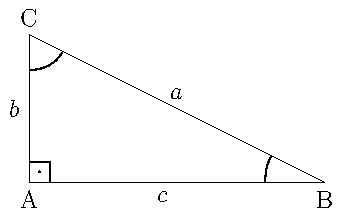
\includegraphics[scale=0.8]{Imagens/fig01.pdf}
        \caption{triângulo retângulo ($\Delta ABC$)}
        \label{fig:01}
    \end{figure}

    \begin{itemize}
        \item O lado BC do $\Delta ABC$ é chamado de hipotenusa e mede a
        \item 	O lado AC do $\Delta ABC$ é chamado de cateto oposto ao ângulo $\hat{B}$ mede b. Este mesmo lado é chamado de cateto adjacente ao ângulo $\hat{C}$
        \item O lado AB do $\Delta ABC$ é chamado de cateto oposto ao ângulo $\hat{C}$ e mede c. Este mesmo lado é chamado de cateto adjacente ao ângulo $\hat{B}$.
    \end{itemize}

Tem-se, por definição, que:

\begin{tcolorbox}[colback=white,colframe=minha_cor,coltitle=black,title=Definição de seno] 
\begin{equation}
    \sen \hat{B} = \df{\text{medida do cateto oposto à } \hat{B}}{\text{medida da hipotenusa}} = \df{b}{a}
    \label{eq:01}
\end{equation}
\end{tcolorbox}

\begin{tcolorbox}[colback=white,colframe=minha_cor,coltitle=black,title=Definição de cosseno] 
\begin{equation}
    \cos \hat{B} = \df{\text{medida do cateto adjacente à } \hat{B}}{\text{medida da hipotenusa}}  = \df{c}{a}
    \label{eq:02}
\end{equation}
\end{tcolorbox}

\begin{tcolorbox}[colback=white,colframe=minha_cor,coltitle=black,title=Definição de cosseno] 
\begin{equation}
    \tg \hat{B} = \df{\text{medida do cateto oposto à } \hat{B}}{\text{medida do cateto adjacente à } \hat{B}} = \df{b}{c}
    \label{eq:03}
\end{equation}
\end{tcolorbox}


Três ângulos muito utilizados em problemas matemáticos envolvendo triângulos retângulos são os ângulos de $30 \degree$, $45 \degree$ e $60 \degree$. Eles são chamados de ângulos notáveis. A partir do triângulo ABC e do quadrado ABCD ilustrados na Figura \ref{fig:02}, é possível calcular o valor de seno, cosseno e tangente dos ângulos notáveis.

\begin{figure}[h]
        \centering
        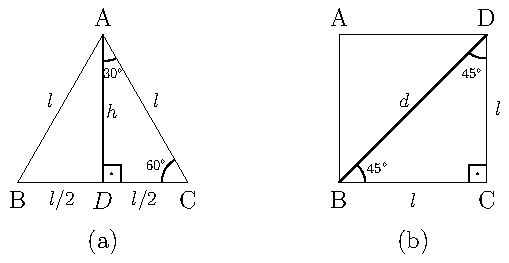
\includegraphics[scale=1.4]{Imagens/fig02.pdf}
        \caption{triângulo (a) e quadrado (b) utilizados para calcular o valor de seno, cosseno e tangente dos ângulos de 30°, 45° e 60° (ângulos notáveis).}
        \label{fig:02}
    \end{figure}

É possível calcular o seno de $30 \degree$ utilizando a fórmula do seno apresentada na equação \ref{eq:01}:
\[
\sen 30 \degree = \dfrac{\frac{l}{2}}{l} = \dfrac{l}{2} \cdot \dfrac{1}{l} = \dfrac{1}{2}
\]

Antes de calcular o cosseno e a tangente de $30 \degree$, é necessário  calcular a altura $h$ do $\Delta ABC$. Para isso, usa-se o teorema de Pitágoras:
\[
l^2 = h^2 + \left(\dfrac{l}{2}\right)^2 \Rightarrow l^2 = h^2 + \dfrac{l^2}{4} \Rightarrow h^2 = \dfrac{3l^2}{4} \Rightarrow h = \dfrac{l\sqrt{3}}{2}.
\]

Em seguida, é possível calcular o cosseno e a tangente de $30 \degree$ através das equações \ref{eq:02} e \ref{eq:03}, respectivamente:

\[
\cos 30 \degree = \dfrac{h}{l} = \dfrac{\dfrac{l\sqrt{3}}{3}}{l} =  \dfrac{l\sqrt{3}}{2} \cdot \dfrac{1}{l} = \dfrac{\sqrt{3}}{2} \; \text{e} \; \tg 30 \degree = \dfrac{\dfrac{l}{2}}{h} =  \dfrac{\dfrac{l}{2}}{\dfrac{l\sqrt{3}}{2}} = \dfrac{l}{2} \cdot \dfrac{2}{l\sqrt{3}} = \dfrac{1}{\sqrt{3}} = \dfrac{\sqrt{3}}{3}
\]

Procedimento análogo pode ser realizado para calcular os valores de seno, cosseno e tangente de $45 \degree$, considerando o quadrado ABCD, e $60 \degree$, considerando o triângulo ABC. A Tabela \ref{tab:01} apresenta os valores de seno, cosseno e tangente dos ângulos notáveis.

%%%%%%%%%%%% TABELA ÂNGULOS NOTÁVEIS %%%%%%%%%%%%
\begin{center}
 %{\fontfamily{helvet}\selectfont Valores de seno, cosseno e tangente de ângulos notáveis.}
 \end{center}
 \vspace{-0.2cm}
\begin{table}[!h]
    \centering     
    \caption{Valores de seno, cosseno e tangente de ângulos notáveis.}
    \begin{tabular}{p{0.12\textwidth}p{0.12\textwidth}p{0.12\textwidth}p{0.12\textwidth}}
\hline
 \begin{center}
     $\alpha$
 \end{center} 
 & 
 \begin{center}
     $\sen \alpha$ 
 \end{center}
 & 
 \begin{center}
     $\cos \alpha$ 
 \end{center}
 & 
 \begin{center}
     $\tg \alpha$
 \end{center}
 \\[-0.4cm]
\hline
 \begin{center}
     $30 \degree$ 
 \end{center}
 & 
 \begin{center}
     $\df{1}{2}$ 
 \end{center}
 & 
 \begin{center}
     $\df{\sqrt{3}}{2}$ 
 \end{center}
 & 
 \begin{center}
     $\df{\sqrt{3}}{3}$
 \end{center}\\[0.35cm]
 \begin{center}
     $45 \degree$ 
 \end{center}
 & 
 \begin{center}
     $\df{\sqrt{2}}{2}$ 
 \end{center}
 & 
 \begin{center}
     $\df{\sqrt{2}}{2}$ 
 \end{center}
 & 
 \begin{center}
     $1$ 
 \end{center}\\[0.35cm]
 \begin{center}
     $60 \degree$
 \end{center} 
 & \begin{center}
     $\df{\sqrt{3}}{2}$
 \end{center} 
 & 
 \begin{center}
     $\df{1}{2}$ 
 \end{center}
 & 
 \begin{center}
     $\sqrt{3}$
 \end{center}\\%[0.15cm]
\hline
\end{tabular}
\label{tab:01}
\end{table}

\subsection{Lei dos senos e lei dos cossenos}

 A lei dos senos e a lei dos cossenos são resultados importantes da trigonometria para estabelecer relações que auxiliam no cálculo dos ângulos e dos lados de triângulos quaisquer (triângulos retângulos, acutângulos e obtusângulos).

\noindent
 \textbf{Lei dos senos:} Em qualquer triângulo ABC (triângulo retângulo ou não), as medidas dos lados são proporcionais aos senos dos ângulos opostos, ou seja,
 $$\df{a}{\sen \hat{A}} = \df{b}{\sen \hat{B}} = \df{c}{\sen \hat{C}}$$

\noindent
\textbf{Exercício Resolvido}

Em um triângulo isósceles, tem-se a base medindo 9 cm e o ângulo oposto a base medindo $120 \degree$. Calcule a medida dos lados congruentes do triângulo.\\

\begin{tikzpicture}[x=0.75pt,y=0.75pt,yscale=-0.65,xscale=0.65]

\draw   (343.49,20.56) -- (490,109.88) -- (190,109.88) -- cycle ;
%Shape: Arc [id:dp8670513073235429] 
\draw  [draw opacity=0] (358.59,29.81) .. controls (355.84,36.02) and (349.03,39.99) .. (341.63,39.1) .. controls (335.6,38.38) and (330.72,34.63) .. (328.46,29.66) -- (343.49,23.56) -- cycle ; \draw   (358.59,29.81) .. controls (355.84,36.02) and (349.03,39.99) .. (341.63,39.1) .. controls (335.6,38.38) and (330.72,34.63) .. (328.46,29.66) ;  
%Shape: Arc [id:dp6736551053433504] 
\draw  [draw opacity=0] (451.18,109.7) .. controls (449.44,106.76) and (448.58,103.21) .. (448.94,99.48) .. controls (449.4,94.83) and (451.66,90.82) .. (454.92,88.14) -- (464.52,101) -- cycle ; \draw   (451.18,109.7) .. controls (449.44,106.76) and (448.58,103.21) .. (448.94,99.48) .. controls (449.4,94.83) and (451.66,90.82) .. (454.92,88.14) ;  
%Shape: Arc [id:dp020705992733369705] 
\draw  [draw opacity=0] (225.63,89.28) .. controls (228.49,91.15) and (230.83,93.95) .. (232.16,97.45) .. controls (233.81,101.82) and (233.56,106.42) .. (231.83,110.27) -- (217.52,103) -- cycle ; \draw   (225.63,89.28) .. controls (228.49,91.15) and (230.83,93.95) .. (232.16,97.45) .. controls (233.81,101.82) and (233.56,106.42) .. (231.83,110.27) ;  

% Text Node
\draw (235,86) node [anchor=north west][inner sep=0.75pt]   [align=left] {$30 \degree$};
% Text Node
\draw (403,86) node [anchor=north west][inner sep=0.75pt]   [align=left] {$30 \degree$};
% Text Node
\draw (322,43) node [anchor=north west][inner sep=0.75pt]   [align=left] {$120  \degree$};
% Text Node
\draw (253,41) node [anchor=north west][inner sep=0.75pt]   [align=left] {x};
% Text Node
\draw (336,118) node [anchor=north west][inner sep=0.75pt]   [align=left] {9};
\end{tikzpicture}
\hfill
\begin{minipage}{8.2cm}
\vspace{-1.5cm}

\noindent
Pela lei dos senos, temo:\\
\[
\frac{9}{\sen 120 \degree}=\frac{x}{\sen 30 \degree}=\frac{x}{\frac{\sqrt{3}}{2}}=\frac{x}{\frac{1}{2}}\Rightarrow x=3 \sqrt{3} \text{cm}
\]
\end{minipage}

\noindent
\textbf{Lei dos cossenos:} Em qualquer triângulo ABC (triângulo retângulo ou não), o quadrado da medida de um lado é igual à soma dos quadrados das medidas dos outros lados menos duas vezes o produto das medidas desses lados pelo cosseno do ângulo que eles formam, ou seja,

$$a^2 = b^2 + c^2 -2bc\cdot\cos\hat{A}$$
$$b^2 = a^2 + c^2 -2ac\cdot\cos\hat{B}$$
$$c^2 = a^2 + b^2 -2ab\cdot\cos\hat{C}$$

\noindent
\textbf{Exercício resolvido} \\
\begin{minipage}{0.5\textwidth}
    Determine a medida de a no triângulo ilustrado na figura a seguir.
\end{minipage}
\vspace{1cm}
\begin{minipage}{0.5\textwidth}
\vspace{1cm}
\centering
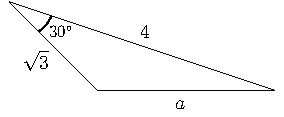
\includegraphics[width=0.8\textwidth]{Imagens/fig04.pdf}
\end{minipage}
Resolução:
\[
a^2=b^2+c^2-2 \cdot b \cdot c \cdot \cos \hat{A} = 4^2+(\sqrt{3})^2-2 \cdot 4 \cdot \sqrt{3} \cdot \cos 30 \degree = 16 + 3 -8 \sqrt{3} \cdot \dfrac{\sqrt{3}}{2}=7
\]
\[
\Rightarrow a=\sqrt{7}
\]

\subsection{Arcos e ângulos}

Algumas definições para o estudo de trigonometria na circunferência são fornecidas a seguir.\\
\begin{center}
\begin{minipage}{6cm}
        \centering
            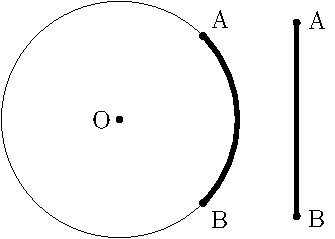
\includegraphics[width=1.2\textwidth]{Imagens/fig05.pdf}
            \captionof{figure}{O arco $\wideparen{AB}$ e comprimento desse arco dado pela medida algébrica do segmento $\overline{AB}$.}
            \label{fig:fig05}
\end{minipage}
\end{center}

\noindent
\textbf{Arco geométrico:} é uma das partes da circunferência delimitada por dois pontos, incluindo-os.

\noindent
\textbf{Comprimento de um arco:} é o comprimento do segmento de reta que se obtém ao “desentortar” (ou retificar) o arco. Conhecendo o raio da circunferência e a medida em graus do arco, o comprimento do arco pode ser calculado através de uma regra de três simples:\\

\begin{center}
\begin{tabular}{rcl}
Graus    &        & Comprimento do arco   \\
$360$    & ------ & $2 \pi r$      \\
$\alpha$ & ------ & $x$        \\
\end{tabular}
\end{center}

Nesse caso, o comprimento $x$ é expresso na mesma unidade do raio da circunferência. Em uma circunferência de raio $r=1$, a regra de três acima é simplificada da seguinte forma:

\begin{center}
\begin{tabular}{rcl}
Graus    &        & Comprimento do arco   \\
$180$    & ------ & $\pi$      \\
$\alpha$ & ------ & $x$        \\
\end{tabular}
\end{center}

\noindent
\textbf{Medida em radianos:} Observe na Figura \ref{fig:fig06} que os arcos $\wideparen{AB}$, $\wideparen{CD}$ e $\wideparen{EF}$ têm a mesma medida em graus, porém têm comprimentos diferentes. Utilizando a regra de três acima, tem-se que:

\begin{minipage}{5cm}
    \[
    x_1=\dfrac{\pi r_1}{6} \;\;\; x_2=\dfrac{\pi r_2}{6} \;\;\; x_3=\dfrac{\pi r_3}{6}
    \]
\end{minipage}
\hfill
\begin{minipage}{8cm}
        \centering
            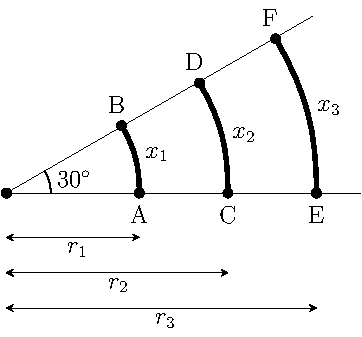
\includegraphics[width=0.8\textwidth]{Imagens/fig06.pdf}
            \captionof{figure}{Arco com raios diferentes.}
            \label{fig:fig06}
\end{minipage}

\vspace{1cm}
Note que $\dfrac{x_1}{r_1}=\dfrac{x_2}{r_2}=\dfrac{x_3}{r_3}=\dfrac{\pi}{6}$. A razão entre o comprimento do arco e o raio, que nesse exemplo é $\dfrac{\pi}{6}$, é a \textbf{medida em radianos} do arco (e também do ângulo central).

\subsection{Circunferência trigonométrica}
Passa-se a utilizar a circunferência unitária (ou circunferência trigonométrica), uma circunferência com raio igual a 1 unidade de comprimento associada a um sistema de coordenadas cartesianas ortogonais rOs, conforme a Figura \ref{fig:fig07e08} (a). Os pontos A,B,C e D, intersecções da circunferência trigonométrica com os eixos coordenados, dividem a circunferência em quatro partes congruentes denominadas \textbf{quadrantes}.

\begin{minipage}{13.5cm}
     \centering
\begin{minipage}{6cm}
     \centering
            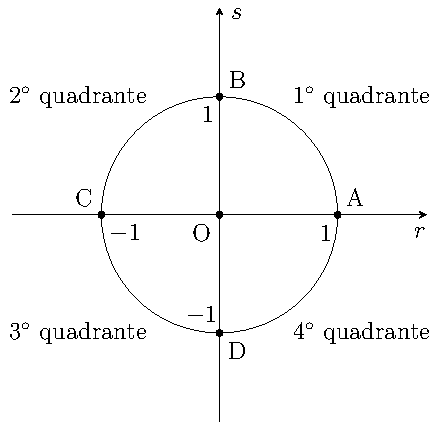
\includegraphics[width=\textwidth]{Imagens/fig07.pdf}
\end{minipage}
\hfill
\begin{minipage}{6cm}
        \centering
            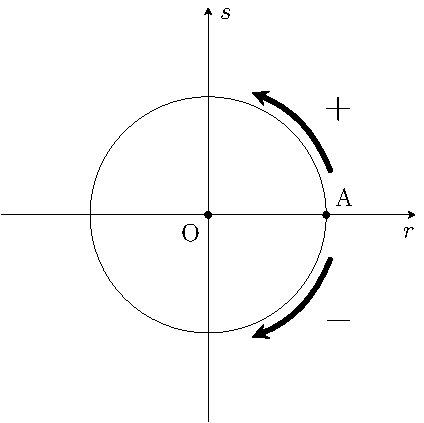
\includegraphics[width=\textwidth]{Imagens/fig08.pdf}
\end{minipage}
\captionof{figure}{Circunferência trigonométrica e seus quadrantes (a); sentidos da circunferência trigonométrica (b).}
\label{fig:fig07e08}
\end{minipage}


Podemos associar a cada número real $x$ um ponto da circunferência trigonométrica. Ao número $x=0$, associamos o ponto A. Se $x \neq 0$, associamos a $x$ o ponto final $P$ do seguinte percurso de comprimento igual a $|x|$ realizado sobre a circunferência partindo de $A$, de acordo com a Figura \ref{fig:fig07e08} (b):

\begin{itemize}
    \item 	Se $x>0$, percorremos a circunferência trigonométrica no sentido anti-horário;
    \item 	Se $x<0$, percorremos a circunferência trigonométrica no sentido horário.
\end{itemize}

O ponto $P$ associado à $x$ é denominado \textbf{imagem de $x$} na circunferência trigonométrica e o arco $\wideparen{AP}$ tem $x$ rad.

\noindent
\textbf{Exercício Resolvido:} Marcar na circunferência trigonométrica a imagem do número $x$ em cada caso:

\begin{tasks}(4)
    \task $x=\dfrac{\pi}{2}$
    \task $x=1$
    \task $x=-1$
    \task $x=-\dfrac{2 \pi}{3}$
\end{tasks}
\noindent
Resolução:\\
\begin{minipage}{\textwidth}
     \centering
\begin{minipage}{0.24\textwidth}
     \centering
            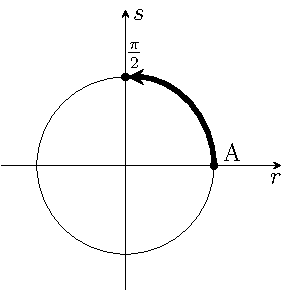
\includegraphics[width=\textwidth]{Imagens/fig09.pdf}
\end{minipage}
\begin{minipage}{0.24\textwidth}
        \centering
            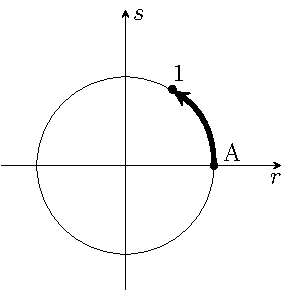
\includegraphics[width=\textwidth]{Imagens/fig10.pdf}
\end{minipage}
\begin{minipage}{0.24\textwidth}
     \centering
            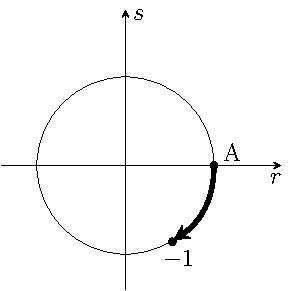
\includegraphics[width=\textwidth]{Imagens/fig11.pdf}
\end{minipage}
\begin{minipage}{0.24\textwidth}
        \centering
            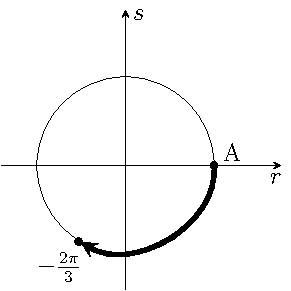
\includegraphics[width=\textwidth]{Imagens/fig12.pdf}
\end{minipage}
\end{minipage}

Se o ponto da circunferência, final do arco iniciado em (1,0), é o mesmo para dois arcos diferentes, então chamamos estes arcos de \textbf{arcos côngruos} (ou congruentes). Observe que todos os arcos côngruos diferem si de um múltiplo de $2\pi$ rad (ou $360\degree$), que é o comprimento de cada volta. Dessa forma, os arcos ($x+k \cdot 2\pi$) rad (ou $\alpha+k \cdot 360\degree$), para $k \in \mathbb{Z}$, são côngruos.\\

\noindent
\textbf{Exercício Resolvido:} Dentre os arcos abaixo, identifique os côngruos:

\begin{tasks}(2)
    \task $30 \degree \;\; \text{e} \;\; 330 \degree$
    \task $\dfrac{\pi}{3} \text{rad} \;\; \text{e} \;\; \dfrac{31 \pi}{3} \text{rad}  $
\end{tasks}
\noindent
Resolução:\\
 
\begin{tasks}
    \task 	Encontrar $k \in \mathbb{Z}$, tal que $30 + k \cdot 360 \degree = 330 \degree \Rightarrow k = \dfrac{5}{6} \not \in Z \Rightarrow 30 \degree$ e $330 \degree$ não são côngruos.
    \task 	Encontrar $k \in \mathbb{Z}$, tal que $\dfrac{\pi}{3} + 2k \pi = \dfrac{31 \pi}{3} \Rightarrow k = 5 \in Z \Rightarrow \dfrac{\pi}{3} \text{rad e }\dfrac{31 \pi}{3} \text{rad}$ são côngruos.
\end{tasks}

\subsection{Seno e cosseno na circunferência trigonométrica}

Dado  $x \in \mathbb{R}$ com imagem de $x$ na circunferência trigonométrica sendo um ponto com coordenadas $(a,b)$, definimos:

\begin{tcolorbox}[colback=white,colframe=minha_cor,coltitle=black,title=Definição: Seno e cosseno] 
\[
\cos x = a \text{  e  } \sen x = b
\]
\end{tcolorbox}

Dessa forma, passa-se a chamar o eixo das abscissas de \textbf{eixo dos cossenos} e o eixo das ordenadas de \textbf{eixo dos senos}, conforme a Figura \ref{fig:fig13}.
\begin{center}
    \begin{minipage}{7cm}
        \centering
            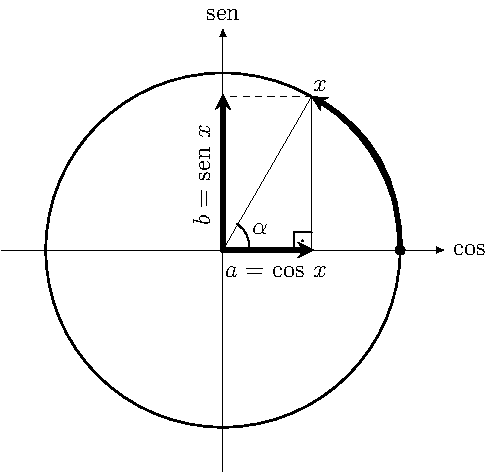
\includegraphics[width=1.2\textwidth]{Imagens/fig13.pdf}
            \captionof{figure}{Circunferência trigonométrica e sua relação com seno e cosseno de um número real $x$.}
            \label{fig:fig13}
    \end{minipage}
\end{center}

Nota-se que as definições de seno e cosseno de um ângulo agudo em um triângulo retângulo são coerentes com as definições na circunferência trigonométrica:
\[
\sen \alpha = \dfrac{\text{medida do cateto oposto}}{\text{medida da hipotenusa}} = \dfrac{b}{1} = b = \sen x
\]
\[
\cos \beta = \dfrac{\text{medida do cateto adjacente}}{\text{medida da hipotenusa}} = \dfrac{a}{1} = a = \cos x
\]

Os valores de seno e cosseno das medidas de arcos dadas em graus são iguais aos valores de seno e cosseno dos números reais que se obtêm transformando essas medidas em radianos.

Além disso, utilizando propriedades de simetria em relação aos eixos coordenados, obtém-se os arcos e seus correspondentes valores de seno e cosseno, conforme a circunferência trigonométrica apresentada na Figura \ref{fig:fig05_circtrigcompl}.

\begin{figure}[h]
        \centering
        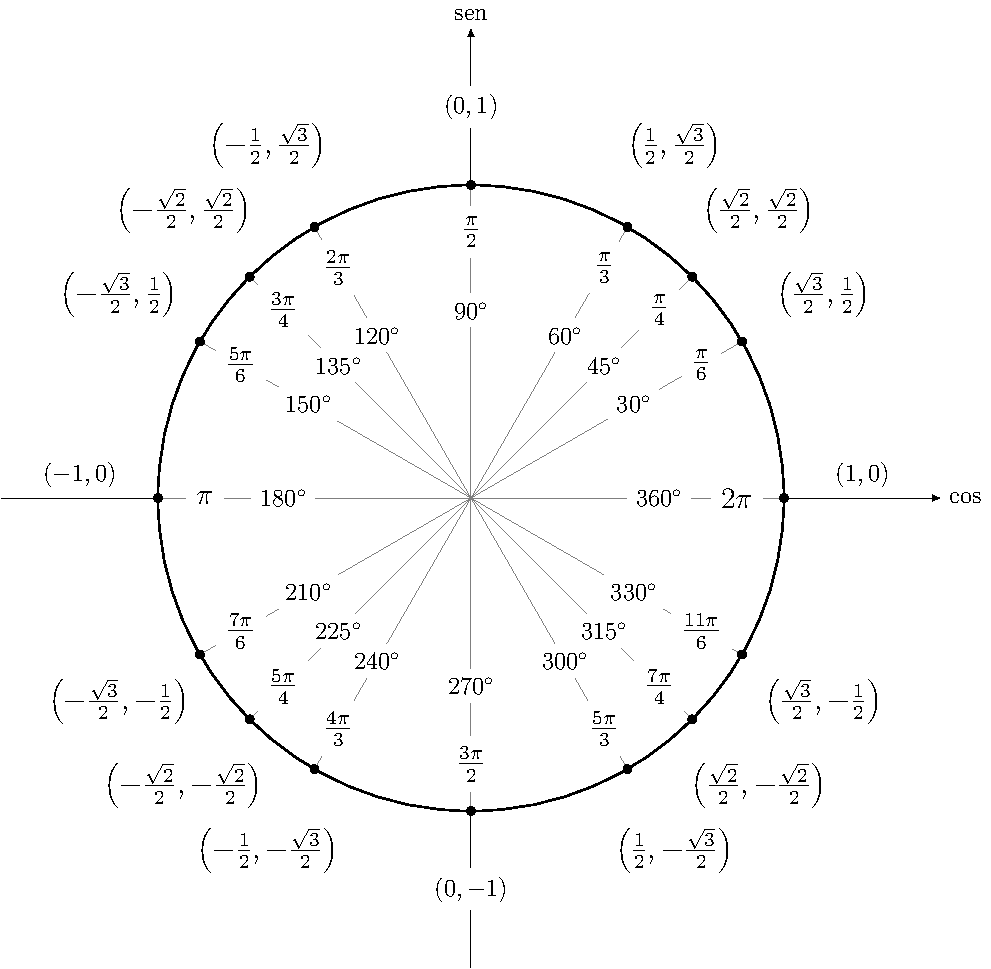
\includegraphics[width=\textwidth]{Imagens/fig05_circtrigcompl.pdf}
        \caption{Circunferência trigonométrica com os principais arcos (em graus e em radianos) e seus correspondentes valores de seno e cosseno apresentados em pares de coordenadas.}
        \label{fig:fig05_circtrigcompl}
 \end{figure}

Nota-se que dois arcos côngruos possuem senos iguais e cossenos iguais. Em outras palavras, para todo $x \in \mathbb{R}$ e para todo $k \in \mathbb{Z}$, temos:
\[
\sen (x + 2 k \pi) = \sen x
\]
\[
\cos (x + 2 k \pi) = \cos x
\]

\noindent
\textbf{Exercício resolvido} 

Calcule o valor da expressão
\[
\dfrac{\cos \dfrac{7 \pi}{6}-\sen \dfrac{\pi}{3}}{\sen \left(-\dfrac{\pi}{4}\right) + \cos \dfrac{19 \pi}{3}}
\]

\noindent
Resolução:
\[
\dfrac{\cos \dfrac{7 \pi}{6}-\sen \dfrac{\pi}{3}}{\sen \left(-\dfrac{\pi}{4}\right) + \cos \dfrac{19 \pi}{3}} = \dfrac{- \dfrac{\sqrt{3}}{2} - \dfrac{\sqrt{3}}{2}}{- \dfrac{\sqrt{2}}{2} + \dfrac{1}{2}} = \dfrac{- 2 \sqrt{3}}{1 - \sqrt{2}} = \dfrac{ 2 \sqrt{3}}{\sqrt{2}-1} \cdot \dfrac{\sqrt{2}+1}{\sqrt{2}+1} = 2 \sqrt{6} + 2 \sqrt{3}
\]
\textbf{Tangente na circunferência trigonométrica}

Pelo ponto $A$, origem da circunferência trigonométrica, a reta $t$ paralela ao eixo dos senos é traçada e orientada no mesmo sentido dele. Dado um número real $x$ com imagem no ponto $P$ da circunferência trigonométrica, tal que a reta $\overleftrightarrow{OP}$ intercepta o eixo das tangentes no ponto $T$, define-se $\tg x$ a medida algébrica do segmento $\overline{AT}$, que será positiva quando $T$ estiver “acima” de $A$, e negativa quando $T$ estiver “abaixo” de $A$. Dessa forma, passa-se a chamar a reta $t$ de \textbf{eixo das tangentes}, conforme a Figura \ref{fig:fig14}.
\begin{center}
    \begin{minipage}{10cm}
        \centering
            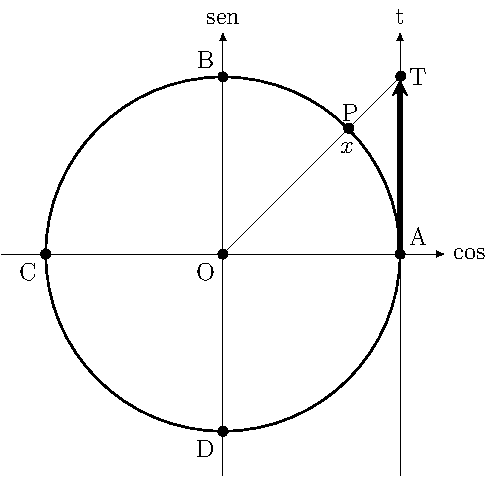
\includegraphics[width=0.7\textwidth]{Imagens/fig14.pdf}
            \captionof{figure}{Circunferência trigonométrica com o eixo das tangentes.}
            \label{fig:fig14}
    \end{minipage}
\end{center}

Observe que, quando $P=B$ ou $P=D$, a reta $\overleftrightarrow{OP}$ é paralela ao eixo das tangentes e, portanto, não existe o ponto $T$. Nesse caso, não existe $\tg x$. Então,
\[
x \neq \dfrac{(2 k + 1) \pi}{2}, \;\; k \in \mathbb{Z} \Longrightarrow  \exists \tg x 
\]
\section{Funções trigonométricas}	

A seguir, os conceitos visto até aqui serão formalizados sob o ponto de vista de funções matemáticas.

\subsection{Estudo da função seno}

Dado um número real $x$, associa-se a ele o valor do seno de um arco de $x$ radianos. Assim, define-se a função seno como a função real de variável real que associa a cada número real $x$ o valor real $\sen x$, ou seja,
\begin{center}
    \begin{tabular}{llll}
    $f:$ & $\mathbb{R}$ & $\rightarrow$ & $\mathbb{R}$\\
    & $x$ & $\mapsto$ & $f(x) = \sen x$\\
\end{tabular}    
\end{center}

A partir de valores de $x$ da primeira volta positiva na circunferência trigonométrica (esses valores foram apresentados anteriormente na Figura \ref{fig:fig05_circtrigcompl}), constrói-se o gráfico da função seno apresentado abaixo. %na Figura \ref{fig:fig16}.

%\begin{center}
%    \begin{minipage}{14cm}
%        \centering
%            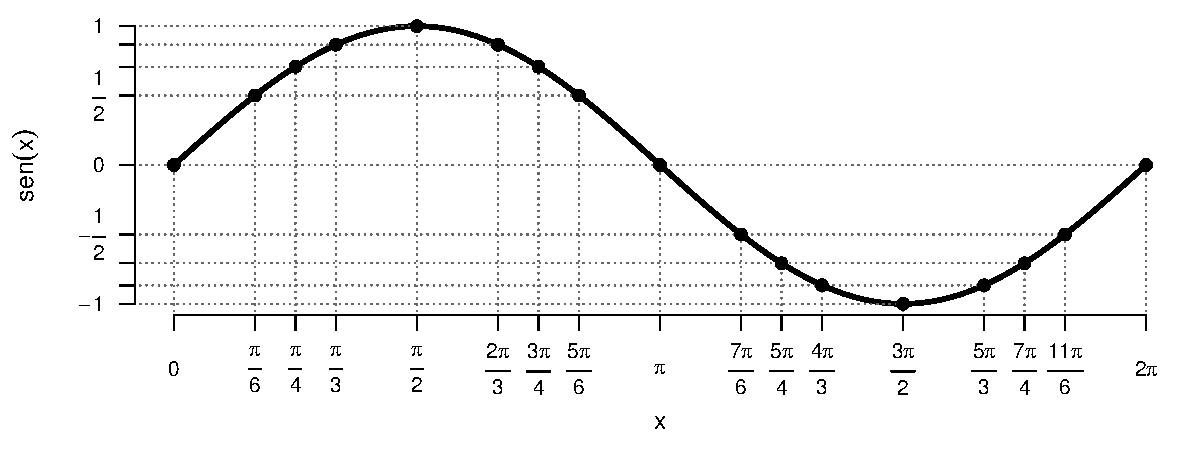
\includegraphics[width=\textwidth]{Imagens/fig16.pdf}
%            \captionof{figure}{Gráfico da função seno para $x \in [0,2 \pi]$.}
%            \label{fig:fig16}
%    \end{minipage}
%\end{center}


%%%%%%%%%%%%%%%%%%%%%%%%%%%%%%%%%%%%%%	
\begin{center}
\begin{tikzpicture}
\begin{axis}[
width=0.8\textwidth,
xlabel=$x$,
ylabel=$y$,
title={Gráfico da função seno para $x \in [0,2 \pi]$.},
axis lines=middle,
xmin=0,
xmax=2*pi,
ymin=-1,
ymax=1,
xtick={0,pi/6,pi/3,pi/2,2*pi/3,5*pi/6,pi,7*pi/6,4*pi/3,3*pi/2,5*pi/3,11*pi/6,2*pi},
xticklabels={$0$,$\frac{\pi}{6}$,$\frac{\pi}{3}$,$\frac{\pi}{2}$,$\frac{2\pi}{3}$,$\frac{5\pi}{6}$,$\pi$,$\frac{7\pi}{6}$,$\frac{4\pi}{3}$,$\frac{3\pi}{2}$,$\frac{5\pi}{3}$,$\frac{11\pi}{6}$,$2\pi$},
ytick={-1,-0.5,0,0.5,1},
enlargelimits,
ticks=both,
tick label style={font=\footnotesize},
after end axis/.code={
\draw (axis cs:0,\pgfkeysvalueof{/pgfplots/ymin}) -- (axis cs:0,\pgfkeysvalueof{/pgfplots/ymax});
\draw (axis cs:\pgfkeysvalueof{/pgfplots/xmin},0) -- (axis cs:\pgfkeysvalueof{/pgfplots/xmax},0);
\node[black, above right] at (axis cs:2.8,0.5) {$y =\sin(x)$};
}
]
\addplot[domain=0:2*pi, blue, samples=100] {sin(deg(x))};
\end{axis}
\end{tikzpicture}
\end{center}


            



Nota-se que a função seno é definida no conjunto dos números reais. Assim, a curva pode ser estendida para valores de $x$ menores do que 0 e maiores do que $2 \pi$.

\textbf{Observações sobre a função seno:}
\begin{itemize}
    \item 	O domínio de $f(x)= \sen x$ é $D(f) = \mathbb{R}$, pois para qualquer valor real de $x$ existe um e, somente um, valor para $\sen x$.
    \item   O conjunto imagem de $f(x)= \sen x$ é o intervalo $[-1,1]$.
    \item   A função seno não é sobrejetiva, pois sua imagem não é igual ao contradomínio, isto é, $Im(f)=[-1,1] \neq \mathbb{R} = CD(f)$.
    \item   A função seno não é injetiva, pois, para valores diferentes de $x$, temos o mesmo $f(x)$.
    \item   A função seno é uma função ímpar, isto é, qualquer que seja $x \in D(f) = \mathbb{R} $, tem-se que $\sen x = - \sen (-x)$.
    \item   A função seno é periódica com período igual à $ 2 \pi$, isto é, $\sen x = \sen (x+2k \pi)$, com $k \in \mathbb{R} e x \in \mathbb{R}$.
\end{itemize}
\subsection{Estudo da função cosseno}

Dado um número real $x$, associa-se a ele o valor do cosseno de um arco de $x$ radianos. Assim, a função cosseno é definida como a função real de variável real que associa a cada número real $x$ o valor real $\cos x$, ou seja,
\begin{center}
\begin{tabular}{llll}
$f:$ & $\mathbb{R}$ & $\rightarrow$ & $\mathbb{R}$\\
   & $x$ & $\mapsto$ & $f(x) = \cos x$\\
\end{tabular}
\end{center}

A partir de valores de $x$ da primeira volta positiva na circunferência trigonométrica (esses valores foram apresentados anteriormente na Figura \ref{fig:fig05_circtrigcompl}), constrói-se o gráfico da função cosseno apresentado abaixo. %na Figura \ref{fig:fig17}.
%\begin{center}
%    \begin{minipage}{14cm}
%        \centering
%            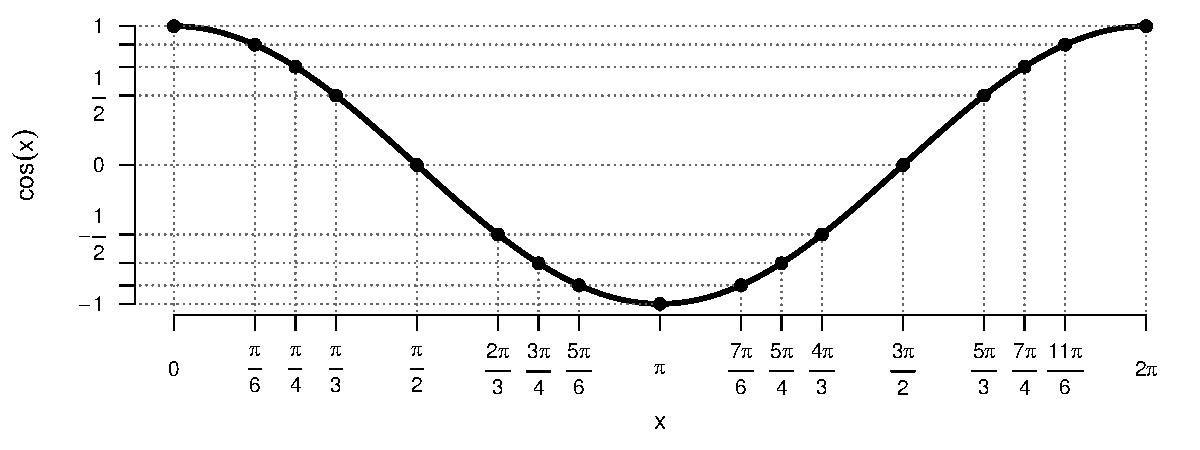
\includegraphics[width=\textwidth]{Imagens/fig17.pdf}
%            \captionof{figure}{Gráfico da função cosseno para $x %\in [0,2 \pi]$.}
%            \label{fig:fig17}
%    \end{minipage}
%\end{center}

%%%%%%%%%%%%%%%%%%%%%%%%%%%%%%%%%%%%%%	
\begin{center}
\begin{tikzpicture}
\begin{axis}[
width=0.8\textwidth,
xlabel=$x$,
ylabel=$y$,
title={Gráfico da função cosseno para $x \in [0,2 \pi]$.},
axis lines=middle,
xmin=0,
xmax=2*pi,
ymin=-1,
ymax=1,
xtick={0,pi/6,pi/3,pi/2,2*pi/3,5*pi/6,pi,7*pi/6,4*pi/3,3*pi/2,5*pi/3,11*pi/6,2*pi},
xticklabels={$0$,$\frac{\pi}{6}$,$\frac{\pi}{3}$,$\frac{\pi}{2}$,$\frac{2\pi}{3}$,$\frac{5\pi}{6}$,$\pi$,$\frac{7\pi}{6}$,$\frac{4\pi}{3}$,$\frac{3\pi}{2}$,$\frac{5\pi}{3}$,$\frac{11\pi}{6}$,$2\pi$},
ytick={-1,-0.5,0,0.5,1},
enlargelimits,
ticks=both,
tick label style={font=\footnotesize},
after end axis/.code={
\draw (axis cs:0,\pgfkeysvalueof{/pgfplots/ymin}) -- (axis cs:0,\pgfkeysvalueof{/pgfplots/ymax});
\draw (axis cs:\pgfkeysvalueof{/pgfplots/xmin},0) -- (axis cs:\pgfkeysvalueof{/pgfplots/xmax},0);
\node[black, above right] at (axis cs:1.1,0.5) {$y =\cos(x)$};
}
]
\addplot[domain=0:2*pi, blue, samples=100] {cos(deg(x))};
\end{axis}
\end{tikzpicture}
\end{center}


Similarmente à função seno, a curva da função cosseno pode ser estendida para valores de $x$ menores do que 0 e maiores do que $2 \pi$.

\textbf{Observações sobre a função cosseno:}
\begin{itemize}
   \item O domínio e a imagem da função cosseno são os mesmos da função seno.
    \item Assim como a função seno, a função cosseno não é nem sobrejetiva nem injetiva.
    \item A função cosseno é uma função par, isto é, qualquer que seja $x\in \text{D}(f)$, temos que $\cos x= \cos (-x)$.
    \item A função cosseno é periódica com período igual à $2\pi$.
\end{itemize}

\subsection{Estudo da função tangente}

Define-se função tangente como a função real de variável real que associa a cada número $x$ o valor $\tg x$, desde que $x$ não seja $\frac{\pi}{2}$ nem $\frac{3\pi}{2}$ e nenhum de seus respectivos arcos côngruos, isto é,

\begin{center}
\begin{tabular}{llll}
$f:$ & $\mathbb{D}$ & $\rightarrow$ & $\mathbb{R}$\\
   & $x$ & $\mapsto$ & $f(x) = \tg x$\\
\end{tabular}
\end{center}
em que $\mathbb{D} = \left\{x \in \mathbb{R} \ | \ x \neq \df{(2k+1)\pi}{2}, \text{com} \ k \in \mathbb{Z}\right\}$

A partir de valores de $x$ da primeira volta positiva na circunferência trigonométrica (esses valores foram apresentados anteriormente na Figura \ref{fig:fig05_circtrigcompl}), constrói-se o gráfico da função tangente apresentado abaixo. % na Figura \ref{fig:fig18}.
%\begin{center}
%    \begin{minipage}{14cm}
%        \centering
%            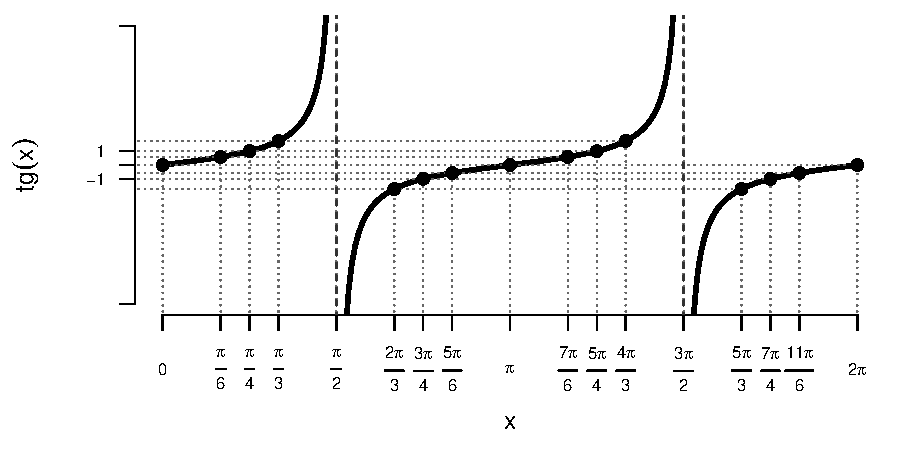
\includegraphics[width=\textwidth]{Imagens/fig18.pdf}
%            \captionof{figure}{Gráfico da função tangente para $x \in [0,2 \pi]$.}
%            \label{fig:fig18}
%    \end{minipage}
%\end{center}

%%%%%%%%%%%%%%%%%%%%%%%%%%%%%%%%%%%%%%%%%%%%%%%%
\begin{center}
\begin{tikzpicture}
\begin{axis}[
restrict y to domain=-10:10,
samples=1000,
% some fine-tuning for the display:
width=17cm, height=220pt,
xlabel=$x$,
ylabel=$\tg(x)$,
title={Gráfico da função tangente para $x \in [-2 \pi,2 \pi]$.},
xmin=-2.2*pi, xmax=2.2*pi,
xtick={-2*pi,-3*pi/2,...,2*pi},
xticklabels={$-2\pi$,$-\frac{11\pi}{6}$,$-\frac{5\pi}{3}$,$-\frac{3\pi}{2}$,$-\frac{4\pi}{3}$,$-\pi$,$\frac{7\pi}{6}$,$-\frac{5\pi}{6}$,$-\frac{2\pi}{3}$,$-\frac{\pi}{2}$,$-\frac{\pi}{3}$,$-\frac{\pi}{6}$,$0$,$\frac{\pi}{6}$,$\frac{\pi}{3}$,$\frac{\pi}{2}$,$\frac{2\pi}{3}$,$\frac{5\pi}{6}$,$\pi$,$\frac{7\pi}{6}$,$\frac{4\pi}{3}$,$\frac{3\pi}{2}$,$\frac{5\pi}{3}$,$\frac{11\pi}{6}$,$2\pi$},
axis x line=center,
axis y line=center,
]
\addplot [blue] gnuplot [id=tangens,domain=-2*pi:2*pi] {tan(x)};
\draw[dashed] (-3*pi/2,-10) -- (-3*pi/2,10);
\draw[dashed] (-pi/2,-10) -- (-pi/2,10);
\draw[dashed] (pi/2,-10) -- (pi/2,10);
\draw[dashed] (3*pi/2,-10) -- (3*pi/2,10);
%\legend{$\tan(x)$}
\end{axis}
\end{tikzpicture}
\end{center}
%%%%%%%%%%%%%%%%%%%%%%%%%%%%%%%%%%%%%%%%%%%

Nota-se que à medida que $x$ tende aos valores $\frac{\pi}{2}, \frac{3\pi}{2}$ e seus respectivos arcos côngruos, o gráfico da tangente tende ao infinito (positivo ou negativo). A curva da função tangente pode ser estendida para valores de $x$ menores do que $0$ e maiores do que $2\pi$.

\textbf{Observações sobre a função tangente:}
\begin{itemize}
   \item A função tangente tem $\text{D}(f)=\left\{x \in \mathbb{R} \ | \ x \neq \frac{(2k+1)\pi}{2}, \text{com} \ k \in \mathbb{Z}\right\}$ e $\text{Im}(f)=\mathbb{R}$.
    \item A função tangente não é injetiva, mas é sobrejetiva.
    \item A função tangente é função ímpar, isto é, $\tg x= -\tg (-x),\forall x\in \text{D}(f)$.
    \item A função tangente é periódica com período igual à $\pi$, isto é, $\tg x=\tg (x+k\pi), \text{com} \ k\in \mathbb{Z}$ e $x\in \text{D}(f)$.
\end{itemize}

\section{Relações e transformações trigonométricas}

As relações e transformações trigonométricas são apresentadas a seguir.

\begin{tcolorbox}[colback=white,colframe=minha_cor,coltitle=black,title=Relações trigonométricas] 
    \begin{minipage}{6.5cm}
    \textbf{Relações principais:} \\[0.25cm]
    $\sen^2 x + \cos^2 x = 1$ \\[0.25cm]
    $\tg x = \df{\sen x}{\cos x}, \forall x \neq \df{(2k+1)\pi}{2}$ \\[0.25cm]
    $\cotg x = \df{\cos x}{\sen x}, \forall x \neq k\pi$ \\[0.25cm]
    $\sec x = \df{1}{\cos x}, \forall x \neq \df{(2k+1)\pi}{2}$ \\[0.25cm]
    $\cossec x = \df{1}{\sen x}, \forall x \neq k\pi$
\end{minipage}
\hfill
\begin{minipage}{6.5cm}
    \textbf{Relações decorrentes:} \\[0.25cm]
    $\cotg x = \df{1}{\tg x}, \forall x \neq \df{k\pi}{2}$ \\[0.25cm]
    $\sec^2x = 1 + \tg^2x, \forall x \neq \df{(2k+1)\pi}{2}$ \\[0.25cm]
    $\cossec^2x = 1 + \cotg^2x, \forall x \neq k\pi$\\[1.50cm]
\end{minipage}
\end{tcolorbox}

\begin{tcolorbox}[colback=white,colframe=minha_cor,coltitle=black,title=Soma de diferença de arcos] 
\begin{center}
    \begin{minipage}{6.5cm}
    $\sen (a \pm b) = \sen a \cdot \cos b \pm \sen b \cdot \cos a$ \\[0.25cm]
    $\cos (a \pm b) = \cos a \cdot \cos b \mp \sen a \cdot \cos b$ \\[0.25cm]
    $\tg (a \pm b) = \dfrac{\tg a \pm \tg b}{1 + tg a \cdot \tg b}$ \\
    \end{minipage}
\end{center}
\end{tcolorbox}

\begin{tcolorbox}[colback=white,colframe=minha_cor,coltitle=black,title=Divisão de arcos] 
\begin{center}
    \begin{minipage}{6.5cm}
    $\sen^2 \dfrac{x}{2} = \dfrac{1- \cos x}{2}$ \\[0.25cm]
    $\cos^2 \dfrac{x}{2} = \dfrac{1+ \cos x}{2}$ \\[0.25cm]
    $\tg^2 \dfrac{x}{2} = \dfrac{1- \cos x}{1+ \cos x}$ \\
    \end{minipage}
\end{center}
\end{tcolorbox}

\begin{tcolorbox}[colback=white,colframe=minha_cor,coltitle=black,title=Multiplicação de arcos] 
\begin{center}
    \begin{minipage}{6.5cm}
    $\sen 2a = 2 \cdot \sen a \cdot \cos a$ \\[0.25cm]
    $\cos 2a = \cos^2 a - \sen^2 a$ \\[0.25cm]
    $\tg 2a = \dfrac{2 \cdot \tg a}{1- \tg^2 a}$ \\
    \end{minipage}
\end{center}
\end{tcolorbox}

\begin{tcolorbox}[colback=white,colframe=minha_cor,coltitle=black,title=Transformação em produtos] 
\begin{center}
    \begin{minipage}{7cm}
    $\sen p + \sen q = 2 \cdot \sen \dfrac{p + q}{2} \cdot \cos \dfrac{p - q}{2}$ \\[0.25cm]
    $\sen p - \sen q = 2 \cdot \sen \dfrac{p - q}{2} \cdot \cos \dfrac{p + q}{2}$ \\[0.25cm]
    $\cos p + \cos q = 2 \cdot \cos \dfrac{p + q}{2} \cdot \cos \dfrac{p - q}{2}$ \\[0.25cm]
     $\cos p - \sen q = -2 \cdot \sen \dfrac{p + q}{2} \cdot \sen \dfrac{p - q}{2}$ \\
    \end{minipage}
\end{center}
\end{tcolorbox}

\begin{texample}
        \centering
        \tcbhighmath{\text{Seja } \sen x = \dfrac{2}{5} \text{  e  }  0 < x < \dfrac{\pi}{2}. \text{ Calcule } \cos x \text{  e  } \tg x.}
\end{texample}
Resolução:
\[\sen^2 x + \cos^2 x = 1 \Rightarrow \left(\dfrac{2}{5}\right)^2 + \cos^2 x = 1 \Rightarrow \cos^2 x  = \dfrac{21}{25}\Rightarrow \cos x =  
    \left\{  
         \begin{array}{c}
            \dfrac{-\sqrt{21}}{5} \\[0.3cm]
		  \dfrac{+\sqrt{21}}{5} \\
	\end{array} 
    \right. 
\]
\[
\Rightarrow \cos x = \dfrac{\sqrt{21}}{5} \text{ e } \tg x = \dfrac{\sen x}{\cos x} = \dfrac{\frac{2}{5}}{\frac{\sqrt{21}}{5}} = \dfrac{2 \sqrt{21}}{21}
\]

\begin{texample}
        \centering
        \tcbhighmath{\text{Calcule  valor da expressão } \sen 105 \degree - \cos 75 \degree}
\end{texample}
Resolução:
\[
\Rightarrow 105 \degree = 60 \degree + 45 \degree \text{ e } 75 \degree = 30 \degree + 45 \degree
\]
\[
\sen 105 \degree - \cos 75 \degree = \sen(60 \degree + 45 \degree) - \cos(30 \degree + 45 \degree) =
\]
\[
\dfrac{\sqrt{3}}{2} \cdot \dfrac{\sqrt{2}}{2} + \dfrac{\sqrt{2}}{2} \cdot \dfrac{1}{2} - \left[ \dfrac{\sqrt{3}}{2} \cdot \dfrac{\sqrt{2}}{2} - \dfrac{1}{2} \cdot  \dfrac{\sqrt{2}}{2}  \right] = \dfrac{\sqrt{6}}{4} + \dfrac{\sqrt{2}}{4} - \left[ \dfrac{\sqrt{6}}{4} - \dfrac{\sqrt{2}}{4} \right] =
\]
\[
\dfrac{\sqrt{6}}{4} + \dfrac{\sqrt{2}}{4} -  \dfrac{\sqrt{6}}{4} + \dfrac{\sqrt{2}}{4} =
\dfrac{2 \sqrt{2}}{4} = \dfrac{\sqrt{2}}{4}
\]

 \section{Exercícios}

 \begin{enumerate}
     \item 	Calcular seno, cosseno e tangente dos ângulos de $45 \degree$ e $60 \degree$, conferindo os resultados com os valores da Tabela de ângulos notáveis.
    \item   Esboce a circunferência trigonométrica, indicando os principais arcos em radiano e seus correspondentes valores de seno e cosseno.
    \item   O triângulo isósceles é um tipo de triângulo que possui dois lados iguais e, consequentemente, dois ângulos iguais formados com a base. Observe a figura abaixo e determine a medida dos lados congruentes deste triângulo.
\begin{center}
\begin{tikzpicture}[x=0.75pt,y=0.75pt,yscale=-1,xscale=1]
%uncomment if require: \path (0,300); %set diagram left start at 0, and has height of 300

%Shape: Triangle [id:dp9164804627843453] 
\draw   (343.49,20.56) -- (490,109.88) -- (190,109.88) -- cycle ;
%Shape: Arc [id:dp8670513073235429] 
\draw  [draw opacity=0] (358.59,29.81) .. controls (355.84,36.02) and (349.03,39.99) .. (341.63,39.1) .. controls (335.6,38.38) and (330.72,34.63) .. (328.46,29.66) -- (343.49,23.56) -- cycle ; \draw   (358.59,29.81) .. controls (355.84,36.02) and (349.03,39.99) .. (341.63,39.1) .. controls (335.6,38.38) and (330.72,34.63) .. (328.46,29.66) ;  
%Shape: Arc [id:dp6736551053433504] 
\draw  [draw opacity=0] (451.18,109.7) .. controls (449.44,106.76) and (448.58,103.21) .. (448.94,99.48) .. controls (449.4,94.83) and (451.66,90.82) .. (454.92,88.14) -- (464.52,101) -- cycle ; \draw   (451.18,109.7) .. controls (449.44,106.76) and (448.58,103.21) .. (448.94,99.48) .. controls (449.4,94.83) and (451.66,90.82) .. (454.92,88.14) ;  
%Shape: Arc [id:dp020705992733369705] 
\draw  [draw opacity=0] (225.63,89.28) .. controls (228.49,91.15) and (230.83,93.95) .. (232.16,97.45) .. controls (233.81,101.82) and (233.56,106.42) .. (231.83,110.27) -- (217.52,103) -- cycle ; \draw   (225.63,89.28) .. controls (228.49,91.15) and (230.83,93.95) .. (232.16,97.45) .. controls (233.81,101.82) and (233.56,106.42) .. (231.83,110.27) ;  
% Text Node
\draw (235,86) node [anchor=north west][inner sep=0.75pt]   [align=left] {$30 \degree$};
% Text Node
\draw (403,86) node [anchor=north west][inner sep=0.75pt]   [align=left] {$30 \degree$};
% Text Node
\draw (322,43) node [anchor=north west][inner sep=0.75pt]   [align=left] {$120 \degree$};
% Text Node
\draw (253,41) node [anchor=north west][inner sep=0.75pt]   [align=left] {$x$};
% Text Node
\draw (336,118) node [anchor=north west][inner sep=0.75pt]   [align=left] {$6$ cm};
\end{tikzpicture}
\end{center}
     \item  Determine os possíveis valores de $m$ para que exista $x$ em cada caso:
        \begin{enumerate}
            \item   $\sen x = 3m + 8$
            \item   $\cos x = m^2 + m + 1$
        \end{enumerate}
    \item   Dado $\sen x = -\dfrac{2}{3}$, quais são os possíveis valores de $\cos x$ ?
    \item   Calcule o valor do cosseno do ângulo $x$.
\begin{center}     

\begin{tikzpicture}[x=0.75pt,y=0.75pt,yscale=-1,xscale=1]
%uncomment if require: \path (0,300); %set diagram left start at 0, and has height of 300

%Straight Lines [id:da4536831523289997] 
\draw    (292,40) -- (460,180.03) ;
%Straight Lines [id:da2925756071426022] 
\draw    (292,40) -- (210,180.03) ;
%Straight Lines [id:da6307001476948584] 
\draw    (210,180.03) -- (460,180.03) ;
%Shape: Arc [id:dp4868859118866089] 
\draw  [draw opacity=0] (423.47,179.81) .. controls (421.02,173.19) and (423.42,165.14) .. (429.83,160.29) .. controls (431.03,159.37) and (432.3,158.63) .. (433.61,158.05) -- (439.5,173.03) -- cycle ; \draw   (423.47,179.81) .. controls (421.02,173.19) and (423.42,165.14) .. (429.83,160.29) .. controls (431.03,159.37) and (432.3,158.63) .. (433.61,158.05) ;  
%Shape: Arc [id:dp10934028584854505] 
\draw  [draw opacity=0] (222.52,158.37) .. controls (229.18,160.71) and (233.83,167.69) .. (233.48,175.73) .. controls (233.42,177.23) and (233.18,178.69) .. (232.79,180.07) -- (217.5,175.03) -- cycle ; \draw   (222.52,158.37) .. controls (229.18,160.71) and (233.83,167.69) .. (233.48,175.73) .. controls (233.42,177.23) and (233.18,178.69) .. (232.79,180.07) ;  
%Shape: Arc [id:dp4256939613153006] 
\draw  [draw opacity=0] (305.13,51.42) .. controls (300.26,56.53) and (291.98,57.91) .. (284.8,54.29) .. controls (284.3,54.04) and (283.82,53.77) .. (283.35,53.48) -- (292,40) -- cycle ; \draw   (305.13,51.42) .. controls (300.26,56.53) and (291.98,57.91) .. (284.8,54.29) .. controls (284.3,54.04) and (283.82,53.77) .. (283.35,53.48) ;  

% Text Node
\draw (291,57) node [anchor=north west][inner sep=0.75pt]   [align=left] {x};
% Text Node
\draw (228,98) node [anchor=north west][inner sep=0.75pt]   [align=left] {5};
% Text Node
\draw (380,88) node [anchor=north west][inner sep=0.75pt]   [align=left] {6};
% Text Node
\draw (323,186) node [anchor=north west][inner sep=0.75pt]   [align=left] {7};
\end{tikzpicture}
\end{center}


    \item   No retângulo EPCR da figura a seguir, PC = $6$ cm, RA $= 3$ cm e AC $= 5$ cm. 
    \begin{center}
\begin{tikzpicture}[x=0.75pt,y=0.75pt,yscale=-1,xscale=1]
%uncomment if require: \path (0,300); %set diagram left start at 0, and has height of 300

%Shape: Rectangle [id:dp858187982453664] 
\draw   (221,49) -- (420,49) -- (420,191) -- (221,191) -- cycle ;
%Straight Lines [id:da8203153190656269] 
\draw    (221,49) -- (420,191) ;
%Straight Lines [id:da9645069714438275] 
\draw    (221,49) -- (290,191) ;
%Shape: Square [id:dp7139762725461019] 
\draw   (221.25,180.75) -- (230.75,180.75) -- (230.75,190.25) -- (221.25,190.25) -- cycle ;
%Shape: Circle [id:dp6995094064656198] 
\draw  [fill={rgb, 255:red, 0; green, 0; blue, 0 }  ,fill opacity=1 ] (225,185.5) .. controls (225,184.67) and (225.67,184) .. (226.5,184) .. controls (227.33,184) and (228,184.67) .. (228,185.5) .. controls (228,186.33) and (227.33,187) .. (226.5,187) .. controls (225.67,187) and (225,186.33) .. (225,185.5) -- cycle ;
%Shape: Arc [id:dp07469411169597429] 
\draw  [draw opacity=0] (391.89,190.88) .. controls (389.52,189.14) and (388,186.48) .. (388,183.5) .. controls (388,179.04) and (391.4,175.29) .. (395.98,174.27) -- (398.5,183.5) -- cycle ; \draw   (391.89,190.88) .. controls (389.52,189.14) and (388,186.48) .. (388,183.5) .. controls (388,179.04) and (391.4,175.29) .. (395.98,174.27) ;  
%Shape: Arc [id:dp24756523411485687] 
\draw  [draw opacity=0] (247.86,68.26) .. controls (249.09,70.94) and (249.13,74) .. (247.68,76.6) .. controls (245.51,80.5) and (240.72,82.12) .. (236.21,80.79) -- (238.5,71.5) -- cycle ; \draw   (247.86,68.26) .. controls (249.09,70.94) and (249.13,74) .. (247.68,76.6) .. controls (245.51,80.5) and (240.72,82.12) .. (236.21,80.79) ;  

% Text Node
\draw (248,79.58) node [anchor=north west][inner sep=0.75pt]   [align=left] {$\alpha$};
% Text Node
\draw (370,170) node [anchor=north west][inner sep=0.75pt]   [align=left] {$\beta$};
% Text Node
\draw (205,194) node [anchor=north west][inner sep=0.75pt]   [align=left] {R};
% Text Node
\draw (207,32) node [anchor=north west][inner sep=0.75pt]   [align=left] {E};
% Text Node
\draw (422,29) node [anchor=north west][inner sep=0.75pt]   [align=left] {P};
% Text Node
\draw (422,194) node [anchor=north west][inner sep=0.75pt]   [align=left] {C};
% Text Node
\draw (292,194) node [anchor=north west][inner sep=0.75pt]   [align=left] {A};
\end{tikzpicture}
\end{center}

O valor de $\sen \alpha + \cos \alpha$ é

        \begin{enumerate}
            \item   $\dfrac{3\sqrt{5}}{5}$
            \item   $\dfrac{4\sqrt{5}}{5}$
            \item   $\dfrac{2\sqrt{5}}{5}$
            \item   $\dfrac{\sqrt{5}}{5}$
        \end{enumerate}
    \item   Expresse em radianos:
        \begin{enumerate}
            \item $200 \degree$
            \item $9 \degree$
            \item $20 \degree$
            \item $240 \degree$
        \end{enumerate}
    \item   Dê as expressões gerais dos arcos côngruos a:
        \begin{enumerate}
            \item   $2000 \degree$
            \item   $1700 \degree$
        \end{enumerate}
    \item   Calcule as expressões:
        \begin{enumerate}
            \item   $\cos \dfrac{\pi}{3} + \cos \dfrac{\pi}{4} - \cos 2\pi$
            \item   $2 \cos \dfrac{\pi}{6} + \dfrac{1}{2} \cos \dfrac{7\pi}{4}$
            \item   $3 \cos \dfrac{\pi}{2} - 2 \cos \dfrac{5\pi}{4} + \dfrac{1}{2} \cos \pi$
        \end{enumerate}
 \end{enumerate}

 \section{Respostas dos exercícios}

 \begin{enumerate}
    \item $\sen 45 \degree = \dfrac{\sqrt{2}}{2}$; 
     $\cos 45 \degree = \dfrac{\sqrt{2}}{2}$; 
     $\tg 45 \degree = 1$; \\ [0.25cm]
     $\sen 60 \degree = \dfrac{\sqrt{3}}{2}$; 
     $\sen 60 \degree = \dfrac{1}{2}$; 
     $\sen 60 \degree = \sqrt{3}$.     
    \item   Figura \ref{fig:fig05_circtrigcompl} {\color{green!65!black}\faIcon{link}}
    \item   $3\sqrt{3}$cm.
    \item   
        \begin{enumerate}
            \item $-3 < m \le -\dfrac{7}{3}$
            \item $-1 < m \le 0$
        \end{enumerate}
    \item   $\cos x = -\dfrac{\sqrt{5}}{3}$ ou $\cos x = \dfrac{\sqrt{5}}{3}$
    \item   $\cos x = \dfrac{1}{5}$
    \item Alternativa a) $\dfrac{3 \sqrt{5}}{5}$
    \item   
        \begin{enumerate}
            \item $\dfrac{10 \pi}{9}$
            \item $\dfrac{\pi}{20}$
            \item $\dfrac{\pi}{9}$
            \item $\dfrac{4 \pi}{3}$
        \end{enumerate}
    \item
        \begin{enumerate}
            \item $200 \degree + 360 \degree \cdot k, \; k \in \mathbb{Z}$
            \item $260 \degree + 360 \degree \cdot k, \; k \in \mathbb{Z}$
        \end{enumerate}
    \item   
        \begin{enumerate}
            \item $\dfrac{-1 + \sqrt{2}}{2}$
            \item $\sqrt{3} + \dfrac{\sqrt{2}}{4}$
            \item $\sqrt{2} + \dfrac{1}{2}$
        \end{enumerate}
 \end{enumerate}


 
		
	\end{document}